\documentclass[12pt]{article}

\usepackage{booktabs}% http://ctan.org/pkg/booktabs
\usepackage[utf8]{inputenc}
\usepackage{changepage}
\usepackage{pgfplots}
\usepackage{amssymb}
\usepackage{xcolor}
\usepackage{hyperref}
\usepackage{listings}
\usepackage[T1]{fontenc}
\usepackage[utf8]{inputenc}
\usepackage{adjustbox}
\usepackage{amsmath}
\usepackage{mathtools}
\usepackage{biblatex}
\usepackage{algorithm2e}
\RestyleAlgo{ruled}
\SetKwProg{Proc}{Procedure}{:}{}


\lstset{
  language=Python,
  numbers=left,
  numberstyle=\tiny,
  stepnumber=1,
  numbersep=5pt,
  tabsize=4,
  basicstyle=\ttfamily,
  columns=fullflexible,
  keepspaces,
}
\hypersetup{
    colorlinks,
    citecolor=black,
    filecolor=black,
    linkcolor=black,
    urlcolor=black
}

% Set page size and margins
% Replace `letterpaper' with `a4paper' for UK/EU standard size
\usepackage[letterpaper,top=2cm,bottom=2cm,left=3cm,right=3cm,marginparwidth=1.75cm]{geometry}

% Useful packages
\usepackage{amsmath}
\usepackage{mathtools}
\usepackage{graphicx}
\newenvironment{para}{\begin{adjustwidth}{13mm}{}}{\end{adjustwidth}}

\newcommand\tab[1][1cm]{\hspace*{#1}}

\newcommand{\tabitem}{\llap{\textbullet}}
\newcommand{\Hsquare}{%
\text{\fboxsep=-.2pt\fbox{\rule{0pt}{1ex}\rule{1ex}{0pt}}}%
}

\newtheorem{Definizione}{Definizione}[subsection]
\newtheorem{Lemma}{Lemma}[subsection]
\newtheorem{Teorema/Definizione}{Teorema/Definizione}[subsection]
\newtheorem{Corollario}{Corollario}[subsection]
\newtheorem{Teorema}{Teorema}[subsection]
\newtheorem{Proposizione}{Proposizione}[subsection]
\newtheorem{Notazione}{Notazione}[subsection]
\newtheorem{Commento}{Commento}[subsection]
\newtheorem{Dimostrazione}{Dimostrazione}[subsection]
\newtheorem{Osservazione}{Osservazione}[subsection]
\newtheorem{Nota}{Nota}[subsection]

\DeclarePairedDelimiter\ceil{\lceil}{\rceil}
\DeclarePairedDelimiter\floor{\lfloor}{\rfloor}


\title{Introduzione all'intelligenza artificiale}
\author{spitfire}
\date{A.A. 2024-2025}
\begin{document}
\begin{figure}
    \centering
    
\includegraphics[width=0.35\textwidth]{Images/Logo scienze bicocca.png}
\end{figure}

\vspace{10cm}
\date{A.A. 2024-2025}


\maketitle

\newpage

\tableofcontents
\newpage

\section{Introduzione}
Che cos'è l'intelligenza artificiale? Prima di tutto, dovremmo definire che cos'è \textbf{l'intelligenza}.
Negli anni sono state date molte definizioni:
\begin{itemize}
    \item "L'intelligenza è una capacità mentale molto \textbf{generale} che, tra le altre cose, coinvolge la capacità di \textbf{ragionare, pianificare, risolvere problemi, pensare in maniera astratta, comprende idee complesse, apprendere velocemente e imparare dall'esperienza}".
     da "Mainstream science on intelligence: An editorial with 52 signatories, history,
        and bibliography, Intelligence 24(1):13–23, 1997"
    \item "L'intelligenza è la \textbf{capacità di adattarsi efficacemente all'ambiente}, o cambiando se stessi o cambiando l'ambiente oppure trovandone uno nuovo... l'intelligenza non è un singolo processo mentale, ma piuttosto una combinazioni molti processi mentali indirizzati verso un adattamento efficace all'ambiente" da Encyclopedia Britannica, 2006.
    \item ... 
\end{itemize}
Quindi il problema di fondo è quello di \textbf{definire l'intelligenza}. Le relazioni tra l'informatica e le scienze cognitive non sono quindi
sporadici e sono particolarmente significativi. Uno schema proposto da \textbf{Russel e Norvig e il seguente}:
\begin{center}
    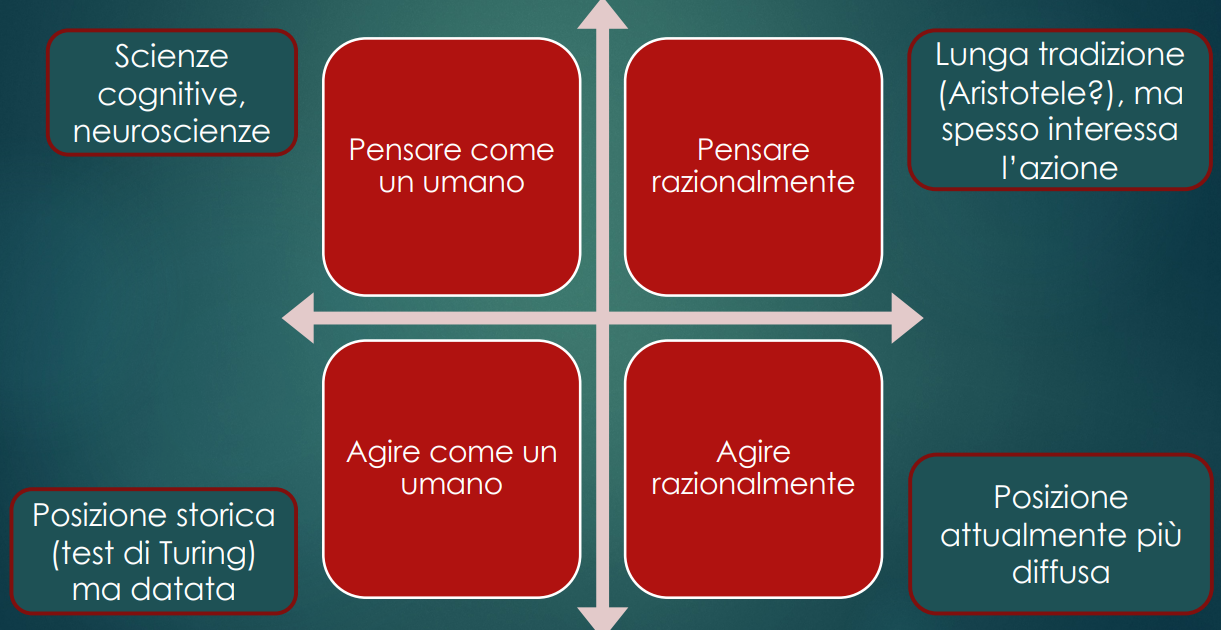
\includegraphics[width = 1\linewidth]{Images/1.PNG}
\end{center}
essi propongono uno schema che "astrae" i tipi di intelligenza, ponendoli su due dimensioni:
\begin{itemize}
    \item Sull'asse delle ordinate troviamo il contrasto tra \textbf{l'imitare l'essere umano} (cioè imitare il suo modo di agire) e il \textbf{pensare come un umano} (quindi il "risolvere problemi")
    \item Sull'asse delle ascisse troviamo il \textbf{contrasto tra il pensare e l'agire}
\end{itemize}
\subsection{Storia dell'intelligenza artificiale}
Il termine "intelligenza artificiale" fu coniato nell'agosto del 1955 da \textbf{John McCarty, Marvin Minsky, Allan Newell e Herbert Simon}, i quali proposero al Dartmouth College di Hanover (New Hampshire) di organizzare il "Dartmouth College Summer Research Project on Artificial Intelligence"; cioè uno spazio
dove accogliere persone che volessero discutere del tema dell'intelligenza artificiale. Essi descrissero l'iniziativa nel seguente modo:
\begin{center}
    "Lo studio dovrà procedere sulla base della congettura che ogni aspetto dell'apprendimento o ogni altra caratteristica dell'intelligenza può essere sia, in linea di principio, descrivibile in maniera talmente precisa che una macchina può essere costruita per simularla"
\end{center} 
In realtà, la storia dell'intelligenza artificiale risale persino ad Alan Turing (1912-1954), il quale definì il cosiddetto \textbf{Test di Turing}: l'idea di questo test è che ci sia un essere umano $C$ separato fisicamente da due interlocutori, uno anch'esso umano, chiamato $B$, e l'altro una macchina, chiamata $A$, programmata in qualche modo.
$C$ non può interloquire direttamente con $A$ e $B$, tuttavia può scambiare messaggi con essi tramite un qualche sistema di comunicazione (foglietti di carta, una chat ecc...). Quando $C$, interagendo in maniera dialogica con i due interlocutori, non riesce più di una certa percentuale di volte a capire chi dei due è la macchina allora $A$ mostra un
comportamento intelligente (cioè "agisce come un essere umano", "agisce razionalmente").
\begin{center}
    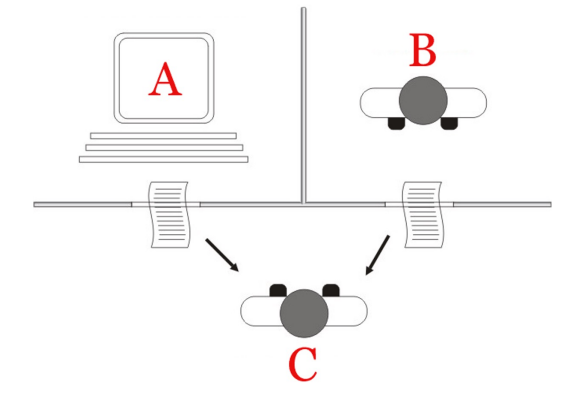
\includegraphics[width = 0.50\linewidth]{Images/2.PNG}
\end{center}
Tuttavia, nel 1966, fu prodotto un programma chiamato \textbf{ELIZA}, il quale imitava uno \textbf{psicoterapeuta}, che \textbf{superò il test di Turing nonostante fosse basato su regole di pattern matching con espressioni regolari}. Il programma portava l'utente ad avere una
\textbf{conversazione plausibile}, cioè davano all'utente l'illusione di star parlando con un \textbf{essere umano}. Per questo, il test di Turing ha solo un \textbf{interesse storico} e risulta poco interessante.
Non è quindi un caso che, nel gruppo di studio citato sopra, una delle cose di cui ci si è occupati non fosse dedicata subito all'apprendimento ma al \textbf{ragionamento}.
\subsection{Approcci simbolici}
La disciplina che si occupa delle forme corrette di ragionamento è la \textbf{logica}.
La logica è quindi lo studio sistematico delle \textbf{forme di inferenza valida}, cioè forme di elaborazione e rappresentazione della conoscenza
che garantiscono che da informazioni vere si derivino informazioni vere.
La \textbf{logica computazionale} è l'uso della logica per effettuare ragionamenti riguardo alla computazione (es. dimostrazione della correttezza di un programma).
Alcuni sforzi iniziali nel settore dell'intelligenza artificiale erano legati alla realizzazione di \textbf{dimostratori automatici di teoremi}. \newline 
Un'\textbf{inferenza} è un ragionamento che stabilisce delle relazioni tra \textbf{premesse} e delle \textbf{conclusioni}. I \textbf{modelli computazionali} di inferenza si interessano quindi di:
\begin{itemize}
    \item Quali informazioni possono trarre dato un insieme di premesse?
    \item Perché la conclusione è corretta?
\end{itemize}
L'inferenza riguarda quindi il trarre delle conclusioni quando \textbf{le premesse sono vere}.
Dire che un'inferenza è corretta, tuttavia, \textbf{non dice nulla sul valore di verità delle conclusioni}, quindi un ragionamento può essere corretto anche se \textbf{le premesse sono false}.
Le varie forme di inferenza sono:
\begin{itemize}
    \item \textbf{Deduzione}:"Se le premesse sono vere, allora le conseguenze devono essere anch'esse vere". Questa forma di ragionamento parte da delle premesse \textbf{generali} e trae delle conclusioni \textbf{particolari}
    \item \textbf{Inferenze di "senso comune"}: Esse non sono sempre "valide", ma sono \textbf{utili nella pratica}; sono modelli per spiegare \textbf{quando un inferenza è giustificata} e calcolarla di conseguenza. Esempi di questo tipo di inferenze sono:
    \begin{itemize}
        \item \textbf{Induzione}: Questa forma di ragionamento parte da delle \textbf{osservazioni particolari} e arriva a delle \textbf{conclusioni generali}.
        \item \textbf{Abduzione}: Sillogismo in cui la premessa maggiore è certa e la premessa minore è probabile, per cui anche la conclusione risulta solo probabile.
    \end{itemize}
\end{itemize}
Dove si applica quindi l'IA di tipo simbolico?
\begin{itemize}
    \item Problemi che possono essere espressi in termini di \textbf{vincoli} che devono essere soddisfatti
    \item Situazioni in cui si devono studiare delle \textbf{sequenze di azioni} per portare un certo stato dell'ambiente circostante ad un determinato obbiettivo
\end{itemize}
In passato, si svilupparono applicazioni il cui obbiettivo era \textbf{risolvere problemi specifici e delimitati}; questa applicazioni presero il nome di \textbf{sistemi esperti}.
Degli esempi notevoli sono:
\begin{itemize}
    \item \textbf{Dendral}(Anni '60): Automatizzò il processo di decisione e l'approccio alla risoluzione dei problemi dei chimici organici
    \item \textbf{Mycin}(Anni '70): Supportò  l'identificazione dei batteri che causavano infezioni gravi e la raccomandazione di antibiotici 
\end{itemize}
\begin{center}
    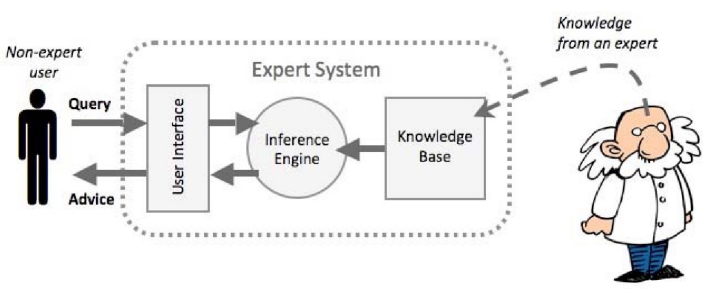
\includegraphics[width = 0.80\linewidth]{Images/3.PNG}
\end{center}
Tuttavia, presto divennero evidenti i \textbf{limiti} dei sistemi esperti:
\begin{itemize}
    \item È necessario trovare un \textbf{esperto disposto a codificare la sua conoscenza all'interno della base di conoscenza}
    \item I sistemi esperti \textbf{non scalano bene con grandi quantità di informazioni}: l'aggiornamento del sistema esperto rispetto ai \textbf{nuovi approcci alla risoluzione del problema per cui è stato costruito} è particolarmente complesso, sopratutto se il problema \textbf{non è ben delimitato}. La base di conoscenza del sistema rischierebbe quindi di \textbf{contenere troppi assiomi e regole}.
    \item Il costo di sviluppo di questi sistemi è \textbf{elevato}
\end{itemize}
\subsection{Approcci sub-simbolici}
I sistemi di IA \textbf{sub-simbolici} \textbf{non manipolano una rappresentazione simbolica} per trovare soluzioni a problemi, ma effettuano \textbf{calcoli secondo alcuni principi} che hanno dimostrato di essere in grado di portare alla risoluzione del problema.
Esempi notevoli sono:
\begin{itemize}
    \item Algoritmi genetici
    \item Reti Neurali
    \item "Intelligenza dello sciame" (Swarm Intelligence)
\end{itemize}
Tuttavia, l'argomento più importante correntemente è quello del \textbf{Machine Learning}.
Le \textbf{reti neurali artificiali} (Artificial Neural Networks (ANN)) sono una simulazione astratta del nostro sistema nervoso, il quale
contiene una collezione di \textbf{neuroni} che comunicano tra loro tramite delle connessioni dette \textbf{assoni}.
\begin{center}
    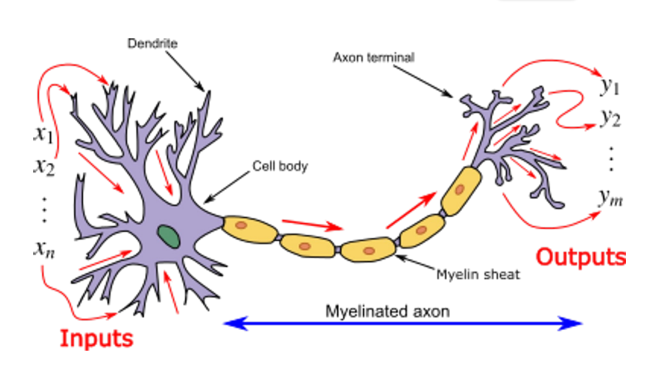
\includegraphics[width = 0.60\linewidth]{Images/4.PNG}
\end{center}
Il modello delle ANN ha delle certe somiglianze con gli assoni e i dendriti nel nostro sistema nervoso.
Il primo modello di rete neurale artificiale fu proposto nel 1943 da \textbf{McCulloch} e \textbf{Pits} nei termini di un \textbf{modello computazione dell'attività neurale}.
Questo modello fu poi seguito da altri modelli proposti da \textbf{John Von Neumann, Marvin Minsky, Frank Rosenblatt} e molti altri.
Rosenblatt definì un modello "algebrico" del neurone, chiamato \textbf{percettrone}; esso è una pietra miliare della ricerca sulle reti neurali.
Il percettrone cerca di \textbf{simulare le operazioni svolte da un singolo neurone}; l'apprendimento quindi diventa un problema di \textbf{scegliere i pesi e le soglie corrette}.
\begin{center}
    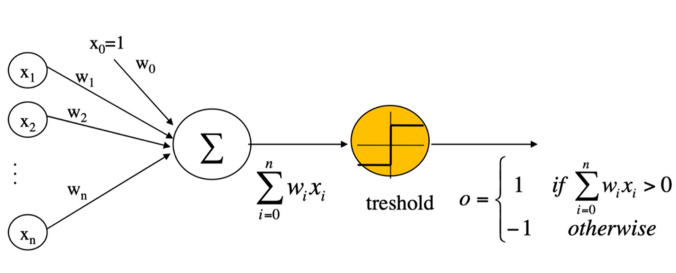
\includegraphics[width = 0.70\linewidth]{Images/5.PNG}
\end{center}
tendenzialmente, si arriva ad avere dei \textbf{percettroni multistrato}, dove ogni nodo è un singolo percettrone (introdotti per la prima volta da Minksy e S.Papert nel 1969)
\begin{center}
    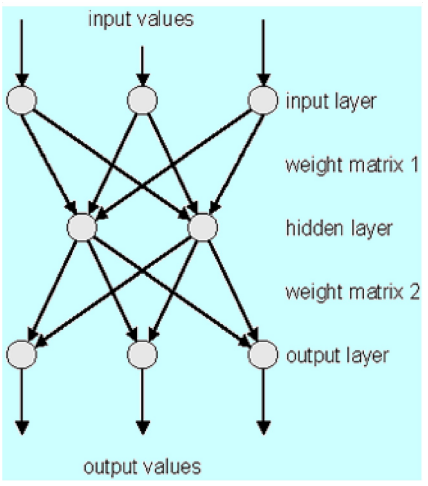
\includegraphics[width = 0.40\linewidth]{Images/6.PNG}
\end{center}
come faccio però a determinare i pesi di tutta la rete? Si utilizza il meccanismo della \textbf{back-propagation}: l'idea è che l'input è una \textbf{rappresentazione del problema} e che vi sia un \textbf{output desiderato} che la rete deve offrire;
inizialmente la rete neurale ha \textbf{dei pesi causali}, che verranno corretti \textbf{retropropagando} l'output desiderato sulla rete.
Questo è un approccio all'apprendimento che si dice "\textbf{supervisionato}".
\begin{center}
    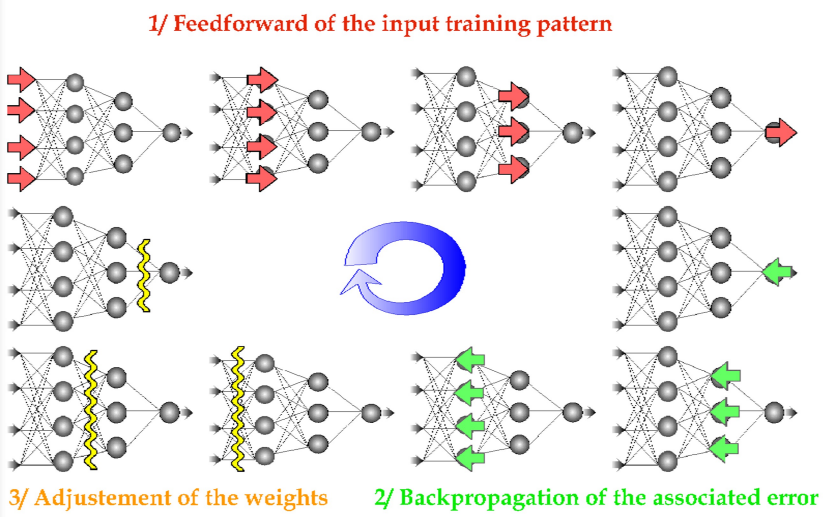
\includegraphics[width = 0.75\linewidth]{Images/7.PNG}
\end{center}
Oltre all'apprendimento supervisionato, esistono molte altre tecniche di addestramento:
\begin{center}
    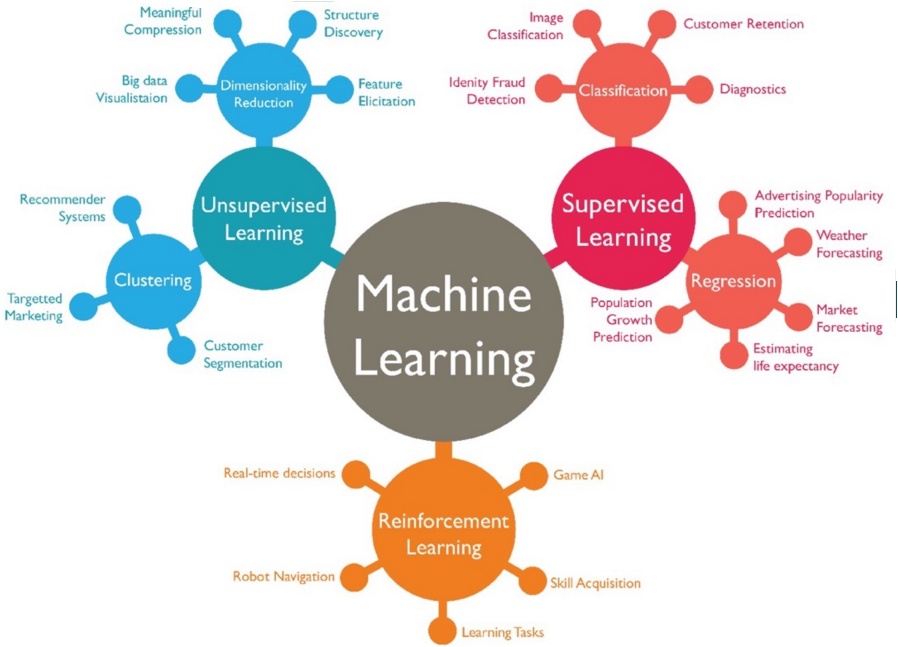
\includegraphics[width = 0.95\linewidth]{Images/8.PNG}
\end{center}
\newpage
\subsection{Agenti intelligenti, architetture e ambienti}
Un \textbf{agente} è tutto ciò che può essere vista come "percepente il suo ambiente" attraverso dei \textbf{sensori} e che può \textbf{agire su tale ambiente} attraverso degli \textbf{attuatori}.
Come agenti possono essere quindi classificati
\begin{itemize}
    \item Gli \textbf{esseri umani}, definendo come "sensori" gli occhi, le orecchie ecc... e come attuatori la bocca, le gambe, le braccia ecc...
    \item Gli \textbf{agenti robotici}, i quali hanno telecamere e sensori ad infrarossi come sensori e vari motori come attuatori
    \item Nulla vieta che \textbf{un agente possa essere anche solamente un software}
\end{itemize} 
Un agente è quindi rappresentabile nel seguente modo:
\begin{center}
    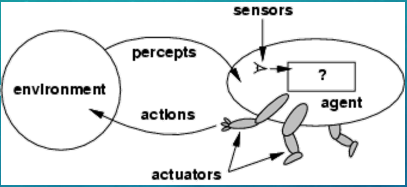
\includegraphics[width = 0.45\linewidth]{Images/9.PNG}
\end{center}
la forma più generale di agente è una \textbf{funzione} che mappa \textbf{l'insieme potenza di tutte le percezioni istantanee $\mathcal{P}^*$} ad una azione dell'insieme \textbf{di tutte le azioni eseguibili dall'agente} $\mathcal{A}$, cioè:
$$f: \mathcal{P}^* \rightarrow \mathcal{A}$$
quindi, l'agente può mappare una \textbf{sequenza arbitrariamente lunga di percezioni istantanee} (insieme potenza di $\mathcal{P}$) \textbf{ad una singola azione contenuta nell'insieme $\mathcal{A}$}.
Un agente è quindi \textbf{la sua architettura (la sua struttura profonda) più il suo programma (specifico dell'agente)}.
Gli agenti possono essere classificati, in base alla loro architettura interna, nelle seguenti classi:
\begin{itemize}
    \item Agenti con riflessi semplici
    \item Agenti con riflessi basati su un modello
    \item Agenti basati su un obbiettivo e su un modello
    \item Agenti basati su un'utilità e un modello.
\end{itemize}
\subsubsection{Agenti con riflessi semplici}
Un agente con riflessi semplici è un agente in cui vi è una comunicazione con l'ambiente (tramite i sensori e gli attuatori dell'agente).
Al suo interno, i sensori vanno a realizzare una "vista" che rappresenta \textbf{lo stato attuale dell'ambiente circostante}.
L'agente deve quindi \textbf{scegliere quale azione intraprendere} e, in questo caso, per farlo ha solamente a disposizione delle regole del tipo
\textbf{condizione-azione}.
\begin{center}
    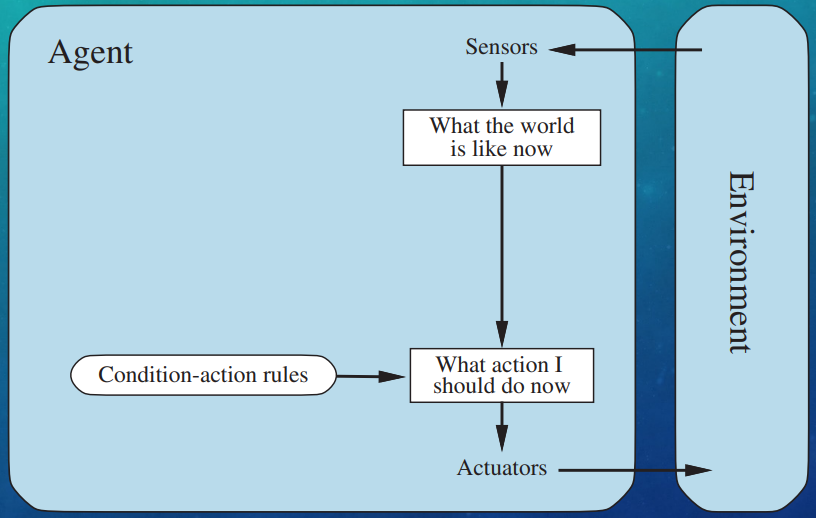
\includegraphics[width = 0.70\linewidth]{Images/10.PNG}
\end{center}
questo tipo di agente è \textbf{privo di stato}. Con architetture estremamente semplici, magari con più agenti, si riescono
quindi ad ottenere dei comportamenti, se non intelligenti, perlomeno utili.
\subsubsection{Agenti con riflessi basati su modello}
\begin{center}
    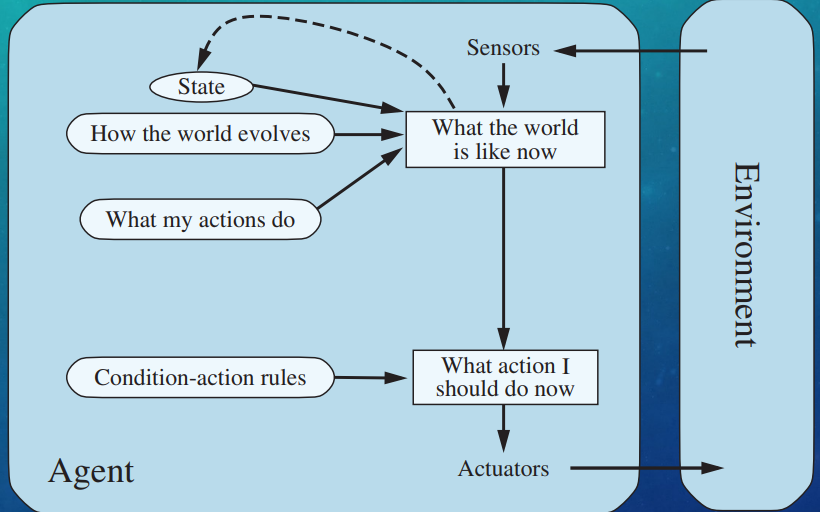
\includegraphics[width = 0.70\linewidth]{Images/11.PNG}
\end{center}
La differenza più significativa di questi agenti rispetto agli agenti con riflessi semplici è la \textbf{conoscenza del proprio stato interno}.
Questo tipo di agente può quindi \textbf{riflettere sul proprio stato} e quindi effettuare azioni basate su di esso.
Anche ignorando che l'ambiente ha una struttura, questo tipo di agente deve quindi avere un \textbf{modello matematico dell'evoluzione del mondo rispetto alle azioni fatte} che gli permetta
di decidere quale azioni intraprendere. Lo stato \textbf{non è una memoria che mantiene lo stato del mondo}, ma è solo un'informazione sullo stato dell'agente.
L'agente, inoltre, deve \textbf{poter percepire il proprio stato come parte dell'ambiente} (o come una "percezione esterna" o proprio come uno stato interno all'agente e che esso aggiorna e conosce).
Questo tipo di agente quindi può eseguire \textbf{comportamenti più adattivi rispetto all'ambiente}.
\subsubsection{Agenti basati su un obbiettivo e su un modello}
\begin{center}
    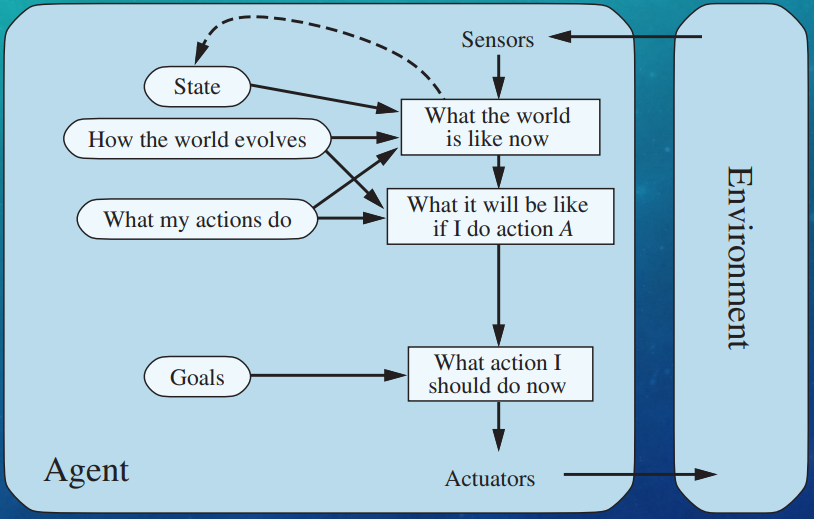
\includegraphics[width = 0.70\linewidth]{Images/12.PNG}
\end{center}
Questo tipo di agente, tramite i sensori ed eventualmente l'informazione di stato, si fa un'idea dello stato in cui si trova.
Questo agente presenta una \textbf{funzione che, partendo dallo stato dell'agente, ritorna tutte le azioni ammissibili che l'agente può intraprendere}.
Lo stato attuale viene quindi messo come \textbf{radice di un albero} e generiamo, a partire da esso, un numero di figli pari al numero di azioni ammissibili.
Possiamo costruire questo albero perché sappiamo \textbf{in quale stato si andrà a finire eseguendo una determinata azione}.
Per ogni nodo di stato che viene generato in questo modo, potremmo generare \textbf{un ulteriore livello di approfondimento dell'albero}, cioè ogni nodo stato potrebbe diventare la radice di un ulteriore sotto-albero.
In linea di principio, potrei quindi costruire l'albero di \textbf{tutti gli stati raggiungibili possibili tramite ogni combinazione possibile di azioni}.
Ovviamente, il fattore di ramificazione di questo albero è \textbf{estremamente elevato}. L'agente deve quindi esplorare questo albero per capire se esistono delle configurazioni nelle quali \textbf{l'obbiettivo sia verificato}.
Vi è quindi una \textbf{costruzione dello spazio degli stati} e una \textbf{ricerca nello spazio degli stati}. \newline
Per capire quali azioni intraprende, l'agente deve quindi risolvere un \textbf{problema di ricerca}, il quale consiste in:
\begin{itemize}
    \item Uno \textbf{spazio degli stati}
    \item Una \textbf{funzione di successione}, che dato un certo stato e l'azione che si vuole intraprendere (la quale potrebbe avere un certo \textbf{costo}), in quale stato si vada a finire. Questa funzione mi dice anche \textbf{quali sono le azioni ammissibili in un determinato stato}
    \item Uno \textbf{stato iniziale}
    \item Una \textbf{funzione "goal test"} che ci dica \textbf{se l'obbiettivo è stato raggiunto o meno}
\end{itemize}
Una \textbf{soluzione} ad un problema di ricerca è una \textbf{sequenza di azioni} (un piano) che trasformano lo stato iniziale nello stato obbiettivo.
Uno \textbf{spazio di ricerca} astrae l'ambiente per selezionare solo le informazioni utili per risolvere il problema.
\begin{center}
    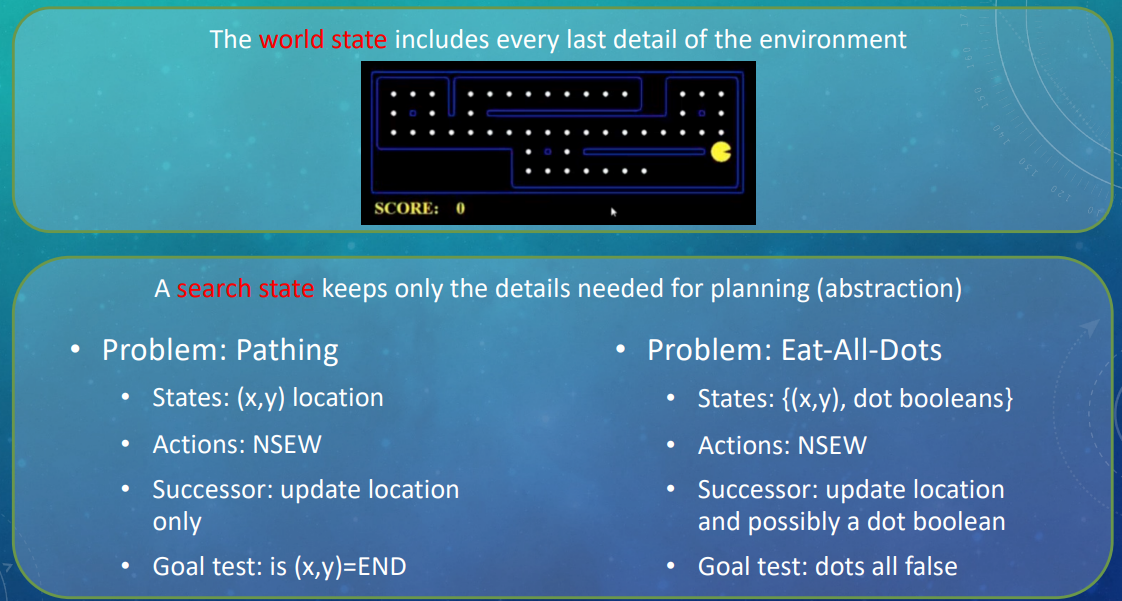
\includegraphics[width = 1\linewidth]{Images/13.PNG}
\end{center}
lo spazio degli stati, per problemi di ragionevole complessità, \textbf{tendono ad esplodere}, quindi non si possono applicare generalmente algoritmi \textbf{forza bruta} per trovare una configurazione che risolva il problema.
La costruzione dello spazio di ricerca avviene tramite \textbf{un albero di ricerca}, dove:
\begin{itemize}
    \item Lo stato iniziale è il nodo radice
    \item I figli corrispondono agli stati successivi data un'azione
    \item I nodi mostrano gli stati, ma \textbf{corrispondono ai piani per raggiungere quelli stati}
    \item Per la maggior parte dei problemi, non arriviamo mai a costruire l'intero albero (troppo grande)
\end{itemize}
\begin{center}
    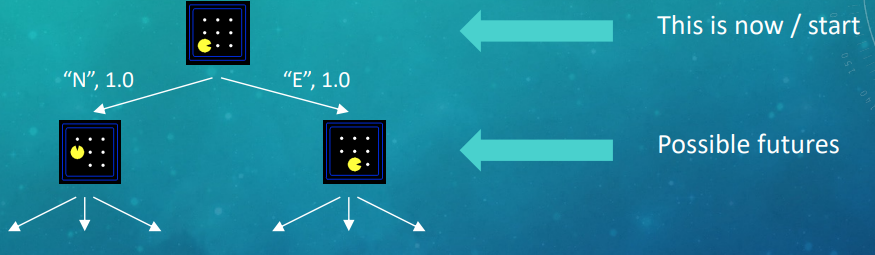
\includegraphics[width = 1\linewidth]{Images/14.PNG}
\end{center}
Invece di usare un albero per rappresentare il problema di ricerca, potremmo invece usare un \textbf{grafo dello spazio degli stati}: esso da una rappresentazione matematica del problema di ricerca nel seguente modo:
\begin{itemize}
    \item I nodi sono \textbf{le possibili configurazioni del mondo}
    \item Gli archi rappresentano \textbf{i risultati delle azioni}
    \item La funzione \textbf{"goal test"} viene rappresentata da un \textbf{insieme di nodi}
\end{itemize}
\begin{center}
    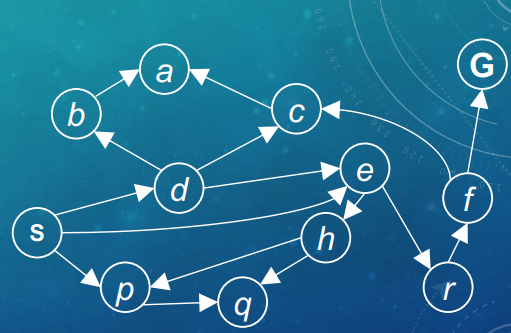
\includegraphics[width = 0.50\linewidth]{Images/15.PNG}
\end{center}
In un grafo dello spazio degli stati, \textbf{ogni stato occorre solamente una volta!} Tuttavia, raramente possiamo costruire l'intero grafo in memoria, poiché \textbf{esso cresce troppo velocemente}; tuttavia è un'idea utile.
Qual'è quindi la differenza sostanziale tra un grafo dello spazio degli stati e un albero di ricerca? Ogni \textbf{nodo} in un albero di ricerca è l'equivalente di un \textbf{intero cammino sul grafo dello spazio degli stati}.
Entrambi devono essere costruiti \textbf{"on demand"} (cioè li espandiamo solamente quando occorre) e devono esser espansi il meno possibile.
\subsubsection{Agenti basati su un'utilità e un modello}
\begin{center}
    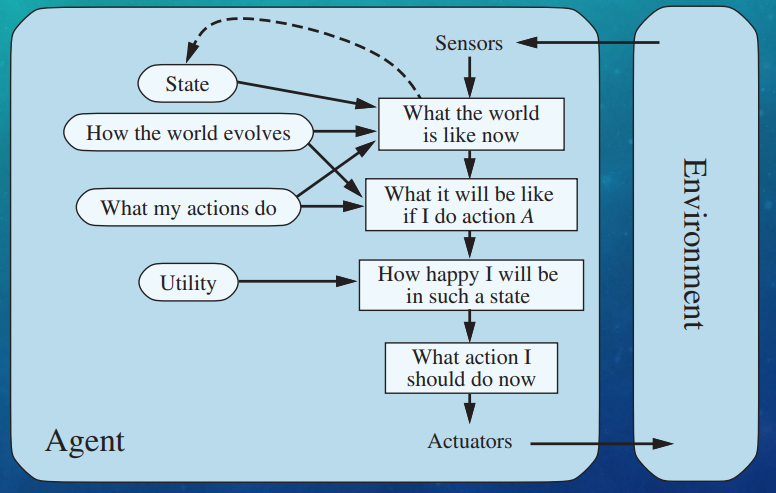
\includegraphics[width = 0.80\linewidth]{Images/16.PNG}
\end{center}
La differenza di questo tipo di agente con il precedente è la \textbf{scomparsa della funzione "goal test"} e l'introduzione di una \textbf{funzione "Utility"}, la quale è una vera e propria funzione
che attribuisce ad un certo stato del mondo un idea di \textbf{quanto quello stato sia desiderabile dall'agente}. Perché? Ci sono diversi motivi:
\begin{itemize}
    \item Potrei non essere in grado di definire formalmente una funzione che descriva l'obbiettivo
    \item Dato lo stato dell'ambiente, posso definire una funzione che valuti i vari elementi di esso e mi permetta di effettuare valutazione sulla prossima aziona da eseguire (es. scacchi)
    \item Avere una funzione d'utilità mi permette di considerare obbiettivi contrastanti fra loro; quindi poter definire una funzione che valuti tutti i fattori in gioco e che possa portare alla \textbf{discriminazione di certi stati} (es. problema di logistica)
\end{itemize}
\subsubsection{Caratteristiche dell'ambiente}
Russel e Norvig definiscono una serie di caratteristiche per l'ambiente:
\begin{itemize}
    \item \textbf{Ambienti accessibili vs Inaccessibili}: Un \textbf{ambiente accessibile} è un ambiente dove l'agente può ottenere un informazione \textbf{completa, accurata e aggiornata} riguardo lo stato dell'ambiente.
    Molti ambiente moderatamente complessi (includendo, per esempio, il mondo fisico e internet) sono \textbf{inaccessibili}. Più un ambiente è accessibile, più è semplice costruire un agente che possa operare in esso.
    I problemi di accessibilità del mondo si presentano ogni qualvolta che ci accingiamo a risolvere problemi nel \textbf{mondo fisico}
    \item \textbf{Ambienti deterministici vs non-deterministici}: Un \textbf{ambiente deterministico} è un ambiente in cui ogni azione ha un singolo effetto garantito: non c'è \textbf{incertezza} riguardo allo stato in cui l'ambiente si troverà in seguito al compiersi di un azione. Il mondo fisico dovrebbe essere sempre considerato come sostanzialmente \textbf{non-deterministico}, salvo certi casi in cui si può pensare come deterministico.
    Gli ambienti non-deterministici presentano problemi maggiore per il progettista dell'agente.
    \item \textbf{Ambienti episodici vs sequenziali}: In un ambiente \textbf{episodico}, l'esperienza dell'agente può essere divisa in \textbf{passi atomici} dove l'agente percepisce uno stimolo ed effettua una singola azione. La scelta dell'azione da intraprendere \textbf{dipende solamente dall'episodio stesso}.
    Gli ambienti episodici sono più semplici dal punto di vista del progettista dell'agente, poiché l'agente può decidere quale azione intraprendere basandosi solo sull'episodio corrente, \textbf{non deve quindi ragionare riguardo all'interazione tra questo episodio e quelli futuri}.
    \item \textbf{Ambienti statici vs dinamici}: Per \textbf{ambiente statico} si intende un ambiente che \textbf{non cambia nel mentre che l'agente sta decidendo l'azione da compiere}; un cambiamento in un ambiente statico avviene quindi \textbf{solamente a causa di un'azione da parte dell'agente}.
    Per \textbf{ambiente dinamico} si intende un ambiente che \textbf{cambia mentre l'agente sta decidendo quale azione intraprendere} e che quindi ha al suo interno altri processi, oltre all'agente, che ne modificano lo stato e le cui azioni possono interferire con le azioni dell'agente (come nella teoria dei sistemi concorrenti); le trasformazioni di un ambiente dinamico quindi avvengono \textbf{al di fuori del controllo dell'agente}.
    Il mondo fisico è un ambiente altamente dinamico.
    \item \textbf{Ambienti discreti vs continui}: Un \textbf{ambiente discreto} è un ambiente che presenta un numero \textbf{fissato e finito} di azioni e di percezioni in esso. Gli \textbf{ambienti continui} hanno un certo livello di \textbf{discrepanza} con i sistemi computerizzati.
    Gli ambienti discreti potrebbero essere gestiti, in linea di principio, da una specie di \textbf{tabella di ricerca} (lookup table).
    Per semplificare la gestione di un ambiente continuo, si può \textbf{sovrapporre ad esso una sua discretizzazione} in modo da rendere più semplice la progettazione e l'implementazione degli agenti che devono operare al suo interno.
\end{itemize} 
\begin{center}
    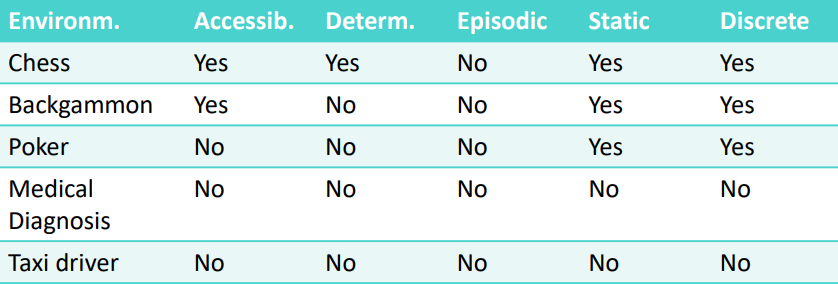
\includegraphics[width = 0.80\linewidth]{Images/17.PNG}
\end{center}
\section{Approcci simbolici - Planning}
Come abbiamo visto, definire in maniera precisa cos'è l'intelligenza è un compito piuttosto complicato.
La ricerca di una definizione univoca ha portato a definizioni di intelligenza \textbf{più focalizzate sulle singole funzioni} e ha portato alla seguente distinzione in termini di performance:
\begin{center}
    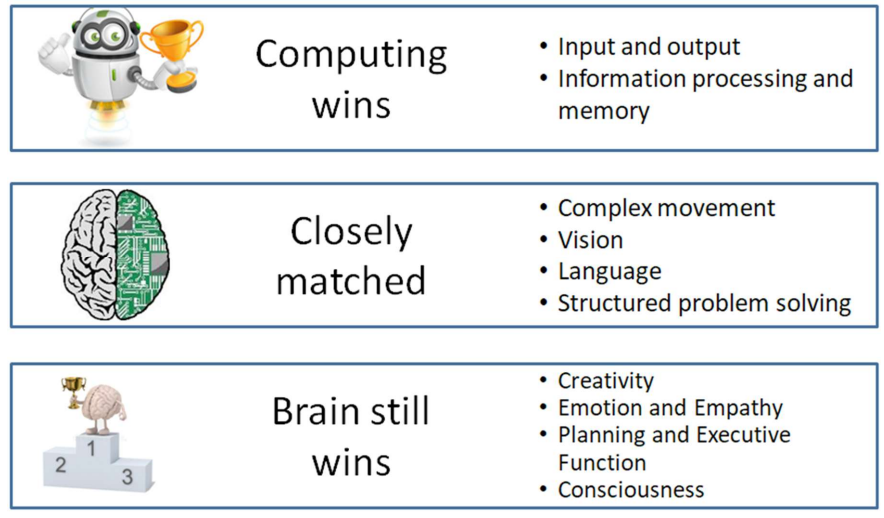
\includegraphics[width = 0.80\linewidth]{Images/18.PNG}
\end{center}
abbiamo quindi dato una definizione di intelligenza basandoci su dei \textbf{compiti da svolgere}, i quali possono essere a volte dei \textbf{problemi}.
Ma quindi, cos'è effettivamente un problema? Possiamo dare la seguente definizione:
\begin{center}
    Vogliamo \textbf{realizzare una condizione desiderata}, che all'inizio non è soddisfatta. Per farlo, dobbiamo \textbf{scegliere} quali azioni intraprendere da un insieme di \textbf{possibili scelte (complesse)}.
\end{center}
Uno degli interessi di studio nel campo dell'intelligenza artificiale è anche quello di \textbf{comprendere come gli essere umani risolvono i problemi}.
Possiamo quindi partire dalla nozione di \textbf{risolutore di problemi generici}, di cui una versione possibile è la seguente:
\begin{center}
    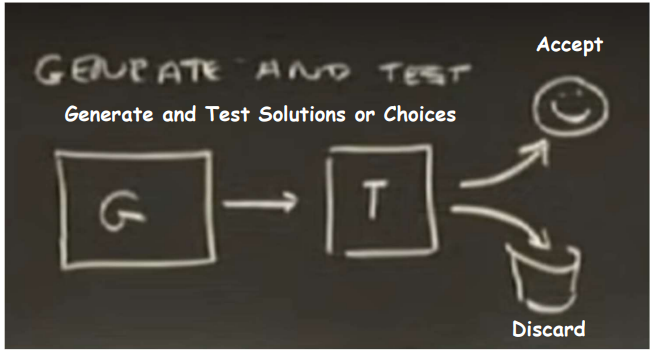
\includegraphics[width = 0.60\linewidth]{Images/19.PNG}
\end{center}
quando questa soluzione può essere inefficiente oppure quando essa può fallire?
\begin{itemize}
    \item Una fonte di inefficienza può essere la \textbf{necessità di effettuare un test su tutte le condizioni generate}
    \item Il costo di una soluzione \textbf{potrebbe essere elevato sia dal punto di vista economico che umano}
    \item Generare le soluzioni ha un costo
    \item Questo sistema può fallire non solo \textbf{quando le possibili scelte sono tante} ma anche quando il generatore \textbf{non riesce a generare tutte le possibili soluzioni oppure esse sono infinite} 
\end{itemize}
nonostante le problematiche sopra, il fatto di \textbf{poter enumerare e valutare tutte le possibili soluzioni al problema} è già un modo di risolverlo quando il suo spazio delle soluzioni (e quindi delle scelte) è limitato.
Ci sono varie condizioni dove si possono applicare, in maniera efficiente, questo tipo di risolutori; alcuni esempi sono:
\begin{itemize}
    \item \textbf{Risolvere puzzle}: In questo caso, la condizione desiderata è \textbf{raggiungere la configurazione base del puzzle} (es. il cubo di rubik con tutte le facce di un certo colore) in una certa maniera (più velocemente? con meno azioni possibili? ecc...)
    La condizione iniziale \textbf{è una configurazione randomica del puzzle}. In questo caso, dobbiamo produrre la sequenza di tutte le azioni necessarie per arrivare alla condizione desiderata rispettando i limiti di tempo/mosse dati.
    Le \textbf{scelte} in questo caso sono \textbf{le sequenza di cambiamenti (complessi) nella configurazione del puzzle}, mentre le \textbf{azioni} sono invece ciò che ci permette di muoverci da una configurazione del puzzle all'altra per creare, concatenandole in sequenza, delle \textbf{scelte} che possano essere valutate rispetto al nostro obbiettivo.
    Ovviamente, per esempio, raggiungere l'obbiettivo con il minor numero di mosse possibili \textbf{non è detto che sia la maniera più veloce} e viceversa.
    \newpage
    \item \textbf{Pacman}:
    \begin{itemize}
        \item \textbf{Condizione desiderata}: mangiare la pillola più vicina? Mangiare tutte le pillole il più velocemente possibile?
        \item \textbf{Inizialmente}: Pacman si trova da qualche parte all'interno del labirinto
        \item \textbf{Scelte}: Strada 1, Strada 2, ..., Strada $N + 1$
        \item \textbf{Azioni}: su, giù, sinistra, destra
    \end{itemize}
    \item ...
\end{itemize}
ciò che hanno in comunque questi esempi è che entrambi presentano delle \textbf{condizioni}, cioè degli \textbf{stati}.
Partendo da una configurazione iniziale e compiendo un'azione, ci troviamo in una configurazione successiva, in cui possiamo compiere
un'altra azione ed arrivare ad un'altra configurazione. L'iterazione di questo processo ci permette di creare \textbf{sequenze di cambiamenti} (le scelte) e quindi di \textbf{generare ogni possibile configurazione del problema}.
Abbiamo quindi ottenuto il generatore $G$ del risolutore sopra.
La possibilità di testare se la configurazione soddisfa l'obbiettivo dipende da come definiamo la configurazione stessa.
Ciò che resta da fare è quindi trovare dei buoni modi per implementare i generatori di soluzioni $G$ e per testare le soluzioni che generano velocemente.
\subsection{Problemi di ricerca}
Come abbiamo visto, le soluzioni possono essere costruite come \textbf{sequenze di stati (o configurazioni e azioni che le cambiano)}.
I tipi di problemi che abbiamo visto sopra si dicono \textbf{problemi di ricerca}, nei quali abbiamo:
\begin{itemize}
    \item Uno \textbf{spazio degli stati} (insieme degli stati) $\mathcal{S}$
    \item Uno \textbf{stato iniziale} $s_0$
    \item Un \textbf{insieme delle azioni possibili in ogni stato} $\mathcal{A}(\mathcal{s})$
    \item Una \textbf{funzione di successione/transizione} $s' = next$
    \item Un \textbf{"goal test"} $G(s)$ che dice se abbiamo raggiunto l'obbiettivo
    \item Un \textbf{costo per ogni azione} $c(s, a, s')$ (opzionale)
    \item 
\end{itemize}
Una \textbf{soluzione ad un problema di ricerca} è una sequenza di azioni (un piano) che trasforma lo stato iniziale in uno \textbf{stato obbiettivo}, cioè in uno stato che soddisfi il \textbf{goal test}.
Una \textbf{soluzione ottimale} ha il \textbf{costo minore tra tutte le possibili soluzioni}.
Lo stato di un problema \textbf{può essere rappresentato in molti modi diversi} (es. pixel, spazio degli stati ecc...).
Per evitare di complicare troppo il problema di ricerca definendo uno spazio degli stati inefficiente, possiamo seguire le \textbf{condizioni di Markov sugli stati, sui successori e sul goal test}:
\begin{itemize}
    \item L'efficienza richiede un \textbf{insieme degli stati il più piccolo possibile}; tuttavia esso deve soddisfare le seguente condizioni:
    \begin{enumerate}
        \item Data una funzione di transizione, uno stato \textbf{contiene tutte le informazioni necessarie per arrivare all'obbiettivo tramite la scelta di azioni da intraprendere}
        \item Dato lo stato $s(t)$, il risultato $s(t+1) = next(s(t), a(t))$ della prossima azione $a(t)$ non dipende dagli stati precedenti $s(t')$ o dalle azioni precedenti
        \item Il goal test può essere applicato direttamente agli stati senza che sia richiesta dell'altra informazione aggiuntiva.
    \end{enumerate}
\end{itemize}
\begin{center}
    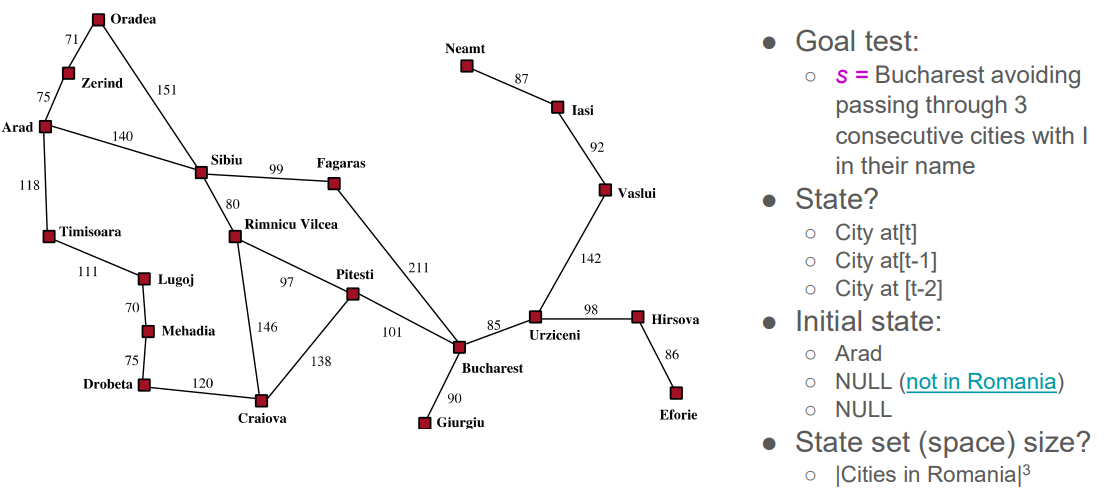
\includegraphics[width = 1\linewidth]{Images/20.PNG}
\end{center}
La condizione in cui risolvere un problema di ricerca risulta più semplice è quando \textbf{il numero degli stati e delle azioni è finito} e \textbf{per ogni azione, c'è un solo possibile stato di destinazione che si raggiunge}.
Per risolvere un problema con la ricerca, ciò che possiamo fare è quindi generare \textbf{tutte le configurazioni a cui le azioni possibili in un certo stato $s$ portano} e poi scegliere quali
di esse espandere ulteriormente. La scelta di \textbf{quale configurazione espandere determina il comportamento dell'agente durante la risoluzione del problema} (esso, per esempio, potrebbe anche entrare in un loop infinito).
Facciamo un esempio: dato il seguente problema:
\begin{center}
    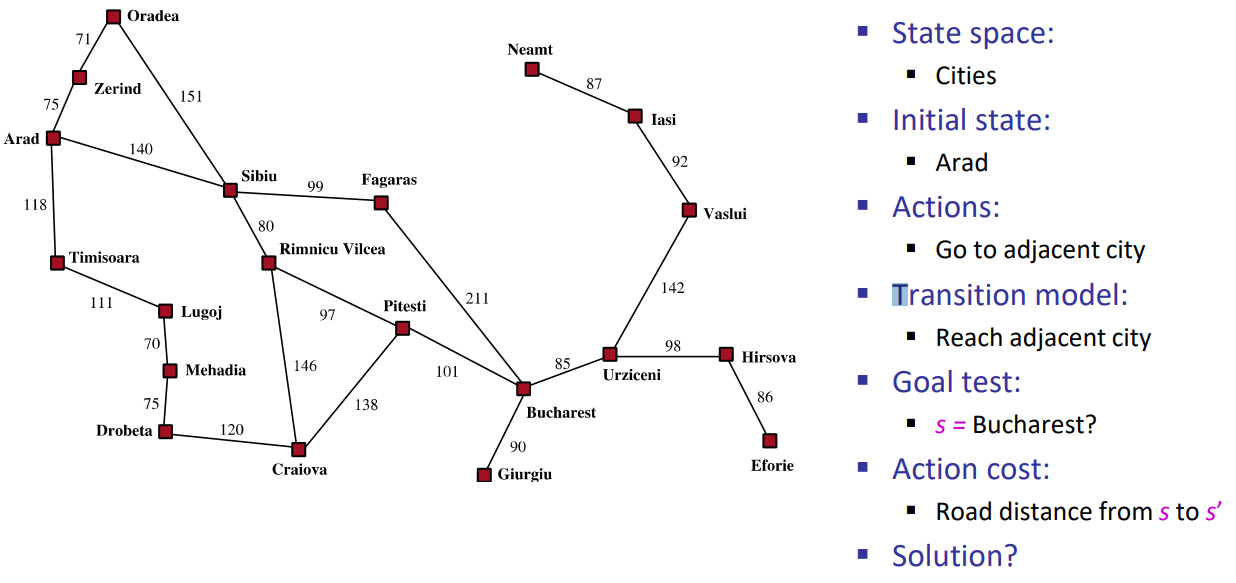
\includegraphics[width = 1\linewidth]{Images/21.PNG}
\end{center}
allora un algoritmo che l'agente può seguire per risolvere il problema è il seguente:
\begin{center}
    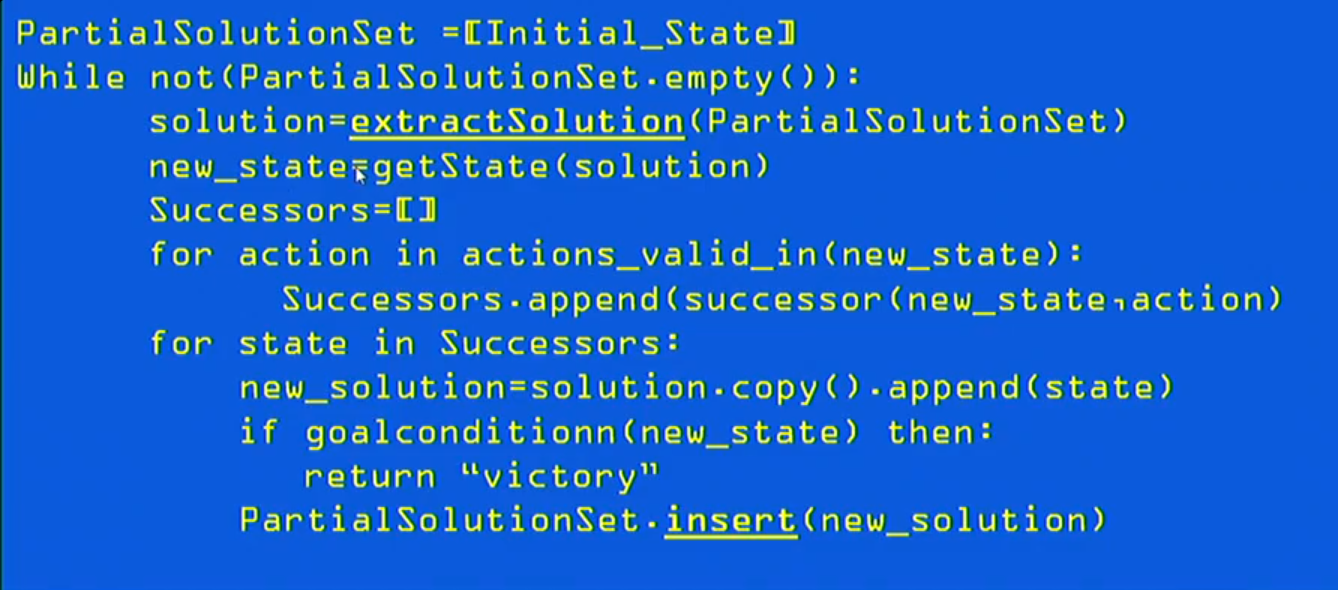
\includegraphics[width = 1\linewidth]{Images/22.PNG}
\end{center}
il modo in cui estraiamo una soluzione o ne aggiungiamo una nuova influenza l'efficienza dell'algoritmo.
Cambiando la struttura dati sottostante, viene inoltre cambiato \textbf{il comportamento dell'agente e le sue performance}.
Consideriamo ora un \textbf{agente basato su riflessi}; quando l'agente riceve un input $x$, allora esso effettua l'azione associata
a quell'input; quindi, se $f$ è la funzione che determina quale azione intraprendere, si può vedere l'agente in questo modo:
$$x \Rightarrow f \Rightarrow \textrm{singola azione } y \in \{-1, +1\}$$
Tuttavia, è piuttosto complesso costruire agenti di questo tipo per risolvere problemi di ricerca. Si preferisce quindi avere
agenti \textbf{basati sullo stato} che effettuano una simulazione interna e che siano in grado di \textbf{tenere traccia delle conseguenze delle proprie azioni} per arrivare alla soluzione:
$$x \Rightarrow f \Rightarrow \textrm{sequenza di azioni } (a_1, a_2, \dots)$$
tuttavia, abbiamo bisogno di questo tipo di agenti? Non potremmo risolvere questi problemi "senza pensare"?
\begin{itemize}
    \item Potremmo, in linea di principio, usare un agente basato su riflessi per risolvere un problema di ricerca? Potremmo creare una tabella di ricerca per determinare ogni nuovo stato a partire a seconda dell'azione intrapresa, ma solo sotto certe condizioni:
    \begin{itemize}
        \item L'informazione disponibile deve essere sempre sufficiente per poter effettuare una scelta
        \item Se non ci sono problemi di informazione, allora si potrebbe utilizzare una mappa degli stati per risolvere il problema di ricerca
    \end{itemize}
    \item Il problema principale a questo tipo di approccio è \textbf{il numero delle possibili configurazioni del problema}, visto che per ogni possibile configurazione è necessario avere una soluzione.
    \item Poiché le configurazione possono essere moltissime, allora la mappa rischia di essere enorme
\end{itemize}
Dobbiamo infine ricordare che quando si risolve un problema di ricerca, utilizziamo un \textbf{modello} che astrae le informazioni necessarie a risolverlo.
Per questo motivo, \textbf{i modelli, rispetto al mondo reale, risultano quasi sempre errati}, poiché tengono conto solamente delle informazioni rilevanti per risolvere il problema.
\subsection{Search Trees e algoritmi di ricerca}
Un modo molto semplice per codificare le soluzioni parziali ed effettuare delle scelte sono gli \textbf{alberi di ricerca} (search trees).
In questo tipo di struttura dati è:
\begin{itemize}
    \item Ogni nodo è uno \textbf{stato}
    \item La radice è lo \textbf{iniziale}
    \item I figli di ogni nodo corrispondono ai suoi \textbf{successori}
    \item Una \textbf{soluzione} è un \textbf{cammino} che dalla radice porta ad una foglia che soddisfa il "Goal Test"
\end{itemize}
\begin{center}
    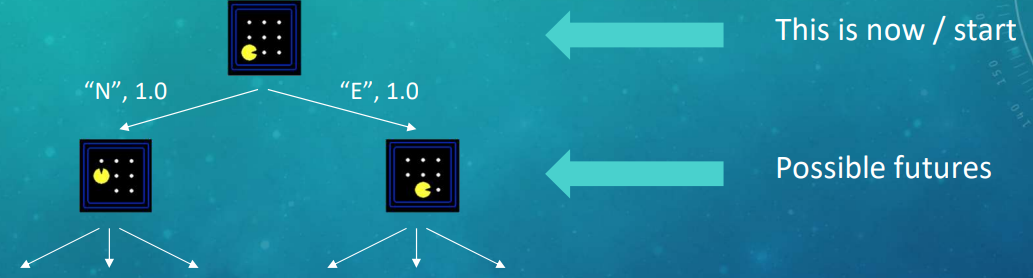
\includegraphics[width = 1\linewidth]{Images/23.PNG}
\end{center}
Un problema di questo approccio è che, a causa dell'elevato numero di stati, \textbf{non è quasi mai possibile espandere completamente l'albero di ricerca}.
Si rende quindi necessario lo sviluppo di approcci per ridurre i tempi computazionali.
\begin{center}
    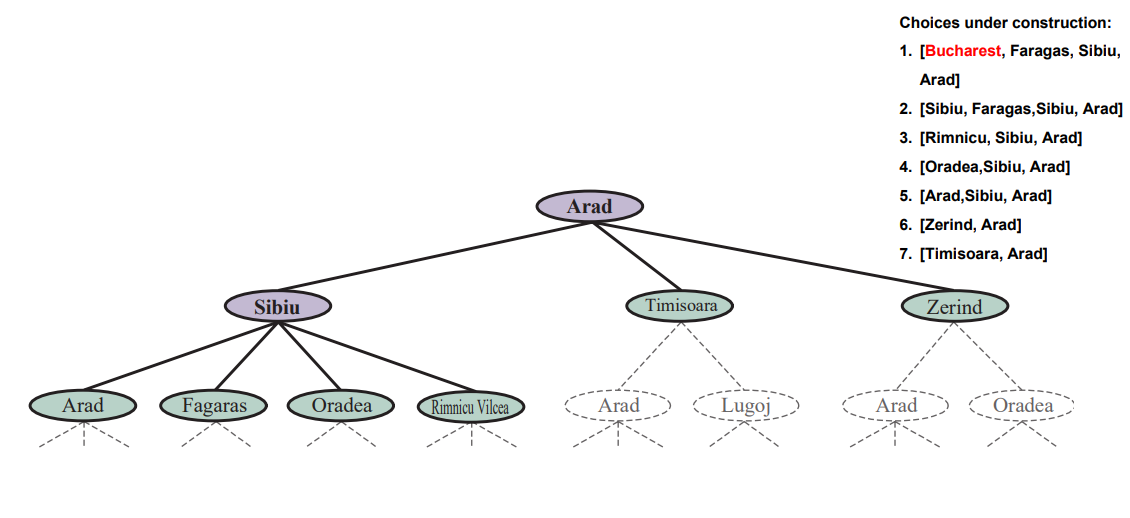
\includegraphics[width = 1\linewidth]{Images/24.PNG}
\end{center}
la differenza, quindi, tra i vari algoritmi di ricerca è il \textbf{modo in cui si sceglie di costruire ed esplorare l'albero}.
Un algoritmo generico per la \textbf{ricerca all'interno dell'albero è il seguente}:
\begin{center}
    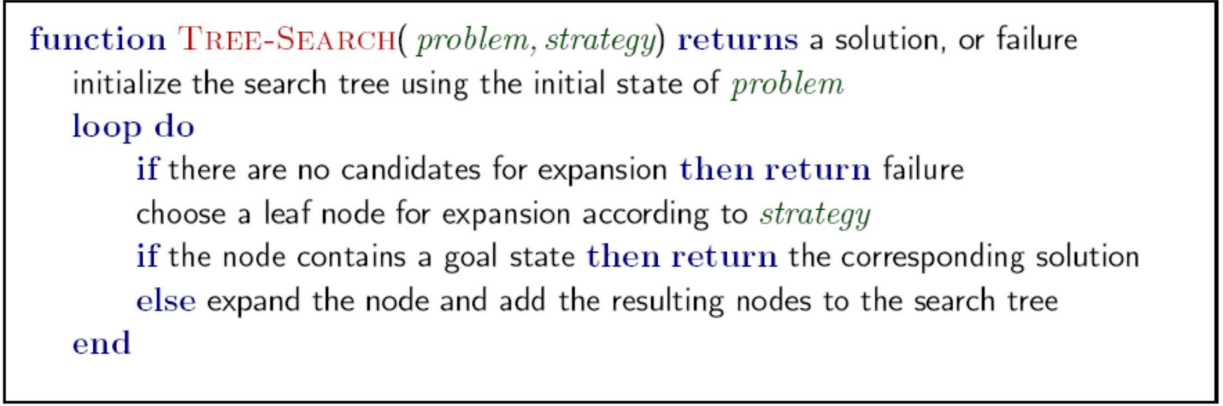
\includegraphics[width = 1\linewidth]{Images/25.PNG}
\end{center}
questa è un'implementazione basata sull'albero; la questione quindi diventa:
\begin{itemize}
    \item Quale nodo foglia espandere?
    \item Dobbiamo fare un controllo per stati ripetuti? (loop infiniti)
\end{itemize}
le proprietà di un algoritmo di ricerca generico sono le seguenti:
\begin{itemize}
    \item \textbf{Caratteristiche della ricerca}:
    \begin{itemize}
        \item \textbf{Completezza}: Garantisce di trovare una soluzione se esiste?
        \item \textbf{Ottimalità}: Garantisce di trovare il cammino di costo minimo?
    \end{itemize}
    \item Sia $b$ il \textbf{branching factor}, cioè il numero di azioni possibili per stato
    \item Sia $m$ (o $D$) la \textbf{massima profondità} a cui si può esplorare
    \item Le soluzioni possono essere a varie profondità
    \item Numero di nodi nell'intero albero? $$1 + b + b^2 + \dots + b^m = \mathcal{O}(b^m)$$
\end{itemize}
\begin{center}
    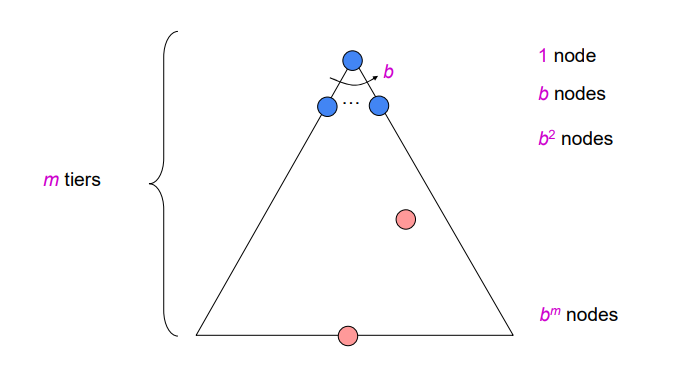
\includegraphics[width = 0.80\linewidth]{Images/29.PNG}
\end{center}
\subsubsection{Backtracking search}
Un primo algoritmo semplice che ci permette di trovare una soluzione nell'albero di ricerca
è il \textbf{Backtracking search}:
\begin{center}
    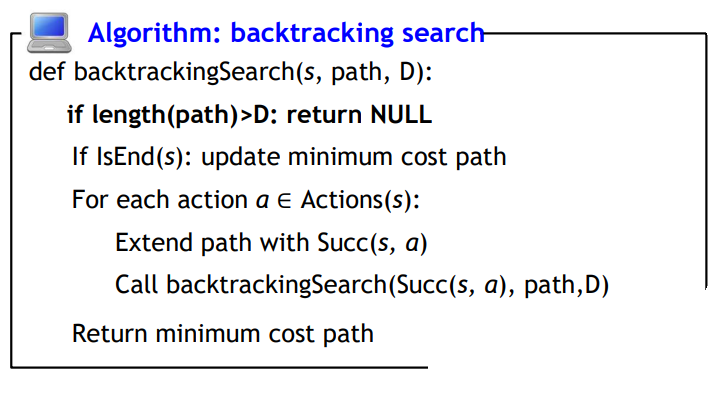
\includegraphics[width = 0.70\linewidth]{Images/26.PNG}
\end{center}
questo algoritmo espande sempre il primo nodo che non è stato espanso, fino ad arrivare ad una certa profondità.
Il limite alla profondità dell'albero permette di evitare che ci si possa fermare a causa di loop infiniti.
In questo modo, l'algoritmo \textbf{ricostruisce l'intero albero dei percorsi di lunghezza massima}, permettendo di poter effettuare
diverse domande sul nostro spazio degli stati. (es. percorso di lunghezza minima, percorso di costo minimo ecc...).
Lo svantaggio di questo algoritmo è che \textbf{deve espandere l'intero albero per trovare una soluzione} e non è detto che l'ultima soluzione trovata dall'algoritmo
\textbf{sia migliore di una soluzione trovata in precedenza}; tuttavia, questo tipo di algoritmo è estremamente flessibile, quindi si possono avere
delle condizioni arbitrarie che \textbf{impediscono all'algoritmo di continuare ad espandere l'albero in una certa direzione}.
Se abbiamo $b$ azioni possibili per stato, e un massima profondità $D$ di ricerca, allora i costi dell'algoritmo sono i seguenti:
\begin{itemize}
    \item \textbf{Memoria}: $\mathcal{O}(bD)$ (piccolo)
    \item \textbf{Tempo}: $\mathcal{O}(b^D)$ (enorme)
\end{itemize}
\subsubsection{Depth First Search}
\begin{center}
    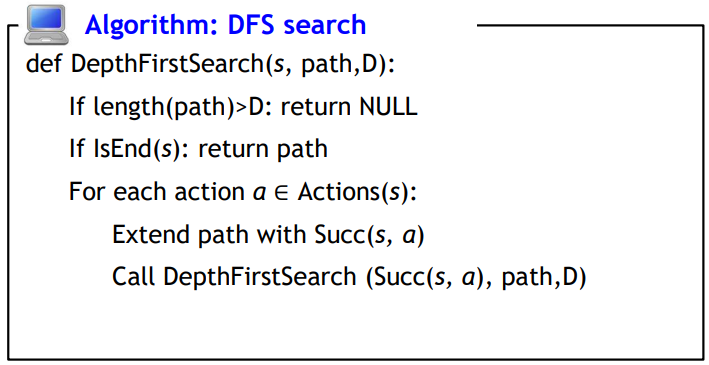
\includegraphics[width = 0.70\linewidth]{Images/27.PNG}
\end{center}
A volte, non abbiamo condizioni complesse sul percorso ma, semplicemente, il valore di una foglia (quindi lo stato attuale) ci basta per capire
se la condizione di interesse è soddisfatta. Allora, in questo caso, possiamo usare un algoritmo di ricerca in profondità (DFS).
una volta che l'algoritmo trova una soluzione, \textbf{esso termina}.
L'algoritmo, durante la sua esecuzione, \textbf{tiene in memoria solamente le informazioni relative alla soluzione}.
\begin{center}
    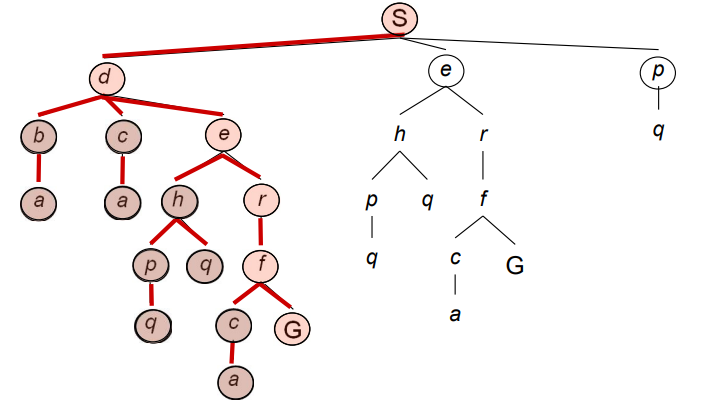
\includegraphics[width = 0.70\linewidth]{Images/28.PNG}
\end{center}
le uniche cose che bisogna memorizzare quando si effettua una DFS su un albero di ricerca sono quindi \textbf{quali nodi sono attivi nella soluzione attuale} e quali figli
di un certo nodo sono \textbf{ancora da esplorare}.
Le proprietà dell'algoritmo sono le seguenti:
\begin{itemize}
    \item Quali sono i nodi che la DFS espande?
    \begin{itemize}
        \item Espande alcuni nodi dell'albero fino ad una profondità $m$
        \item Potrebbe processare l'intero albero
    \end{itemize}
    \item \textbf{Completezza}: Poiché $m$ può essere infinito, prevenire dei cicli \textbf{potrebbe aiutare a trovare una soluzione}
    \item \textbf{Ottimalità}: L'algoritmo non è ottimale, dato che trova la \textbf{soluzione più a sinistra}, senza curarsi della profondità o del costo 
\end{itemize}
In termini di complessità, se si hanno $b$ decisioni per stato e la massima profondità permessa è $m$ si ha che:
\begin{itemize}
    \item \textbf{Spazio}: $\mathcal{O}(bm)$
    \item \textbf{Tempo}: $\mathcal{O}(b^m)$ nel caso peggiore, ma potrebbe ridursi molto se le soluzioni sono semplici da trovare
\end{itemize}
\begin{center}
    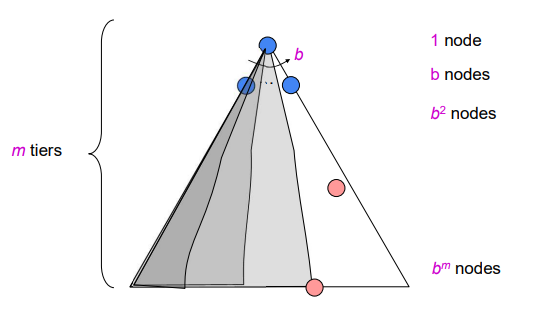
\includegraphics[width = 0.70\linewidth]{Images/30.PNG}
\end{center}
\subsubsection{Breadth First Search}
Una ricerca in ampiezza (BFS) andrà ad espandere \textbf{tutti i nodi dell'albero che si trovano allo stesso livello}. Così facendo, l'algoritmo
va a creare una \textbf{frontiera di nodi che devono essere ancora espansi}. Una volta terminati i nodi da espandere in un certo livello, l'algoritmo
passa ad espandere i nodi del livello successivo.
\begin{center}
    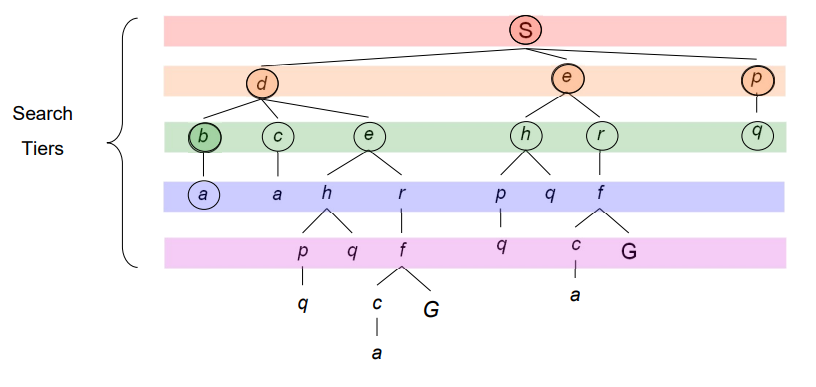
\includegraphics[width = 0.70\linewidth]{Images/31.PNG}
\end{center}
procedendo in questo modo, l'algoritmo \textbf{riesce a trovare la soluzione di costo minimo} (o quella che richiede meno passi).
Le proprietà della BFS sono le seguenti:
\begin{itemize}
    \item Quali nodi espande una BFS?
    \begin{itemize}
        \item Processa tutti i nodi sopra la soluzione meno in profondità. Sia questa profondità $s$
    \end{itemize}
    \item \textbf{Completezza}: Se $s$ è finito, allora di sicuro una soluzione esiste. L'algoritmo è completo
    \item \textbf{Ottimalità}: è ottimo solo se i costi dei cammini sono tutti \textbf{uguali}
\end{itemize}
In termini di complessità, abbiamo che:
\begin{itemize}
    \item \textbf{Spazio}: $\mathcal{O}(b^s)$
    \item \textbf{Tempo}: $\mathcal{O}(b^s)$
\end{itemize}
\begin{center}
    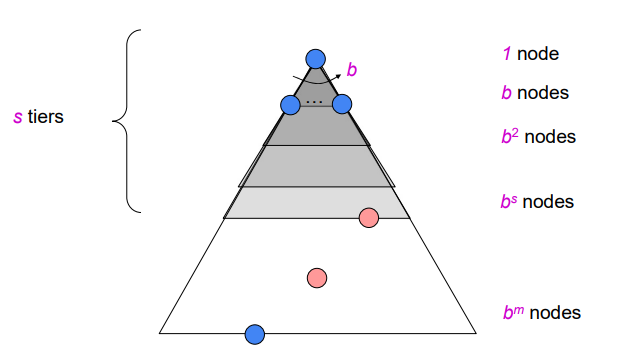
\includegraphics[width = 0.70\linewidth]{Images/32.PNG}
\end{center}
\subsubsection{DFS con approfondimento iterativo (IDDFS)}
L'idea di questo algoritmo è di combinare la complessità spaziale di una DFS con la complessità
temporale di una BFS. L'algoritmo quindi esegue i seguenti passi:
\begin{itemize}
    \item Lancia una DFS con limite di profondità 1. Se non trovi soluzioni... 
    \item Lancia una DFS con limite di profondità 2. Se non trovi soluzioni... 
    \item Lancia una DFS con limite di profondità 3. Se non trovi soluzioni... 
    \item ...
\end{itemize}
\begin{center}
    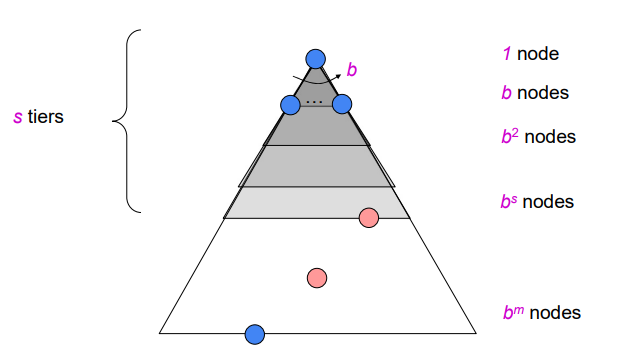
\includegraphics[width = 0.70\linewidth]{Images/32.PNG}
\end{center}
L'algoritmo, tuttavia, non è \textbf{estremamente ridondante?}
Generalmente, la maggior parte del lavoro avviene al \textbf{livello più in profondità esplorato},
quindi l'algoritmo non risulta ridondante. In termini computazionali, se si hanno $b$ possibili scelte per stato
e $s$ è la profondità della soluzione:
\begin{itemize}
    \item \textbf{Spazio}: $\mathcal{O}(s)$
    \item \textbf{Tempo}: $\mathcal{O}(b^s)$
\end{itemize}
\newpage \noindent
Inoltre:
\begin{itemize}
    \item \textbf{Completezza}: quando $s$ è finito
    \item \textbf{Ottimalità}: L'algoritmo è ottimale
\end{itemize}
ricapitolando:
\begin{center}
    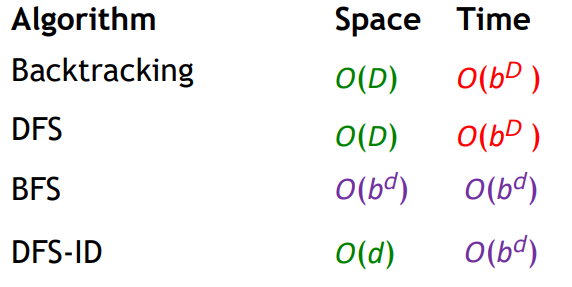
\includegraphics[width = 0.50\linewidth]{Images/34.PNG}
\end{center}

\subsubsection{Il problema della tigre}
Un esempio, molto presente in letteratura, è il cosiddetto "problema della tigre";
ed esso è un esempio di problema \textbf{non risolvibile con gli algoritmi che abbiamo visto fino ad adesso}.
\begin{center}
    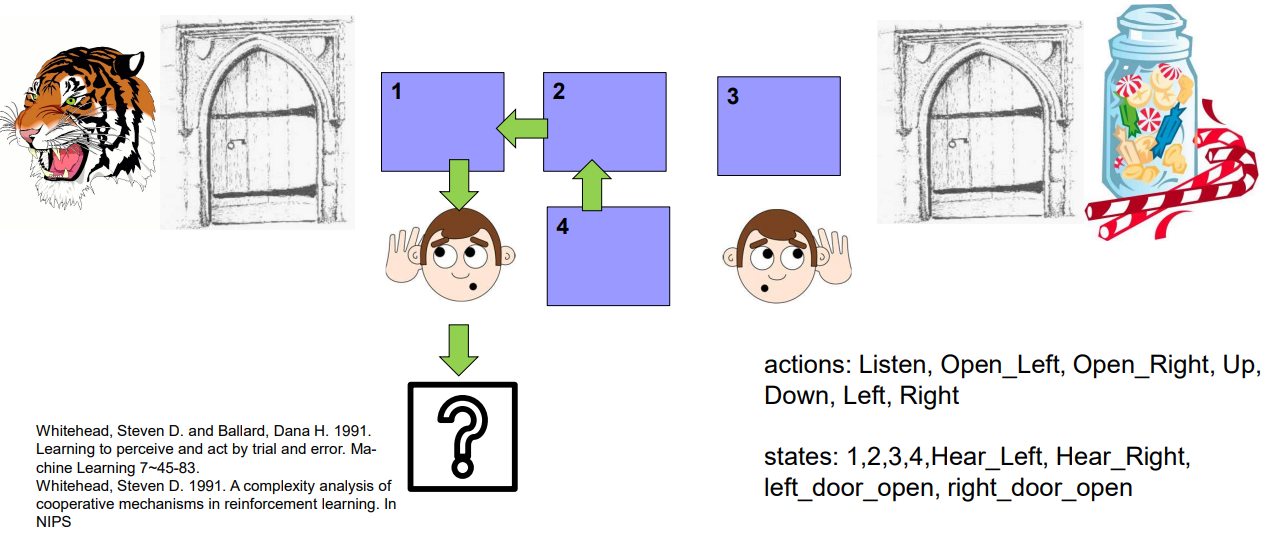
\includegraphics[width = 1\linewidth]{Images/35.PNG}
\end{center}
il problema ha la seguente traccia:
\begin{center}
    Ci si trova in un labirinto formato da stanze. Ogni stanza è collegata alle stanze adiacenti tramite una porta.
    Dietro ad ogni porta ci può essere una tigre oppure delle caramelle, le quali sono il nostro obbiettivo.
    Dopo ogni mossa, la tigre si può muovere in una delle stanze adiacenti a quella in cui si trova correntemente.
    Quale sequenza di azioni bisogna compiere per raggiungere l'uscita del labirinto?
\end{center}
l'agente non sa se dietro una determinata porta c'è la tigre oppure le caramelle; per scoprilo esso può \textbf{ascoltare e sentire se dietro ad una porta sente il rumore provocato dalla tigre}.
Se assumiamo che \textbf{ad ogni stato corrisponda lo stesso risultato} e che quindi una soluzione al problema sia \textbf{un'associazione tra uno stato ed un'azione}; allora in ogni stato possiamo assumere
di conoscere \textbf{quale azioni risolve il problema dato}. In questo caso, tuttavia, \textbf{questa assunzione è errata!} Se, per esempio, nello stato 1 decidiamo di \textbf{ascoltare}, allora abbiamo prodotto
l'associazione "nello stato 1, ascolta"; quindi, se più avanti nella risoluzione del problema torniamo allo stato 1, allora \textbf{ci troveremo ad ascoltare di nuovo}, poiché ad ogni stato viene associata un'azione.
Quindi, quando le conseguenze delle azioni non dipendono solamente da ciò che si può osservare in un determinato istante, non possiamo usare \textbf{gli algoritmi di ricerca che abbiamo visto fino ad ora per risolvere il problema}.
In questo caso bisognerebbe cambiare l'insieme degli stati in modo da \textbf{conservare l'informazione di "aver ascoltato la tigre"}.
Quando andiamo a definire lo spazio degli stati per un problema, ci sono diverse difficoltà da considerare poiché abbiamo la necessità 
che la conseguenza di un'azione dipenda solamente dallo stato in cui si compie l'azione.
Se lo spazio degli stati \textbf{non descrive tutte le informazioni necessarie per risolvere il problema, allora gli algoritmi di ricerca potrebbero entrare in un loop infinito} invece
che convergere alla soluzione.
\subsubsection{Grafo dello spazio degli stati}
Lo spazio degli stati e la funzione di transizione di un problema di ricerca possono anche essere rappresentati
\textbf{mediante un grafo orientato}, che prende il nome di \textbf{grafo dello spazio degli stati}
\begin{center}
    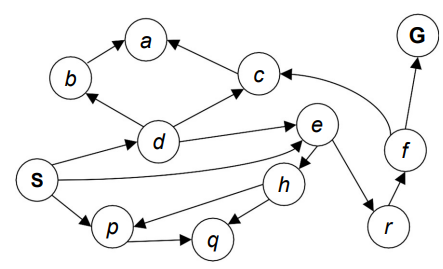
\includegraphics[width = 0.50\linewidth]{Images/36.PNG}
\end{center}
ogni nodo di un grafo dello spazio degli stati rappresenta uno \textbf{stato}, mentre ogni arco rappresenta \textbf{l'azione che dobbiamo intraprendere per passare da un certo stato ad un altro}.
In un grafo dello spazio degli stati \textbf{non ci possono essere stati duplicati!}
Come per l'albero di ricerca, è impossibile, per problemi interessanti, rappresentare in memoria l'intero grafo degli stati.
Un albero di ricerca \textbf{rappresenta l'insieme di percorsi e le soluzioni che sono state studiate fino a quel momento}; una soluzione del problema è quindi un \textbf{cammino dalla radice alla foglia il cui stato soddisfa le condizioni del problema}.
In certi casi, una rappresentazione a grafo dello spazio degli stati è molto più conveniente di un albero, il quale potrebbe risultare di profondità \textbf{infinita}
\begin{center}
    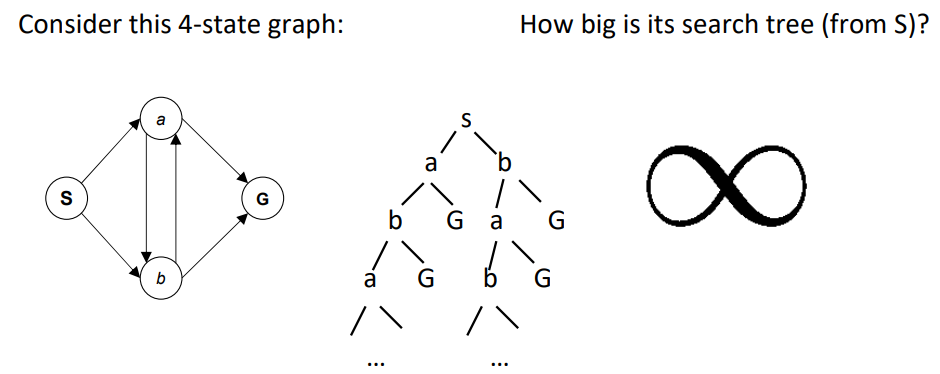
\includegraphics[width = 0.65\linewidth]{Images/37.PNG}
\end{center}
tendenzialmente quindi, un albero di ricerca ha più nodi di un grafo dello spazio degli stati.
\subsubsection{Il problema del costo}
Come abbiamo visto sopra, un problema di ricerca è anche caratterizzato dal \textbf{costo che ogni azione ha per essere intrapresa}.
Come sappiamo, una \textbf{soluzione} è una sequenza di azione che raggiunge uno stato che \textbf{superi il "goal test"} (quindi una soluzione arriva ad una configurazione accettabile del problema).
Una \textbf{soluzione ottima} è la soluzione \textbf{con il costo complessivo minore}.
Poiché diverse azioni, che portano in diversi stati, possono avere diversi costi; cosa può succedere quindi quando si cerca di costruire
un \textbf{cammino di costo minimo} su un grafo che presenta \textbf{degli archi con costo negativo}?
Se esiste un ciclo sul grafo che presenta archi di costo negativo, allora si rischia \textbf{che il cammino di costo minimo abbia costo $-\infty$}.
Per i prossimi algoritmi che presenteremo, assumeremo quindi che ogni arco abbia un costo \textbf{positivo}.
Prima di presentarli facciamo due ulteriori considerazioni:
\begin{itemize}
    \item Un algoritmo che effettua una BFS trova il cammino di costo minimo se e solo se i costi di ogni azione sono uguali
    \item Un algoritmo che effettua una DFS trova il cammino di costo minimo se e solo se i costi di ogni azione sono nulli
\end{itemize}
\subsubsection{Uniform Cost Search (UCS)}
In questo algoritmo, si procede ad esplorare il nodo che ha \textbf{costo minore dall'origine}.
\begin{center}
    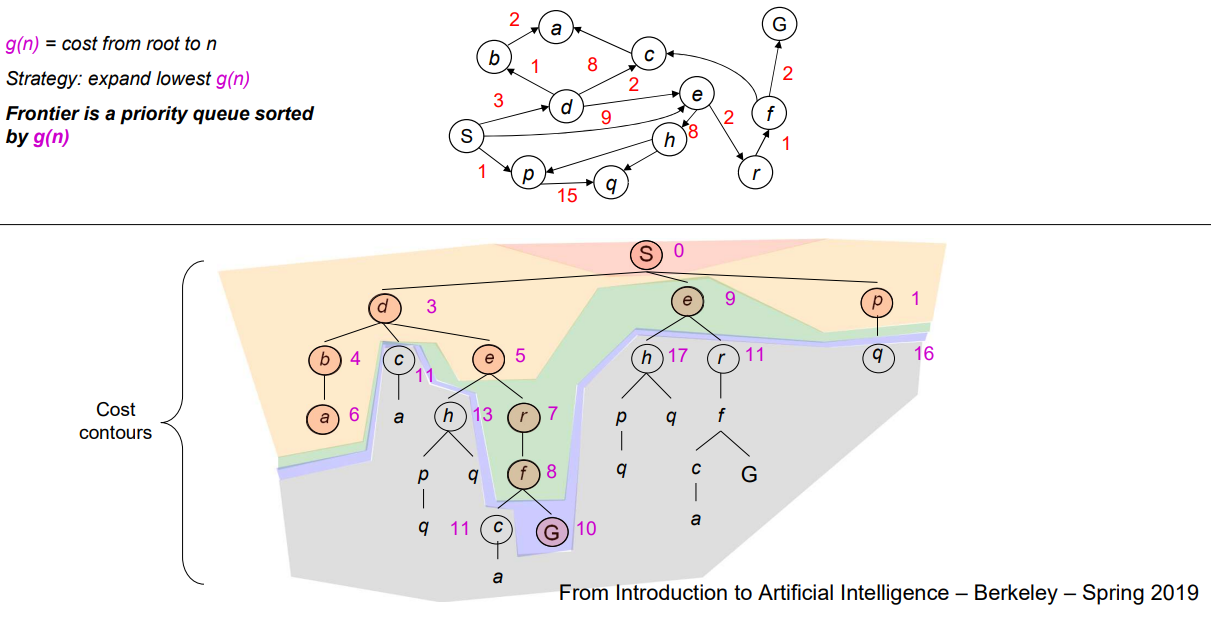
\includegraphics[width = 0.90\linewidth]{Images/38.PNG}
\end{center}
un implementazione di questo algoritmo è quindi la seguente:
\begin{center}
    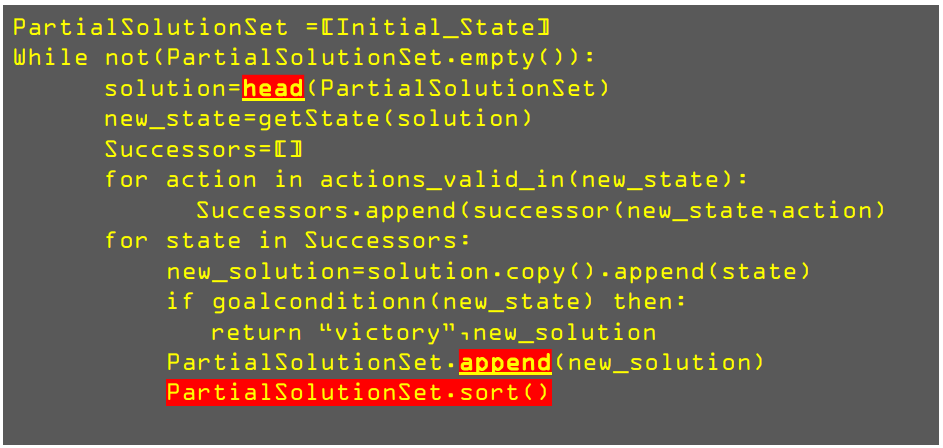
\includegraphics[width = 0.85\linewidth]{Images/39.PNG}
\end{center}
questo algoritmo ha le seguenti proprietà:
\begin{itemize}
    \item Quali nodi espande l'algoritmo?
    \begin{itemize}
        \item Espande tutti i nodi con \textbf{costo minore rispetto alla soluzione meno costosa!}
        \item Se la soluzione costa $C^*$ e gli archi hanno un costo di almeno $\varepsilon$, allora "la profondità effettiva" della soluzione meno costosa è $C^*/\varepsilon$.
    \end{itemize}
    \item \textbf{Completezza}: Assumendo che $C^*$ è finito e $\varepsilon > 0$, allora si!
    \item \textbf{Ottimalità}: L'algoritmo è ottimale
\end{itemize}
In termini computazionali, si ha che, se $b$ è il numero di azioni possibili in ogni stato:
\begin{itemize}
    \item \textbf{Spazio}: $\mathcal{O}(b^{C^*/\varepsilon})$
    \item \textbf{Tempo}: $\mathcal{O}(b^{C^*/\varepsilon})$
\end{itemize}
\begin{center}
    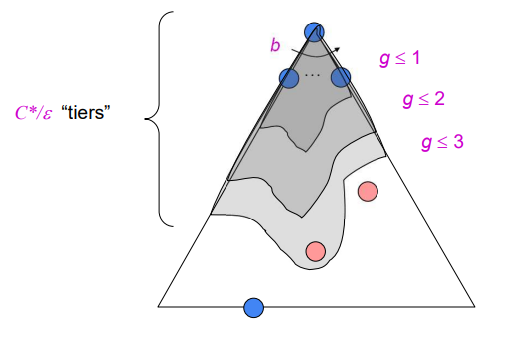
\includegraphics[width = 0.55\linewidth]{Images/40.PNG}
\end{center}
Enunciamo il teorema di \textbf{correttezza} per questo algoritmo:
\begin{Teorema}[Correttezza di UCS]
    Quando uno stato $s$ viene rimosso dalla frontiera e posto tra i nodi esplorati, la sua priorità è $PastCost(s)$, cioè il minimo costo di $s$
\end{Teorema}
\begin{Dimostrazione}
    Se $s$ viene scelto, allora è il nodo che ha \textbf{costo minimo sulla frontiera}; quindi ogni altro cammino ad $s$ sarà più costoso, se i costi sono positivi.
    Per ogni nodo $u$ nella frontiera, si ha che:
    $$PastCost(s) \leq PastCost(u) \leq PastCost(u) + Cost(u,s)$$
    \begin{center}
        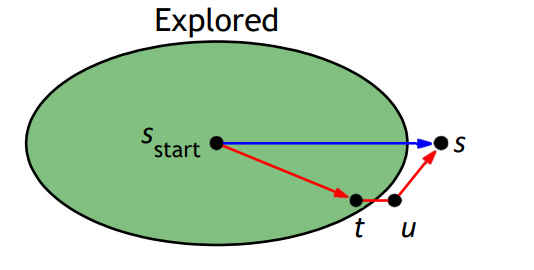
\includegraphics[width = 0.55\linewidth]{Images/41.PNG}
    \end{center}
\end{Dimostrazione}
Tutti gli algoritmi che abbiamo visto fino ad ora sono \textbf{uguali} tranne per \textbf{la gestione dei nodi sulla frontiera}:
\begin{itemize}
    \item Concettualmente, tutte le frontiere sono code di priorità (cioè, collezioni di nodi a cui viene attaccata una certa priorità)
    \item Praticamente, per DFS e BFS, si può evitare l'overhead di $log(n)$ dato da una priority queue usando stack e code
    \item Si può addirittura implementare una variante che prende in input "oggetto di accodamento" (variabile)
\end{itemize}
\subsubsection{Ricerca informata}
Il problema principale di UCS è che \textbf{esplora l'albero degli stati in ogni direzione}; quindi non tiene conto di nessuna informazione
riguardante la \textbf{posizione dell'obbiettivo all'interno dell'albero}.
\begin{center}
    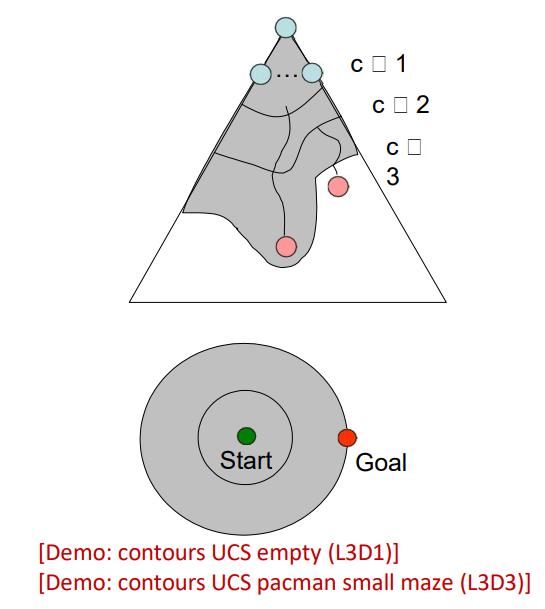
\includegraphics[width = 0.40\linewidth]{Images/42.PNG}
\end{center}
per velocizzare il processo di ricerca, dobbiamo quindi \textbf{guidare la ricerca verso l'obbiettivo}, invece che cercare in tutte le direzioni possibili.
Questo tipo di ricerca viene detto \textbf{ricerca informata}
\begin{center}
    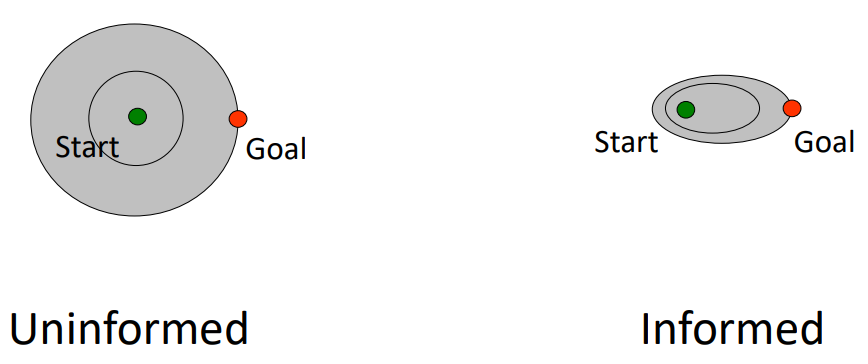
\includegraphics[width = 0.45\linewidth]{Images/43.PNG}
\end{center}
per poter far questo, abbiamo bisogno di inserire più informazione.
In questo caso, tuttavia, l'informazione aggiuntiva non riguarda delle caratteristiche dell'oggetto ma è una \textbf{semplice funzione euristica} che
indica "quanto è facile raggiungere lo stato un obbiettivo da un certo stato".
Queste funzioni euristiche sono \textbf{funzioni dell'obbiettivo}, quindi, per ogni obbiettivo da raggiungere, necessitiamo di una funzione euristica.
Quindi, \textbf{un euristica} è:
\begin{itemize}
    \item Una \textbf{funzione} che \textit{stima} quanto vicino è uno stato all'obbiettivo
    \item Ogni euristica è progettata per un particolare problema di ricerca
    \item Esempi: Manhattan Distance, Euclidean Distance for pathing ecc...
\end{itemize}
Se l'agente impara una certa funzione euristica per un certo obbiettivo; se l'obbiettivo cambio sarà necessario apprendere
una nuova euristica. Un euristica, per funzionare, deve però \textbf{effettuare previsioni minori del valore reale}, cioè deve sottostimare
il costo di raggiungere l'obbiettivo rispetto al costo reale.
\subsubsection{Greedy Search}
Uno degli approcci che utilizza le euristiche viene chiamato \textbf{greedy search}.
L'algoritmo andrà ad esplorare il nodo \textbf{che sembra essere più vicino all'obbiettivo}
\begin{center}
    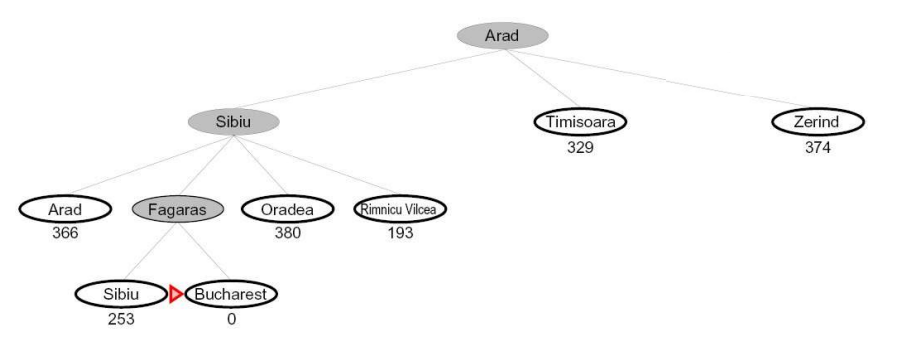
\includegraphics[width = 1\linewidth]{Images/44.PNG}
\end{center}
l'algoritmo è quindi simile ad UCS, ma al posto di esplorare il nodo che ha costo minimo rispetto all'origine,
\textbf{esplora invece il prossimo nodo che ha un costo atteso, quindi un'euristica minima, verso l'obbiettivo}.
La strategia dell'algoritmo è quindi quella di espandere il nodo che \textbf{l'euristica valuta come più vicino all'obbiettivo} (quindi il migliore tra i nodi da esplorare).
L'euristica in questo caso offre, \textbf{per ogni stato dell'albero}, una \textbf{stima della distanza dall'obbiettivo più vicino}.
\begin{center}
    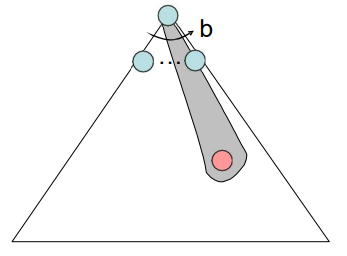
\includegraphics[width = 0.40\linewidth]{Images/45.PNG}
\end{center}
L'algoritmo tuttavia, \textbf{in presenza di un euristica non ottimale}, fatica nel trovare effettivamente una soluzione ottima \textbf{poiché esso non tiene conto del costo totale per raggiungere ogni nodo a partire dalla radice} ma
considera solamente il costo \textbf{per passare da un nodo all'altro}.
\begin{center}
    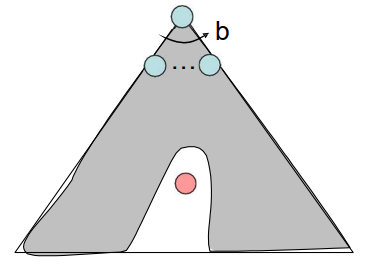
\includegraphics[width = 0.40\linewidth]{Images/46.PNG}
\end{center}
\subsubsection{$A^*$ Search}
L'algoritmo di ricerca $A^*$ combina gli algoritmi UCS e Greedy Search.
Per farlo, assegna ad ogni nodo dell'albero un numero ottenuto sommando i costi del percorso seguito per arrivare fino a quel nodo e la stima del costo che
l'euristica prevede per arrivare all'obbiettivo da quel nodo.
Siano quindi:
\begin{itemize}
    \item $g(n)$ il costo per arrivare dalla radice al nodo $n$
    \item $h^*(n)$ il costo ottimale per arrivare da $n$ all'obbiettivo più vicino
\end{itemize}
L'idea alla base di $A^*$ è quindi la seguente:
\begin{itemize}
    \item Si espande un nodo $n$ che ha maggiore probabilità di essere su un cammino ottimale verso l'obbiettivo
    \item Si espande un nodo $n$ tale che il costo della migliore soluzione che passa per $n$ sia ottimale
    \item Si espande un nodo $n$ con il minor valore di $g(n) + h^*(n)$ 
    \item Solo in rari casi sappiano quanto vale $h^*(n)$, tuttavia potremmo avere una sua \textbf{approssimazione euristica} $h(n)$
    \item $A^* =$ ricerca su un albero con una coda di priorità ordinata rispetto a $f(n) = g(n) + h(n)$
\end{itemize}
\begin{center}
    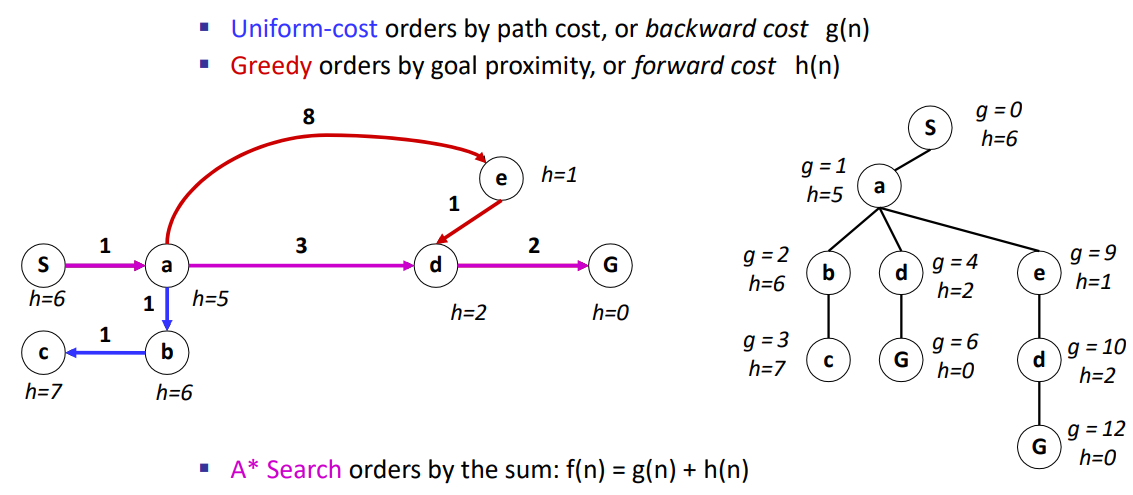
\includegraphics[width =1\linewidth]{Images/47.PNG}
\end{center}
Per fare in modo che \textbf{$A^*$ sia ottimo}, abbiamo bisogno che l'euristica sia \textbf{ottimista rispetto al costo reale}.
Quando si dovrebbe fermare l'algoritmo? Ovviamente, \textbf{non possiamo fermarci quando troviamo il goal} (cioè quando immettiamo nella coda di priorità il nodo), poiché
\textbf{potrebbero esistere dei cammini sul grafo di costo minore di quello correntemente considerato}.
Ci fermiamo quindi solamente quando \textbf{rimuoviamo dalla coda di priorità il nodo goal} (cioè quando lo espandiamo).
In che condizioni $A^*$ è \textbf{ottimale}? Per fare in modo che $A^*$ trovi il cammino di costo minimo, l'euristica che esso usa
deve essere \textbf{ammissibile}:
\begin{itemize}
    \item Un'euristica \textbf{inammissibile} (pessimistica) rompe l'ottimalità dell'algoritmo, poiché non gli permette di esplorare le soluzioni che porterebbero alla soluzione ottima
    \item Un'euristica \textbf{ammissibile} (ottimista) non è mai al di sopra del costo reale
\end{itemize}
Diamo quindi una definizione di euristica ammissibile:
\begin{Definizione}[Euristica ammissibile]
    Un'euristica ammissibile $h$ si dice ammissibile quando
    $$0 \leq h(n) \leq h^*(n)$$
    dove $h^*(n)$ è il reale costo per arrivare all'obbiettivo più vicino
\end{Definizione}
Enunciamo quindi il seguente teorema:
\begin{Teorema} [Ottimalità di $A^*$]
    Si assuma che $A$ sia un noto obbiettivo ottimo, che $B$ sia un nodo obbiettivo sub-ottimale e che $h$ sia un'euristica ammissibile.
    Allora $A$ sarà scelta per l'espansione prima di $B$
\end{Teorema}
\begin{Dimostrazione}
    Immaginiamo che sia $B$ sia alcuni antenati $n$ di $A$ stiano sulla frontiera (oppure che sulla frontiera ci sia $A$ stesso).
    Dobbiamo dimostrare quindi che $n$ sarà scelto per l'espansione prima di $B$.
    Facciamo le seguenti considerazioni:
    \begin{enumerate}
        \item $f(n) \leq f(A)$ poiché:
        \begin{itemize}
            \item La definizione della funzione di costo indica che:
            $$f(n) = g(n) + h(n)$$
            $$f(A) = g(A) + h(A)$$
            \item L'euristica ammissibile sottostima il vero costo di A, quindi $h(A) = 0$
            \item $h(n)$ deve sottostimare il vero costo per arrivare da $n$ ad $A$, quindi $g(n) + h(n) \leq g(A)$,
            quindi:
            $$f(n) \leq f(A)$$
        \end{itemize}
        \item $f(A) < f(B)$ poiché:
        \begin{itemize}
            \item Sappiamo che:
            $$f(A) = g(A) + h(A)$$
            $$f(B) = g(B) + h(B)$$
            \item L'euristica deve sottostimare i veri costi per arrivare ad A e B, quindi:
            $$h(A) = h(B) = 0$$
            \item Poiché abbiamo assunto che $B$ è un obbiettivo sub-ottimale, allora sicuramente:
            $$g(A) < g(B) \Rightarrow f(A) < f(B)$$
        \end{itemize}
    \end{enumerate}
    Quindi tutti gli antenati di $A$ saranno espansi prima di $B$ e $A$ sarà espanso prima di $B$.
    L'algoritmo $A^*$ è quindi ottimo.
\end{Dimostrazione}
\subsubsection{Creare euristiche ammissibili}
Spesso, le euristiche ammissibili non sono altre che \textbf{soluzioni a rilassamenti di un problema}, dove nuove azioni vengono rese ammissibili.
Diamo quindi la seguente definizione:
\begin{Definizione}[Problema rilassato]
    Un problema $P_2$ è una versione rilassata del problema $P_1$ se $\mathcal{A}_2(s) \supseteq \mathcal{A}_1(s)$ per ogni $s$
\end{Definizione}
\begin{Teorema}
    $h_2^*(s) \leq h_1^*(s)$ per ogni $s$, quindi $h_2^*(s)$ è un euristica ammissibile per $P_1$
\end{Teorema}
Quali fattori quindi possiamo considerare quando cerchiamo una buona euristica?
\begin{itemize}
    \item La funzione di successione aiuta? E le azioni?
    \item Cosa succede se si aggiungono/rimuovono casualmente delle azioni da stati casuali? Quali sarebbero le soluzioni risultanti in una funzione euristica ammissibile?
\end{itemize}
Quando si hanno più euristiche tra cui scegliere, esse si possono \textbf{combinare}.
Quali sono quindi i criteri da seguire quando si combinano delle euristiche?
\begin{itemize}
    \item \textbf{Dominanza}: $h_1 \geq h_2$ se $\forall n, h_1(n) \geq h_2(n)$
    Quindi, assumendo che entrambe le euristiche siano ammissibili, si prende quella con il valore più ottimista.
    \item L'euristica nulla non è per niente ottimale (Con $A^*$, ci si ritrova nuovamente con UCS)
    \item L'euristica esatta è buona, ma solitamente troppo costosa
    \item \textbf{Cosa fare se nessuna delle due euristiche domina l'altra?}
    \begin{itemize}
        \item Si forma una nuova euristica prendendo i valori massimi di entrambe:
        $$h(n) = \max\{h_1(n), h_2(n)\} \; \forall n$$
        Il massimo di due euristiche ammissibili è esso stesso ammissibile e domina entrambe.
    \end{itemize}
\end{itemize}
\subsubsection{Euristiche consistenti}
Una ricerca DFS ha il problema che \textbf{si blocca in caso di loop} all'interno dell'albero.
Tuttavia, una DFS risparmia memoria ed è possibile riutilizzarla in altri contesti.
Vogliamo quindi evitare che la DFS espanda gli stessi sotto-alberi.
Come possiamo fare? \textbf{Abbiamo abbastanza informazioni solamente guardando l'albero di ricerca per farlo?}
La strategia di selezione che abbiamo seguito fino ad ora è quella di partire ad espandere i nodi dell'albero che non sono ancora stati espansi;
tuttavia non abbiamo controllato se \textbf{questi nodi sono già presenti nell'albero}. Dobbiamo quindi gestire meglio la struttura dati che utilizziamo
per implementare l'algoritmo.
\begin{center}
    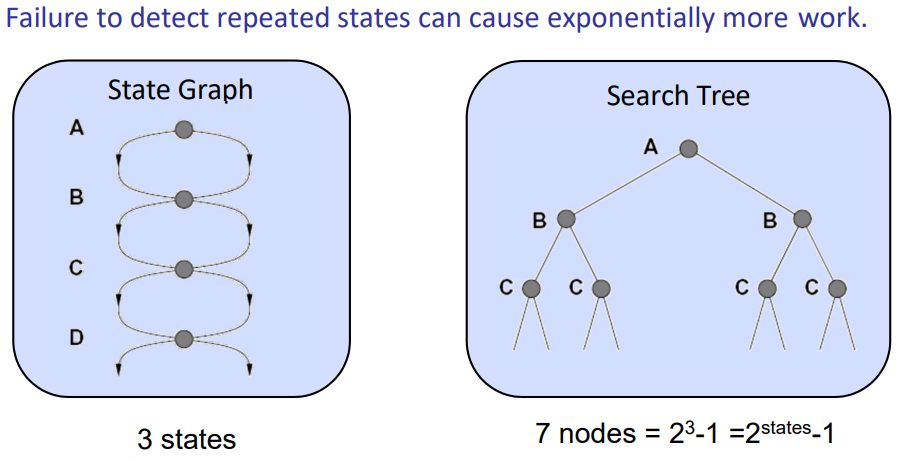
\includegraphics[width =0.90\linewidth]{Images/48.PNG}
\end{center}
Ciò che si fa per evitare questa problematica è passare da algoritmi di ricerca sugli alberi a \textbf{algoritmi di ricerca su grafi}.
L'idea è quindi quella di \textbf{non espandere mai uno stato due volte}.
L'implementazione è quindi la seguente:
\begin{itemize}
    \item Alla ricerca sull'albero si aggiunge un \textbf{insieme degli stati già espansi} ("closed set")
    \item Si espande l'albero di ricerca nodo per nodo, ma... 
    \item Prima di espandere un nodo, ci si assicura che quello stato non sia mai stato espanso prima
    \item Se lo stato è già stato espanso, lo si salta, altrimenti lo si aggiunge al closed set
\end{itemize}
\textbf{IMPORTANTE}: Bisogna immagazzinare il closed set \textbf{come un set}, non una lista. \newline
Questo approccio riesce quindi ad evitare la presenza di loop, tuttavia esso può \textbf{andare a intaccare la completezza e l'ottimalità degli algoritmi di ricerca}.
Facciamo il seguente esempio:
\begin{center}
    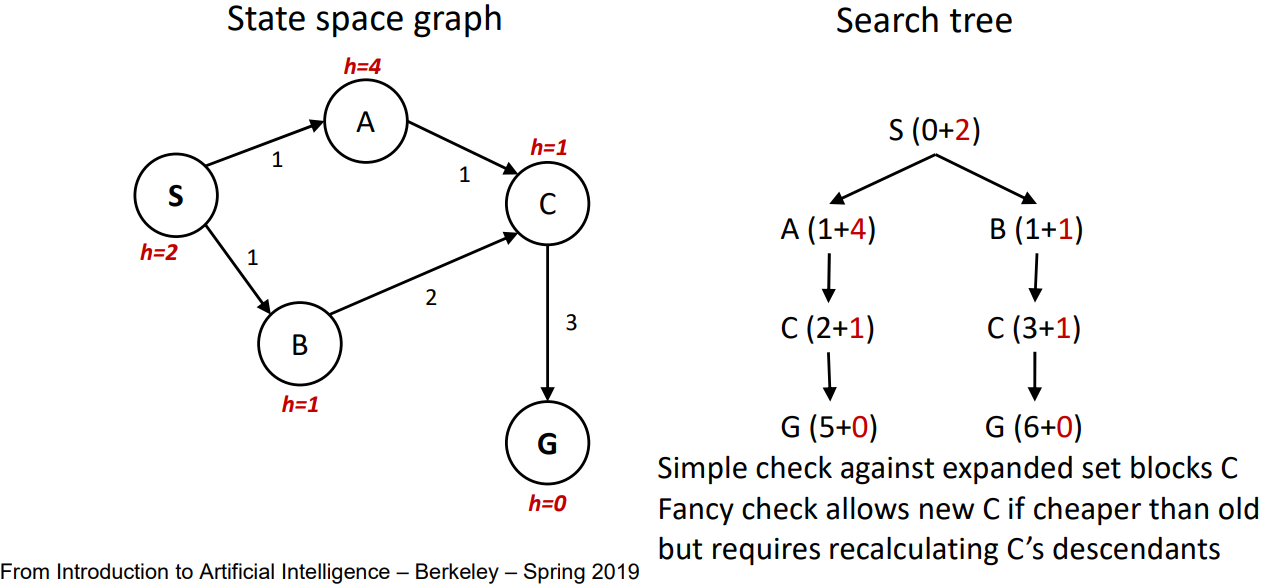
\includegraphics[width =0.90\linewidth]{Images/49.PNG}
\end{center}
come si può vedere, il percorso di costo minimo verrebbe bloccato. Per evitare questo tipo di problematica, abbiamo quindi bisogno di un'\textbf{euristica consistente}:
\begin{itemize}
    \item \textbf{Idea principale}: La stima euristica dei costi deve essere minore o uguale al costo effettivo
    \begin{itemize}
        \item \textbf{Ammissibilità}: Il costo euristico deve essere minore del costo effettivo per arrivare all'obbiettivo:
        $$h(A) \leq h^*(A)$$
        \item \textbf{Consistenza}: Il costo euristico per ogni arco deve essere minore o uguale al costo effettivo per ogni arco:
        $$h(A) - h(C) \leq c(A \; to \; C)$$
        oppure deve rispettare la diseguaglianza triangolare:
        $$h(A) \leq c(A \; to \; C) + h(C)$$
        \textbf{Nota}: $h^*$ necessariamente soddisfa la diseguaglianza triangolare
    \end{itemize}
    \item \textbf{Conseguenze della consistenza}:
    \begin{itemize}
        \item Il valore di $f$ lungo un certo cammino non decresce mai:
        $$h(A) \leq c(A, C) + h(C) \Rightarrow g(A) + h(A) \leq g(A) + c(A,C) + h(C)$$
        \item $A^*$ quindi è ottimale
    \end{itemize}
\end{itemize}
Rendere un euristica consistente però \textbf{non è banale}, poiché bisognerebbe verificarla per tutti gli stati; non possiamo quindi
farlo tramite un approccio "forza bruta", poiché richiederebbe calcolare \textbf{il percorso ottimo all'obbiettivo da ogni singolo stato}.
Quindi, se si ha un'euristica consistente, allora si può direttamente utilizzare $A^*$.
Altrimenti, è necessario avere dei controlli più complessi su quali stati sono già stati visitati.
Per quanto riguarda l'ottimalità di $A^*$ quindi:
\begin{itemize}
    \item \textbf{Tree search}: $A^*$ è ottimo se l'euristica è \textbf{ammissibile}
    \item \textbf{Graph search}: $A^*$ è ottimo se l'euristica è \textbf{consistente}
    \item La consistenza di un'euristica ne implica l'ammissibilità
    \item La maggior parte delle euristiche ammissibili tendono ad essere anche consistenti, specialmente se esse derivano da problemi rilassati
\end{itemize}
Tuttavia, dobbiamo tenere in considerazione che:
\begin{itemize}
    \item $A^*$ mantiene l'intera regione esplorata in memoria, quindi finirà lo spazio per problemi molto complessi
    \item Ci sono varianti che utilizzano meno memoria:
    \begin{itemize}
        \item $IDA^*$ funzione come IDDFS, eccetto che usa una funzione di limite $f$ invece che un limite di profondità
        \item $RBFS$ è un algoritmo DFS ricorsivo che usa una funzione di limite $f$ uguale al miglior cammino alternativo disponibile da uno qualsiasi degli antenati del nodo corrente
        \item $SMA^*$ usa tutta la memoria disponibile per la coda, minimizza quindi il thrashing.
    \end{itemize}
\end{itemize}
\subsection{Classical Planning}
Fino ad adesso, non abbiamo utilizzato tutte le caratteristiche degli stati. Infatti, abbiamo trattato
gli stati come se fossero delle "etichette" per capire se un certo stato fosse già stato esplorato o meno.
I problemi di \textbf{planning} sono simili ai problemi di ricerca nella misura che, per entrambi, \textbf{una soluzione è un insieme di passi sequenziali che permetta di raggiungere uno stato desiderato}.
Un \textbf{planner} accetta un problema e automaticamente computa una sua soluzione. Per farlo, i problemi devono essere codificati in un \textbf{linguaggio indipendente dal dominio} (domain-independent language):
\begin{itemize}
    \item Quali \textbf{azioni} e \textbf{sensori} sono disponibili e come funzionano
    \item Qual'è \textbf{l'obbiettivo} e qual'è \textbf{la situazione iniziale}
\end{itemize}
Nel caso più semplice, abbiamo:
\begin{enumerate}
    \item Una situazione iniziale \textbf{completamene nota}
    \item Gli effetti delle azioni sono \textbf{deterministici}
    \item Non c'è bisogno di \textbf{alcuna percezione}
\end{enumerate}
Questa forma di planning è detta, nel campo dell'IA, \textbf{classical planning}.
Nel caso più generale, le assunzioni sopra vengono \textbf{rilassate}.
In un problema di classical planning, abbiamo:
\begin{itemize}
    \item Uno \textbf{spazio degli stati} discreto e finito $S$
    \item Uno \textbf{stato iniziale noto} $s_0 \in S$
    \item Un insieme $S_G \subseteq S$ di \textbf{stati obbiettivo}
    \item Delle azioni $\mathcal{A}(s) \subseteq A$ applicabili ad ogni $s \in S$
    \item Una \textbf{funzione di transizione degli stati deterministica} $s^j = f(a,s) \; per \; a \in \mathcal{A}(s)$
    \item Un \textbf{costo positivo} per le azioni $c(a, s)$
\end{itemize}
Una \textbf{soluzione} (o \textbf{piano}) è una sequenza di azioni applicabili $a_0, \dots, a_n$ che mappa $s_0$ all'interno di $S_G$, cioè
esiste una sequenza di stati $s_0, \dots, s_{n+1}$ tale che $a_i \in \mathcal{A}(s_i),$ \newline  $s_{i+1} = f(a_i, s_i)$, e $s_{n+1} \in S_G, i = 0,\dots,n$.
Un piano è \textbf{ottimale} se minimizza la \textbf{somma dei costi delle azioni}, cioè
$$\sum_{i=0}^n c(a_i, s_i)$$
Tuttavia, modellare un problema secondo un modello a stati e risolverlo come un problema di ricerca è \textbf{differente} rispetto a modellare il problema come un problema di classical planning.
La differenza viene dall'uso dei \textbf{linguaggi di planning} (STRIPS, PDDL, ecc...) e da una \textbf{rappresentazione più ricca degli stati} (data proprio da questi linguaggi), i quali, in un problema di classical planning, non sono solo
delle label. Si passa inoltre da agenti che hanno una conoscenza basilare dell'ambiente ad \textbf{agenti con una conoscenza dell'ambiente più strutturata}:
\begin{itemize}
    \item Gli agenti \textbf{acquisiscono conoscenza attraverso la percezione, \newline l'apprendimento  e il linguaggio}
    \begin{itemize}
        \item Gli agenti possono rappresentare \textbf{conoscenza sulle conseguenze delle proprie azioni}, quindi si possono utilizzare svariati linguaggi (LISP, Prolog, Logiche di vario tipo, ...) per rappresentare la funzione di transizione ("transition model")
        \item Gli agenti sanno come i loro sensori \textbf{corrispondo allo stato del mondo} ("sensor model"), cioè hanno conoscenza sul come interpretare le percezioni dei propri sensori
        \item Gli agenti conoscono lo \textbf{stato attuale dell'ambiente}
    \end{itemize}
    \item Gli agenti \textbf{possono anche tener traccia delle parti dell'ambiente che attualmente non sta osservando}, quindi possono tener traccia di \textbf{un ambiente parzialmente osservabile}. I linguaggi di planning quindi possono esprimere condizioni più complesse, dove vi è una distinzione fra quello che l'agente osserva in un'istante  e quello che è effettivamente lo stato del mondo.
    \item Gli agenti \textbf{possono formulare piani per raggiungere l'obbiettivo}
\end{itemize}
Gli agenti quindi si avvalgono di una \textbf{base di conoscenza}, cioè di un'\textbf{insieme di frasi scritte in un linguaggio formale}.
La costruzione di un'agente avviene quindi in \textbf{maniera dichiarativa}:
\begin{itemize}
    \item Bisogna \textbf{dirgli oppure fargli apprendere} ciò che ha bisogno di conoscere
    \item Dopodiché, esso può \textbf{chiedersi} cosa fare: le risposte dovrebbero \textbf{derivare dalla base di conoscenza} (KB) 
\end{itemize}
Gli agenti possono essere visti, quindi, \textbf{al livello della conoscenza}, cioè ci si può focalizzare \textbf{su ciò che sanno} indipendentemente da come essi sono implementati.
Un singolo algoritmo di inferenza può rispondere a tutte le domande a cui è possibile rispondere.
\begin{center}
    \includegraphics[width =0.60\linewidth]{Images/50.PNG}
\end{center}
Facciamo un esempio: supponiamo di voler codificare in logica proposizionale una partita di PacMan sulla seguente mappa:
\begin{center}
    \includegraphics[width =0.30\linewidth]{Images/51.PNG}
\end{center}
In questo caso, la maggior parte della base di conoscenza sarebbe occupata da $\mathcal{O}(NT)$ frasi del modello di transizione, con $N$ il numero
di posizioni possibili e $T$ gli istanti temporali. Se ogni frase sono più o meno 10 linee di testo, e se supponessimo $N = 200, T = 400$ allora dovremmo scrivere, più o meno,
800.000 linee di testo, cioè 20.000 pagine.
Questo è dato dal fatto che la logica proposizionale ha una capacità espressiva limitata.
Invece, se decidessimo di usare la logica del primo ordine, avremmo bisogno solamente di un numero $\mathcal{O}(1)$ di frasi del modello di transizione.
Tuttavia, se decidessimo comunque di utilizzare la logica proposizionale, potremmo scrivere un \textbf{agente basato sulla conoscenza} che, ad ogni passo, aggiorni la base di conoscenza e si chieda qual'è la prossima azione da compiere (quindi effettua un'inferenza sulla KB):
\begin{center}
    \includegraphics[width =0.70\linewidth]{Images/52.PNG}
\end{center}
questo tipo di approccio può essere usato anche per i seguenti problemi:
\begin{itemize}
    \item \textbf{Localizzazione} con una mappa e delle percezioni locali 
    \begin{itemize}
        \item Dati una KB iniziale, più una sequenza di azioni e percezioni, dove sono?
    \end{itemize}
    \item \textbf{Costruire una mappa} con un sensore locale
    \begin{itemize}
        \item Data una KB iniziale, più una sequenza di azioni e percezioni, qual'è la mappa?
    \end{itemize}
    \item \textbf{SLAM: Simultaneous Localization and Mapping}
    \begin{itemize}
        \item Localizzazione + Costruire una mappa
    \end{itemize}
    \item \textbf{Planning}
    \begin{itemize}
        \item Data una KB iniziale, più una sequenza di azioni e percezioni, qual'è la sequenza di azioni che mi garantisce di raggiungere l'obbiettivo?
    \end{itemize}
\end{itemize}
Il vantaggio di questo approccio è che, per tutti i problemi precedenti, \textbf{possiamo usare lo stesso algoritmo e la stessa KB}.
Ricapitolando, quindi:
\begin{itemize}
    \item Una possibile architettura par un agente è quella di conoscenza + inferenza
    \item La logica mette a disposizione una maniera formale per codificare la conoscenza
    \item Una semplice KB per PacMan compre lo stato iniziale, il sensor model e il transition model
    \item L'inferenza logica computa le \textbf{relazioni di implicazione} tra le frasi, permettendo che un ampio spettro di compiti possano essere risolti
\end{itemize}
\subsubsection{STRIPS}
STanford Research Institute Problem Solver (STRIPS) è un linguaggio di classical planning.
Un \textbf{problema} in STRIPS è una tupla $P = (F, O, I ,G)$ con:
\begin{itemize}
    \item $F$ l'insieme di tutti gli \textbf{atomi} (variabili booleane)
    \item $O$ l'insieme di tutti gli \textbf{operatori} (azioni)
    \item $I \subseteq F$ l'insieme delle \textbf{situazioni iniziali}
    \item $G \subseteq F$ l'insieme delle \textbf{situazioni obbiettivo}
\end{itemize}
Gli operatori $o \in O$ sono rappresentati combinando:
\begin{enumerate}
    \item l'operazione di aggiunta alla lista degli atomi veri $Add(o) \subseteq F$ (simile alla notazione dei DB relazionali. Se è nella lista, allora è vero)
    \item L'operazione di rimozione dalla lista degli atomi veri $Del(o) \subseteq F$
    \item La lista delle precondizioni $Pre(o) \subseteq F$
\end{enumerate}
Un problema in STRIPS $P$ determina uno \textbf{modello a stati} $S(P)$ dove:
\begin{itemize}
    \item Gli stati $s \in S$ sono \textbf{collezioni di atomi} da $F$
    \item Lo stato iniziale $s_0$ è $I$
    \item Gli stati obbiettivo $s$ sono tali che $G \subseteq s$
    \item Le azioni $a \in \mathcal{A}(s)$ sono operazioni in $O$ tali che $Pre(a) \subseteq s$
    \item Il prossimo stato $s^j = s - Del(a) + Add(a)$
    \item Il costo delle azioni $c(a,s)$ sono tutte 1
\end{itemize}
La \textbf{soluzione (ottima) del problema P} è una \textbf{soluzione (ottima) del problema $S(P)$}.
Le estensioni del linguaggio (negazione, effetti condizionali ecc...) offrono maniere convenienti per esprimere i problemi; alcune sono necessarie per descrivere modelli più ricchi (costi, probabilità, ...).
STRIPS ci permette di descrivere un problema \textbf{indipendentemente dal tempo}.
La lista degli atomi veri definisce, quindi, \textbf{lo stato del problema in un determinato istante}.
La \textbf{lista delle precondizioni} per una determinata azione, invece, definisce quali atomi devono essere veri per poter eseguire l'azione.
Facciamo un esempio:
\begin{center}
    \includegraphics[width =1\linewidth]{Images/53.PNG}
\end{center}
Vediamo ora un'esempio più complesso: supponiamo che un robot si trovi in un ambiente formato da due stanze.
Il robot deve trasportare due pacchi dalla stanza $A$ alla stanza $B$. La codifica in STRIPS del problema è quindi la
seguente:
\begin{center}
    \includegraphics[width =1\linewidth]{Images/54.PNG}
\end{center}
In questo caso, abbiamo quindi un numero di stati possibili di $2^8$.
Tuttavia, questa codifica presenta molte ripetizioni. Possiamo quindi usare delle \textbf{variabili} per 
definire in modo più compatto il problema. L'introduzione di variabili necessita inoltre che si possano definire
i \textbf{tipi di queste variabili}. Il problema quindi diventa:
\begin{center}
    \includegraphics[width =1\linewidth]{Images/55.PNG}
\end{center}
\newpage
\subsubsection{PDDL}
Il \textbf{Planning Domain Description Language} (PDDL) è una versione avanzata di STRIPS e si configura come una sintassi standard per i problemi di classical planning.
Sviluppato per la International Planning Competition(IPC), è un linguaggio che continua ad evolversi sin dalla sua creazione, nel 1998.
Durante l'IPC, i pianificatori vengono valutati su \textbf{problemi da loro non ancora visti} codificati in PDDL
\begin{center}
    \includegraphics[width =0.50\linewidth]{Images/56.PNG}
\end{center}
PDDL specifica una sintassi per i problemi $P = (F,I,O,G)$ e supporta STRIPS, variabili, tipi e molto altro.
I problemi in PDDL sono specificati in due parti:
\begin{itemize}
    \item \textbf{Dominio}: Contiene azioni e gli \textbf{schemi degli atomi}, oltre che ai \textbf{tipi degli argomenti}
    \item \textbf{Istanza}: Contiene la \textbf{situazione iniziale, l'obbiettivo} e le \textbf{costanti} (oggetti) per ogni tipo
\end{itemize}
Queste due parti, in PDDL, si trovano in due file separati, in modo da facilitare \textbf{la creazione di diverse istanze per lo stesso problema}.
\begin{center}
    \includegraphics[width =1\linewidth]{Images/57.PNG}
\end{center}
In PDDL, \textbf{i parametri di un'azione devono coprire sia le precondizione che gli effetti}; quindi sono le variabili che vanno utilizzate dentro un'azione
per crearne una completa.
Come facciamo però a risolvere un problema di classical planning?
Il planning è una delle aree più vecchie dell'IA; quindi molte idee sono state provate.
Ciò che si può fare, utilizzando questi linguaggi, è impiegare una vasta gamma di ragionatori per risolvere il problema; questo insieme è più ricco rispetto
a quello dei ragionatori che effettuano una ricerca su grafo poiché i primi possono sfruttare la struttura dello spazio degli stati.
I due metodi classici principali per risolvere problemi di classical planning sono:
\begin{itemize}
    \item Pianificazione come \textbf{ricerca euristica}; questo metodo è ispirato a ciò che abbiamo già detto sulle euristiche
    \item Pianificazione come \textbf{SAT}, cioè si trasforma il piano in un problema di soddisfacimento di vincoli, dove bisogna riuscire a definire il valore di tutte le variabili indefinite.
\end{itemize}
Questi metodi sono in grado di risolvere problemi caratterizzati da un spazio degli stati di dimensione considerevole.
Ovviamente, alcuni problemi sono intrinsecamente difficili, e quindi, per essi, i \textbf{pianificatori generali e indipendenti dal dominio} non saranno
probabilmente in grado di raggiungere le performance di \textbf{metodi specializzati}.
\subsubsection{Pianificazione come ricerca euristica}
L'idea della pianificazione come ricerca euristica è quella di \textbf{sfruttare la corrispondenza tra i modelli a stati (classici) e i grafi orientati}:
\begin{itemize}
    \item I \textbf{nodi} del grafo rappresentano gli \textbf{stati} $s$ del modello
    \item Gli archi $(s, s^j)$ catturano la transizione corrispondente nel modello con lo stesso costo
\end{itemize}
Nella formulazione di una pianificazione come ricerca euristica, il problema $P$ è risolto da degli \textbf{algoritmi di path-finding} su un grafo
associato con il modello $S(P)$, con un'\textbf{euristica} derivata automaticamente da $P$.
Uno sviluppo chiave nel campo del planning, avvenuto negli anni '90, è l'estrazione automatica di \textbf{funzioni euristiche} per guidare la ricerca dei piani (quindi di una soluzione).
L'euristica verrà derivata dal \textbf{rilassamento del problema} dove le \textbf{azioni di cancellazione dalla lista non hanno alcun effetto}. Viene quindi
eliminata la possibilità di rendere falso un atomo. Questo rilassamento viene detto \textbf{delete-relaxation}.
Siano quindi $P(s)$ il problema $P$ con $s$ come suo stato iniziale, $P^+$ la sua delete-relaxation e $h^*_P(s)$ il \textbf{costo ottimale} per risolvere $P$ da $s$.
Allora, \textbf{l'euristica} $h(s)$ potrebbe essere impostata a:
$$h(s) := h_P^+(s)$$
tuttavia, questo non \textbf{funziona computazionalmente}: risolvere $P^+(s)$ in maniera ottimale è difficile quanto risolvere $P(s)$ in maniera ottimale (il problema è NP-Completo).
Dall'altra parte, seppur risolvere il rilassamento $P^+(s)$ ottimamente sia difficile, \textbf{trovare una sua soluzione, non necessariamente ottimale, è semplice}.
Poiché in questo caso viene rimossa la possibilità di rimuovere atomi dalla lista, ciò che si può fare è eseguire \textbf{tutte le azioni eseguibili in un determinato momento} e quindi
vedere quali sono gli \textbf{stati raggiungibili al prossimo passo} e così via fino a non ottenere tutti gli elementi del goal nella lista.
Ciò quindi da una misura della distanza tra un certo stato e lo stato finale; che è un euristica \textbf{ottimistica}. Si può quindi prendere quest'euristica e usarla
per effettuare una ricerca informata (es. con $A^*$).
In realtà, la procedura che effettivamente si adopera comprende anche una fase di "back-tracking", dove si vanno a cancellare \textbf{tutte le azioni inutili}, andando quindi a semplificare
lo spazio degli stati. Un'euristica ammissibile per $h(s)$ per il problema rilassato $P^+$ è quindi l'euristica $h_{max}$, definita come segue:
\begin{itemize}
    \item \textbf{Idea chiave}: I problemi STRIPS \textbf{delete-free} sono \textbf{completamente decomponibili}
    \item Se il piano $\pi_1$ arriva al goal $G_1$ e il piano $\pi_2$ arriva al goal $G_2$, allora il piano $\pi_1, \pi_2$, dove $\pi_2$ segue $\pi_1$, risolve sia il goal $G_1$ che il goal $G_2$
    \item L'osservazione suggerisce la seguente \textbf{procedura iterativa} sopra tutti gli atomi in $P^+(s)$:
    \begin{enumerate}
        \item L'atomo $p$ è \textbf{raggiungibile} in 0 passi se $p \in s$
        \item L'atomo $p$ è \textbf{raggiungibile} in $i + 1$ passi se non è raggiungibile in $i$ passi o meno, ed esiste \textbf{un'azione} $a_P$ in $P$ tali che le \textbf{precondizioni} $p_i$ di $a_P$ sono raggiungibili in $i$ passi o meno        
    \end{enumerate}
    \item \textbf{Affermazioni}:
    \begin{itemize}
        \item La procedura sopra riportata termina in un numero di passi limitato dal numero di atomi; cioè quando non vi sono più atomi raggiungibili
        \item Se l'atomo $p$ non è raggiungibile, allora si può mostrare che non esiste un piano per raggiungere $p$ in $P$
    \end{itemize}
    \item \textbf{Proprietà}:
    \begin{itemize}
        \item $h(s)$ posta al numero di passi richiesti per raggiungere \textbf{tutti gli atomi obbiettivo} è un'\textbf{euristica ammissibile}. Viene chiamata \textbf{euristica massima} oppure $h_{max}$
    \end{itemize}
\end{itemize}
L'euristica $h = h_{max}$ è \textbf{ammissibile}, ma non è particolarmente \textbf{informativa}.
Anche l'euristica $h(s) = 0$ è \textbf{ammissibile}, ma è completamente \textbf{poco informativa}.
Delle euristiche più informative possono essere ottenute da un \textbf{piano} $\pi(s)$ per il rilassamento $P^+(s)$, che viene chiamato \textbf{piano rilassato}.
Un piano rilassato $\pi(s)$ viene ottenuto \textbf{concatenando a ritroso} partendo dagli obbiettivi e utilizzando le azioni $a_P$, identificate dalla \textbf{procedura di raggiungibilità}, che rendono raggiungibili i goal.
La procedura di raggiungibilità è definita come segue:
\begin{center}
    $\pi(s)$ contiene l'azione $a_p$ per ogni obbiettivo $p$ in $P$, $p \in s$, e un'azione $a_q$ per ogni precondizione $q$ dell'azione $\pi(s)$, $q \in s$
\end{center}
\begin{Nota}
    Qui le slide hanno degli artefatti??? La procedura potrebbe essere sbagliata!
\end{Nota}
L'euristica viene quindi impostata a $|\pi(s)|$, cioè il numero di azioni del piano rilassato.
Quest'euristica viene chiamata \textbf{piano rilassato} $h$ o $h_{FF}$; tuttavia, seppur sia \textbf{informativa} (è piuttosto accurata), essa \textbf{non è ammissibile}.
\subsection{Probabilistic Planning}
WIP
\section{Approcci simbolici: basi di conoscenza e ragionamento automatico}
WIP
\section{Approcci sub-simbolici: Machine Learning}
Due fattori importanti che hanno portato a importanti risultati nel campo dell'intelligenza artificiale sono:
\begin{itemize}
    \item \textbf{La crescita della potenza computazionale} dei dispositivi (specialmente le GPU e addirittura la nascita di dispositivi dedicati, es. TPUs)
    \item \textbf{La crescente disponibilità di dati} (specialmente foto, video ma anche testo in lingue differenti). In particolare, questo tipo di dati sono \textbf{annotati}, quindi contengono metadati che ne descrivono il contenuto.
\end{itemize} 
Le reti neurali non erano implementabili fino alla metà degli anni'80. Grazie al presentarsi delle condizioni sopra riportare, divenne quindi plausibile
\textbf{creare delle reti neurali profonde}. Un'esempio è \textbf{ImageNet}, un database di immagini annotate secondo la \textbf{gerarchia WorldNet}, la quale non è un'ontologia assiomatica, ma è un tesauro con relazioni sia \textbf{tassonomiche} che
\textbf{mereologiche} ("parte di"). ImageNet fu strumentale alla creazione delle prime reti neurali profonde.
\subsection{Introduzione al Machine Learning}
\begin{center}
    \includegraphics[width =0.95\linewidth]{Images/58.PNG}
\end{center}
\textbf{Machine Learning} è in realta un termine ombrello che racchiude sotto di se diversi tipi di apprendimento automatico.
Diamo una breve descrizione delle tecniche illustrate sopra:
\begin{itemize}
    \item \textbf{Apprendimento supervisionato}: Si sviluppa un modello predittivo basato sia sui dati in input che sui dati in output. Per andare ad analizzare dati non noti bisogna quindi avere una base esperienziale di dati noti; così che il modello possa associare un output plausibile al dato.
    \begin{itemize}
        \item \textbf{Classificazione}: Il modello riconosce l'appartenenza del dato ad una certa classe
        \item \textbf{Regressione}: Dati in input dei dati numerici, il modello darà in output un dato numerico che "si avvicina" al valore effettivo dato da quelle condizioni
    \end{itemize}
    \item \textbf{Apprendimento non supervisionato}: In questo tipo di apprendimento, il modello ha solamente il \textbf{dato in input}; esso quindi deve interpretare l'input e svolgere una mansione.
    \begin{itemize}
        \item \textbf{Clustering}: Il modello, analizzando i dati in input, trova dei raggruppamenti a cui le diverse parti dell'input appartengono
    \end{itemize} 
\end{itemize}
Tuttavia, come si può notare dallo schema, la situazione è ben più complessa rispetto all'elenco puntato sopra.
Inoltre, che relazione ha tutto questo con la statistica? Il deep learning dove si colloca in questo schema?
Facciamo quindi un passo indietro e chiediamoci la seguente domanda: qual'è la differenza tra la \textbf{programmazione tradizionale} e la \textbf{programmazione di modelli di apprendimento automatico}?
\begin{center}
    \includegraphics[width =0.65\linewidth]{Images/59.PNG}
\end{center}
\begin{itemize}
    \item \textbf{Programmare} è essenzialmente scrivere le operazioni che un esecutore automatico deve seguire per risolvere un qualche problema. Ciò significa che un programma tradizionale ha \textbf{come input dei dati} e darà in \textbf{output dei dati}.
    Tradizionalmente, un programmatore deve esplicitamente definire le operazioni che la macchina dovrà eseguire, cioè deve definire \textbf{le regole che l'esecutore dovrà seguire}.
    \item All'interno di alcune tecniche di apprendimento automatico, il programmatore \textbf{studia il problema} e seleziona un \textbf{algoritmo automatico} che, analizzando i dati, automaticamente produce un programma che risolverà il problema. Un \textbf{algoritmo di Machine Learning} quindi avrà in \textbf{input dei dati} e ritornerà in \textbf{output un programma}.
\end{itemize}
Ovviamente, entrambi i processi sono \textbf{iterativi}; ciò permette la gestione di errori e di risultati che non considerati "abbastanza buoni".
\subsubsection{Introduzione all'apprendimento supervisionato}
Nell'\textbf{apprendimento supervisionato}, i dati di addestramento che vengono dati in pasto all'algoritmo includono le \textbf{soluzioni desiderate}, chiamate \textbf{labels} (etichette).
\begin{itemize}
    \item Esse possono essere \textbf{categorie} (es. SPAM / NOT SPAM) nei \textbf{modelli di classificazione}. La supervisione, quindi, \textbf{è l'avere degli esempi con un'etichettatura}. Ovviamente, gli esempi devono essere in \textbf{numero sufficiente} e devono avere una \textbf{buona rappresentanza delle varia classi}.
    \item Oppure, possono essere \textbf{valori numerici}, dove si cerca di \textbf{apprendere una funzione non nota}, nei \textbf{modelli regressivi} 
\end{itemize}
\begin{center}
    \includegraphics[width =0.65\linewidth]{Images/60.PNG}
\end{center}
\subsubsection{Introduzione all'apprendimento non supervisionato}
Nell'\textbf{apprendimento non supervisionato}, i dati \textbf{non sono etichettati!}
Alcune tipiche mansioni in quest'area sono:
\begin{itemize}
    \item \textbf{Clustering}: Algoritmi che provano a individuare modi di \textbf{raggruppare istanze} all'interno del dataset secondo sia le loro \textbf{caratteristiche} sia le \textbf{caratteristiche dell'intero dataset}.
    \item \textbf{Dimensionality Reduction}: I dati possono essere caratterizzati da un numero molto elevato di caratteristiche; ciò li rende quindi molto difficili da gestire e visualizzare. Quindi, ha, a volte, senso ridurre il \textbf{numero di dimensioni} (cioè il numero di caratteristiche) \textbf{limitando la perdita di informazione}. Questo approccio è molto spesso \textbf{ancillare} ad altre tecniche.
    \item \textbf{Anomaly Detection}: I dati rappresentano un \textbf{singolo insieme di individui "regolari"} e il sistema deve imparare a discriminare i dati che appartengono a questo insieme da quelli non contenuti in esso, cioè dai dati che \textbf{non sono conformi ad una certa struttura dell'insieme}, essa stessa implicata dai dati.
\end{itemize}
\begin{center}
    \includegraphics[width =0.65\linewidth]{Images/61.PNG}
\end{center}
\begin{center}
    \includegraphics[width =0.50\linewidth]{Images/62.PNG}
\end{center}
\subsubsection{Altre classi di apprendimento automatico}
Altre classi di apprendimento automatico sono:
\begin{itemize}
    \item \textbf{Apprendimento semi-supervisionato}: Questo approccio gestisce \textbf{dati di addestramento parzialmente etichettati}. Solitamente, i dataset in cui viene impiegato questo approccio hanno \textbf{una mole molto elevata di dati non etichettati} e una \textbf{piccola quantità di dati etichettati}.
    Questo approccio tipicamente combina algoritmi supervisionati e non supervisionati.
    \item \textbf{Apprendimento per rinforzo}: Questo approccio è molto differente da quelli visti fino ad ora. In questo caso, l'agente viene posto all'interno di un ambiente, del quale conosce \textbf{quali azioni sono disponibili}, ed esso apprende \textbf{essenzialmente tramite un processo di "trial-and-error"}, visto che l'ambiente
    mette a sua disposizione delle \textbf{percezioni} e un \textbf{valore di ricompensa} associato alla precedente azione scelta dall'agente.
\end{itemize}
\subsubsection{Batch Learning vs Online Learning}
Un approccio di ML \textbf{non necessariamente migliora costantemente le proprie performance}.
Per esempio, la figura 1.2 di questa sezione \textbf{non descrive un caso in cui la soluzione "lanciata" viene revisionata}.
La revisione della soluzione dopo il lancio è \textbf{un approccio possibile}:
\begin{center}
    \includegraphics[width =0.65\linewidth]{Images/63.PNG}
\end{center}
tuttavia, l'aggiungere dati \textbf{non necessariamente porterà ad un aumento delle prestazioni del modello}.
Più precisamente, l'addestramento può avvenire secondo le seguenti modalità:
\begin{itemize}
    \item \textbf{Batch learning}: In questo approccio, il modello è addestrato su \textbf{tutti i dati al momento disponibili}
    \begin{itemize}
        \item Ciò, generalmente, richiede molto tempo e molte risorse computazionali, quindi è \textbf{tipicamente svolto offline}
    \end{itemize}
    \item \textbf{Online learning}: In questo approccio, il sistema viene addestrato dandogli in pasto \textbf{delle istanze di dati in maniera sequenziale}, o individualmente o in \textbf{piccoli gruppi}, detti "\textbf{mini-batches}". Gli algoritmi
    di online learning possono anche essere utilizzati per \textbf{addestrare modelli su dataset numerosi} che non riescono a rientrare all'interno della memoria principale di una singola macchina.
    \begin{itemize}
        \item È necessario inoltre definire \textbf{quanto velocemente il modello debba adattarsi alle modifiche nei dati} (\textbf{learning rate}) e quanto il dato nuovo sia rilevante.
    \end{itemize}
\end{itemize}
\begin{center}
    \includegraphics[width =0.70\linewidth]{Images/64.PNG}
\end{center}
\subsubsection{Necessità dell'addestramento di un modello}
Nel machine learning, \textbf{è sempre necessario che vi sia una complessa fase di addestramento del modello?}
La risposta è \textbf{no}. Nelle tecniche non supervisionate, è piuttosto frequente che \textbf{non vi sia una fase di addestramento}, ma semplicemente una fase di \textbf{analisi del dataset}.
Un approccio che non necessita di addestramento è quello del \textbf{instance-based learning}, il quale rappresenta un modo di \textbf{classificare dati basandosi sulla distanza dai dati vicini o sulla similarità}.
\begin{center}
    \includegraphics[width =0.75\linewidth]{Images/65.PNG}
\end{center}
\subsubsection{Criticità della valutazione dei modelli}
Nelle sezioni precedenti, abbiamo parlato di poter \textbf{dimostrare} delle affermazioni oppure di poter \textbf{trovare un valore ottimo}.
Negli approcci di ML, \textbf{è molto difficile che si sia in grado di dimostrare certe affermazioni}; diventa quindi \textbf{imperativo valutare i risultati di un modello},
quindi di discutere quanto essi siano "buoni" e quando e come falliscono. Tutti gli approcci visti fino ad ora hanno una base statistica e richiedono una valutazione dei risultati, le quali
non hanno necessariamente il \textbf{grado di forza che ha una dimostrazione} e quindi sono soggette sempre ad una costante verifica.
La valutazione dei risultati ci permette inoltre di \textbf{accorgerci di eventuali bias del modello}, dati anche da una possibile \textbf{sotto-rappresentazione di certe categorie}.
Le sfide quindi nell'ambito del ML sono:
\begin{itemize}
    \item Quantità di dati di addestramento insufficienti
    \item Dati di addestramento non rappresentativi
    \item Dati di scarsa qualità
    \item Presenza di caratteristiche irrilevanti
    \item Overfitting/Underfitting dei dati di addestramento
\end{itemize}
\begin{center}
    \includegraphics[width =0.80\linewidth]{Images/66.PNG}
\end{center}
\begin{center}
    \includegraphics[width =0.80\linewidth]{Images/67.PNG}
\end{center}
\newpage
\subsection{Apprendimento supervisionato}
Nell'apprendimento supervisionato abbiamo a disposizione una serie di \textbf{esempi} (record, casi, istanze, ecc...).
Diamo quindi delle definizioni più precise:
\begin{itemize}
    \item \textbf{Dati}: Una serie di "record" (anche chiamati esempi, istanze o casi) descritti da:
    \begin{itemize}
        \item \textbf{k attributi} $A_1, \dots, A_k$
        \item \textbf{Una classe} (se parliamo di classificatori): ogni esempio è etichettato con un classe definita a priori
    \end{itemize}
    \item \textbf{Obbiettivo}: Apprendere un \textbf{modello di classificazione} dai dati che possa essere usato per prevedere le classi di nuovi casi/istanze.
\end{itemize}
Se l'output $a$ non appartiene a un \textbf{insieme discreto}, ma è piuttosto un \textbf{valore numerico} (sia discreto che continuo), allora parliamo di \textbf{regressione invece che di classificazione}.
Il resto della discussione rimane invece praticamente uguale.
\begin{center}
    \includegraphics[width =0.80\linewidth]{Images/68.PNG}
\end{center}
Quali sono quindi le differenze con l'apprendimento non supervisionato?
\begin{itemize}
    \item \textbf{Apprendimento supervisionato}: La classificazione è vista come un apprendimento supervisionato dagli esempi
    \begin{itemize}
        \item \textbf{Supervisione}: I dati (osservazioni, misure, ecc...), sono etichettati con classi predefinite. È come se un "insegnate" dia le classi al modello (\textbf{supervisione})
        \item Anche i dati di test vengono classificati in queste classi
    \end{itemize}
    \item \textbf{Apprendimento non-supervisionato} (clustering): Le etichette di classe dei dati \textbf{non sono noti a priori}. Dato quindi un insieme di dati, il compito è quello di stabilire l'esistenza di classi o di \textbf{raggruppamenti} all'interno del dataset
\end{itemize}
\newpage
\noindent
Il flusso di lavoro dell'apprendimento supervisionato generalmente prevede le seguenti fasi:
\begin{enumerate}
    \item \textbf{Apprendimento (addestramento)}: Viene appreso un modello usando i \textbf{dati di addestramento}
    \item \textbf{Testing}: Si testa il modello utilizzato \textbf{dati di test non visti durante la fase di addestramento} per stabilire l'accuratezza del modello.
    Un modo per stimare l'accuratezza di un modello può essere la seguente:
    $$Accuracy = \frac{\textrm{Number of correct classifications}}{\textrm{Total number of test cases}}$$
\end{enumerate}
\begin{center}
    \includegraphics[width =0.80\linewidth]{Images/69.PNG}
\end{center}
È necessario notare che \textbf{i dati che vengono utilizzati per testare il modello non devono contenere dati che sono stati utilizzati per addestrarlo}.
L'assunzione di base che ci permette di adottare questo tipo di approccio è la seguente: \newline
\textbf{ASSUNZIONE}: La distribuzione degli esempi (quanti sono appartenenti alle diverse  classi? Ogni classe è rappresentata sufficientemente? E in che proporzione, ed essa è ragionevolmente vicina al mondo reale?) usati nell'addestramento è \textbf{identica} alla distribuzione dei casi di test (inclusi gli esempi futuri mai osservati prima). Cioè, che i dati
del dataset \textbf{siano rappresentativi di come sono davvero i dati nel mondo reale}. \newline
Nella pratica, questa assunzione è \textbf{spesso violata in una certa misura}. Ampie violazioni di questa assunzione, chiaramente, risulteranno in \textbf{una scarsa accuratezza di classificazione}.
Per raggiungere una buona accuratezza sui dati di test, i dati di addestramento devono essere \textbf{sufficientemente rappresentativi}.
\subsubsection{Induzione di alberi di decisione}
Gli alberi di decisione sono una tecnica nota ed utilizzata ai fini di \textbf{classificazione}:
\begin{itemize}
    \item Su dati tabellari, la loro accuratezza è molto competitiva con altri metodi di classificazione
    \item Sono molto efficienti
    \item Su altri tipi di dati, gli alberi di decisione invece risultano meno accurati o efficienti rispetto ad altri approcci
\end{itemize}
La tecnica che andremo a discutere \textbf{costruisce un albero}, il quale avrà sui nodi dei \textbf{test sugli attributi di un nuovo individuo} e che ci permetterà, navigando dalla radice alla foglia, di determinare la \textbf{classe da assegnare ad esso}.
La particolarità di questo albero è ispezionabile, leggibile è può essere \textbf{trasformato in regole del tipo if-then}. L'albero quindi è "spiegabile", cioè è interpretabile ed è possibile capire, da esso, come il modello effettua la classificazione. Non tutti gli algoritmi
producono un modello "spiegabile". Facciamo un esempio di albero di decisione usando la tabella sopra:
\begin{center}
    \includegraphics[width =0.80\linewidth]{Images/70.PNG}
\end{center}
i nodi dell'albero sono associati ad attributi della tabella. In base al tipo di dato, \textbf{il fattore di ramificazione può essere differente}.
Gli alberi di decisione, tuttavia, \textbf{non sono unici}; infatti un albero equivalente e più semplice rispetto a quello sopra è il seguente:
\begin{center}
    \includegraphics[width =0.40\linewidth]{Images/71.PNG}
\end{center}
vogliamo quindi trovare l'albero decisionale \textbf{più piccolo e più accurato possibile}, poiché esso avrà prestazioni migliori e risulterà più facile da comprendere.
Tuttavia, trovare un albero ottimale è un problema \textbf{NP-Completo}; quindi tutti i correnti algoritmi di costruzione di alberi decisionali sono \textbf{algoritmi euristici}; quindi sono algoritmi che non garantiscono l'ottimalità
ma hanno \textbf{ottime proprietà computazionali} (tempo di esecuzione e utilizzo di memoria). Per loro struttura, invece, fare un'inferenza su un albero decisionale ha un \textbf{costo logaritmico rispetto al numero dei nodi}, quindi effettuare una classificazione
tramite un albero decisionale ha un costo relativamente basso.
Come abbiamo detto, un albero di decisione può essere convertito in un \textbf{insieme di regole}; in particolare, ognuna di esse rappresenterà un \textbf{cammino dalla radice ad una foglia}.
Ogni regola sarà \textbf{supportata da un certo numero di casi} e avrà un indicatore di \textbf{quanto è numeroso il suo supporto}:
\begin{center}
    \includegraphics[width =0.90\linewidth]{Images/72.PNG}
\end{center}
Un \textbf{algoritmo semplice} per la costruzione di un albero decisionale è il seguente:
\begin{itemize}
    \item L'algoritmo è di tipo \textbf{greedy} ed adotta l'approccio \textbf{dividi-et-impera}
    \item Si assuma che gli attributi siano categorici (possono essere gestiti anche attributi continui)
    \item L'albero è costruito \textbf{ricorsivamente in maniera top-down}
    \item All'inizio, tutti gli esempi d'addestramento \textbf{sono posizionati alla radice}
    \item Gli esempi vengono poi \textbf{partizionati ricorsivamente} in base agli attributi selezionati
    \item La selezione degli attributi su cui effettuare la partizione viene effettuata sulla base di una \textbf{funzione di impurità}; che considera quanto è \textbf{eterogeneo il dataset rispetto ai risultati dato il valore di un certo attributo}
\end{itemize}
L'algoritmo terminerà la partizione del dataset nei seguenti casi:
\begin{itemize}
    \item Tutti gli esempi per un certo nodo appartengono alla stessa classe
    \item Non ci sono più attributi rimanenti per effettuare un'ulteriore partizione
    \item Non ci sono più esempi
\end{itemize}
Il codice dell'algoritmo è quindi il seguente:
\begin{center}
    \includegraphics[width =1\linewidth]{Images/73.PNG}
\end{center}
Facciamo delle considerazioni:
\begin{itemize}
    \item Iniziamo guardando i parametri della funzione:
    \begin{itemize}
        \item $D$ è l'insieme di individui in questo stadio dell'analisi dell'albero (inizialmente sarà l'intero insieme di addestramento, ma vedremo che sarà diviso in sottoinsiemi durante l'esecuzione)
        \item $A$ è l'insieme di attributi non ancora analizzati (inizialmente tutti, ma quando effettueremo una divisione del dataset, lo faremo basandoci sul valore di un certo attributo, il quale verrà poi rimosso da $A$)
        \item $T$ è la foglia che viene generata come \textbf{sostituto all'insieme degli individui rimanenti al livello corrente dell'analisi}. È quindi la \textbf{foglia che viene generata ad un certo livello dell'analisi del dataset}
    \end{itemize}
    \item Poiché l'algoritmo è ricorsivo, \textbf{esso conterrà una serie di casi base}:
    \begin{itemize}
        \item Il primo caso base è il caso in cui $D$ contiene solo casi in cui la classe è sempre la stessa. $D$ sarà quindi un "sottoinsieme puro", quindi $T$ sarà una foglia etichettata con la classe che caratterizza tutti gli elementi di $D$
        \item Il secondo caso base è quando \textbf{non vi sono più attributi da considerare}, quindi quando $A = \emptyset$. In questo caso, quindi, $T$ sarà una foglia etichettata con la classe che \textbf{occorre con più frequenza in $D$ a questo livello dell'analisi}
    \end{itemize}
    \item Se non si è in un caso base, allora significa che ci sono ancora attributi da analizzare e che vi è ancora \textbf{impurità nelle classi}, quindi vi è ancora \textbf{incertezza}. Devo quindi scegliere \textbf{rispetto a quale attributi, tra quelli rimasti, creare un nuovo sottoramo dell'albero}:
    \begin{itemize}
        \item Quale attributo scelgo?
        \item \textbf{Eccezione}: l'algoritmo sopra considera anche il caso nel quale l'attributo scelto porta ad una riduzione di impurità nel dataset rimanente minore rispetto ad una certa soglia. In questo caso, \textbf{l'algoritmo si comporta come nel secondo caso base}
    \end{itemize}
\end{itemize}
La chiave nella scelta dell'attributo rispetto al quale costruire un sottoramo dell'albero è la \textbf{riduzione dell'impurità nella parte del dataset considerata}, cioè \textbf{cioè la riduzione dell'incertezza}.
Nell'algoritmo sopra, la scelta si basa sul \textbf{guadagno informativo che si ottiene scegliendo un certo attributo}, concetto derivato dalla \textbf{teoria dell'informazione}. Facciamo un esempio: consideriamo i seguenti alberi decisionali equivalenti:
\begin{center}
    \includegraphics[width =1\linewidth]{Images/74.PNG}
\end{center}
l'albero (B) sembra essere \textbf{migliore} rispetto all'albero (A), poiché \textbf{ha un tasso minore di incertezza in ogni suo sotto-caso} ed, essendo più piccolo, è anche \textbf{computazionalmente migliore}.
La \textbf{teoria dell'informazione} mette a disposizione una base matematica per misurare il contenuto dell'informazione.
Per capire la nozione di informazione, possiamo pensare ad essa come ciò che \textbf{da una risposta ad una domanda}, per esempio se una moneta lanciata risulterà "Testa":
\begin{itemize}
    \item Se si ha già una buona ipotesi riguardo la risposta, allora la risposta effettiva sarà \textbf{meno informativa}
    \item Se si conosce a priori che la moneta è truccata, in modo tale che risulterà "Testa" con una probabilità di 0.99, allora un messaggio (informazione avanzata) sul risultato di un lancio vale meno di quanto varrebbe per una moneta non truccata (50-50)
\end{itemize}
Per una moneta onesta, \textbf{non si hanno informazioni}, quindi si è disposti a "pagare di più" (diciamo, in termini di €) per dell'informazione avanzata: \textbf{meno si sa, più l'informazione aumenta di valore}.
La teoria dell'informazione utilizza la stessa idea, ma invece di misurare il valore dell'informazioni in euro, misura invece \textbf{il contenuto dell'informazione in bit}.
Un bit di informazione è abbastanza per rispondere "si/no" ad una domanda su cui non si ha nessuna ipotesi sulla risposta; come nel caso di un lancio di una moneta non truccata.
In teoria dell'informazione, esiste il concetto di \textbf{entropia}, il quale \textbf{misura l'impurità all'interno di un dataset}:
$$entropy(D) = - \sum_{j=1}^{|C|} Pr(c_j) \log_2 Pr(c_j)$$
$$\sum_{j=1}^{|C|} Pr(c_j) = 1 \; \textrm{(la somma delle probabilità di appartenere ad una certa classe deve fare 1)}$$
dove:
\begin{itemize}
    \item $Pr(c_j)$ è la probabilità che la classe $c_j$ sia nel dataset $D$
    \item Usiamo l'entropia come \textbf{misura dell'impurità (o del disordine) di un dataset} (O, come misura dell'informazione in un albero)
\end{itemize}
Più il dataset diventa puro, il valore di entropia diventa sempre più piccolo.
Dato un dataset di esempi $D$, computiamo prima la sua entropia:
$$entropy(D) = - \sum_{j=1}^{|C|} Pr(c_j) \log_2 Pr(c_j)$$
Se poniamo l'attributo $A_i$, con $v$ valori possibili, come radice dell'albero corrente, ciò partizionerà $D$ in $v$ sottoinsiemi $D_1, \dots, D_v$.
L'entropia attesa se $A_i$ viene usato come radice corrente è:
$$entropy_{A_i}(D) = \sum_{j=1}^{v} \frac{|D_j|}{|D|} \cdot entropy(D_j)$$
\textbf{Il guadagno informativo} che si ottiene selezionando $A_i$ per effettuare una partizione del dataset è:
$$gain(D, A_i) = entropy(D) - entropy_{A_i}(D)$$
Scegliamo quindi di partizionare l'albero corrente rispetto all'attributo con il guadagno informativo più alto.
Come possiamo invece gestire degli attributi che \textbf{non hanno valori categoriali ma solo numerici?}
Possiamo gestire un attributo continuo \textbf{dividendolo in due o più intervalli ad ogni nodo}.
Come facciamo però a trovare la \textbf{migliore soglia rispetto a cui dividere?}
\begin{itemize}
    \item Possiamo usare nuovamente il guadagno informativo
    \item Ordiniamo tutti i valori dell'attributo continuo in ordine crescente $\{v_1, \dots, v_r\}$
    \item Un possibile taglio tra due valori adiacenti $v_i$ e $v_{i+1}$ è il \textbf{provare tutti i possibili tagli e trovare quello che massimizza il guadagno informativo}
\end{itemize}
\begin{center}
    \includegraphics[width =0.80\linewidth]{Images/75.PNG}
\end{center}
Tuttavia, possiamo notare dall'esempio sopra che il caso in cui $X \leq 2$ e $Y \leq 2.6$ è supportato da un solo caso all'interno del dataset e quindi
ha poco supporto numerico-statistico (1 caso). Un algoritmo di apprendimento automatico dovrebbe \textbf{generalizzare partendo dal dato}. Il caso in cui $X \leq 2$ e $Y \leq 2.6$ potrebbe essere, per esempio,
un'errore di misura, quindi costruire un sotto-ramo solamente per questo caso specifico risulta \textbf{inutile}.
Quando il modello di apprendimento automatico \textbf{non generalizza, ma memorizza il dataset}, si dice che sta andando in \textbf{overfitting}.
\begin{itemize}
    \item \textbf{Overfitting}: Un albero potrebbe essere andato in overfitting se:
    \begin{itemize}
        \item Ha una buona accuratezza sui dati di addestramento ma una scarsa accuratezza sui dati di test
        \item \textbf{Sintomi}: L'albero è troppo profondo e ha troppi rami; alcuni di questi potrebbero riflettere delle \textbf{anomalie o del "rumore" all'interno del dataset}
    \end{itemize}
    \item Negli alberi di decisione, vi sono due approcci per evitare l'overfitting:
    \begin{itemize}
        \item \textbf{Pre-pruning}: Arrestare precocemente la costruzione dell'albero. È però difficile decidere quando arrestare la generazione, visto che non \textbf{sappiamo ciò che potrebbe accadere se continuiamo a far crescere l'albero} (es. l'eccezione dell'algoritmo sopra)
        \item \textbf{Post-pruning}: Rimuovere rami o sotto-alberi da un albero pienamente espanso. Questo metodo è quello più comunemente usato e utilizza, per la potatura dell'albero, un \textbf{metodo statistico} per stimare l'errore ad ogni nodo. Per la potatura, potrebbe essere anche impiegato un insieme di validazione 
    \end{itemize}
\end{itemize}
\begin{center}
    \includegraphics[width =0.70\linewidth]{Images/76.PNG}
\end{center}
Altri problemi legati agli alberi di decisione sono:
\begin{itemize}
    \item Dall'albero alle regole e \textbf{pruning delle regole}
    \item Gestione di valori mancanti
    \item Gestione di distribuzioni "distorte" (molto piatte, distribuite "male" ecc...)
    \item Gestione di attributi e classi con costi differenti
    \item Costruzione di attributi
    \item Ecc...
\end{itemize}
\subsubsection{Valutazione di classificatori}
Valutare un classificatore richiede una \textbf{definizione quantitativa} di alcune metriche:
\begin{itemize}
    \item \textbf{Accuratezza predittiva}:
    $$Accuracy = \frac{\textrm{Number of correct classifications}}{\textrm{Total number of test cases}}$$
    \item \textbf{Efficienza}:
    \begin{itemize}
        \item Tempo per costruire il modello
        \item Tempo per usare il modello
    \end{itemize}
    \item \textbf{Robustezza}: Capacità di gestire valori mancanti e il rumore nei dati
    \item \textbf{Scalabilità}: Efficienza quando il dataset ha dimensioni consistenti
    \item \textbf{Interpretabilità}: Capacità di comprendere come funziona un certo modello, il perché produce certi risultati o come realizza il rapporto tra input e output
    \item \textbf{Compattezza del modello}: Dimensione dell'albero di decisione o del numero di regole
\end{itemize}
Per poter valutare in maniera propria il funzionamento un modello, è \textbf{necessario andare a definire un processo complessivo di valutazione}, che non sarà solamente
un \textbf{metodo di valutazione} ma sarà anche un \textbf{flusso di lavoro complessivo per l'addestramento del modello}.
Vediamo diversi metodi di valutazione: \newline
\textbf{Holdout set}: \newline
Il dataset $D$ viene diviso in due insiemi disgiunti:
\begin{itemize}
    \item L'insieme di addestramento $D_{train}$ (per l'addestramento del modello)
    \item L'insieme di test $D_{test}$ (per testare il modello)
\end{itemize}
\textbf{Importante}: L'insieme di addestramento non dovrebbe essere utilizzato durante la valutazione e l'insieme di test non dovrebbe essere utilizzato durante l'addestramento. I casi di test mai osservati dal modello, infatti,
forniscono una \textbf{stima imparziale dell'accuratezza del modello}. \newline
L'insieme di addestramento è anche chiamato \textbf{holdout set} (gli esempi nel dataset originale $D$ sono tutti etichettati con delle classi).
Questo metodo è utilizzato quando il dataset $D$ è ampio.
\begin{center}
    \includegraphics[width =0.80\linewidth]{Images/77.PNG}
\end{center}
\textbf{n-fold cross-validation}: \newline
Il dataset viene partizionato in $n$ sottoinsiemi disgiunti con stessa cardinalità.
Viene quindi usato ogni sottoinsieme come insieme di test e si va a combinare i restanti $n-1$ insiemi per formare l'insieme di addestramento.
La procedura viene quindi eseguita $n$ volte, il che produce $n$ accuratezze.
La stima finale dell'accuratezza del modello è data dalla media delle $n$ accuratezze.
10-fold e 5-fold sono quelle più comunemente utilizzate.
Questo processo di validazione è molto costoso per $n$ grandi, visto che si effettuano $n$ validazioni e $n+1$ processi di addestramento, quindi questo approccio non è molto pratico se $D$ è grande.
\begin{center}
    \includegraphics[width =0.70\linewidth]{Images/78.PNG}
\end{center}
\textbf{Leave-one-out cross-validation}: \newline
Questo metodo di valutazione viene utilizzato quando il dataset è molto piccolo.
Esso è un caso speciale di n-fold cross-validation, in cui ogni cross-validation ha \textbf{solamente un singolo caso d'esempio} e tutto il resto del dataset viene utilizzato come set d'addestramento.
Se il dato originale ha $m$ esempi, questo è un caso di m-fold cross-validation \newline
\textbf{Validation set}: \newline
Abbiamo visto che, negli algoritmi di costruzione di un classificatore, è possibile che \textbf{siano previsti dei parametri}.
Siccome sono parametri \textbf{del processo di apprendimento e non del modello appresso}, vengono chiamati \textbf{iperparametri}.
Gli iperparametri sono significativi per il processo di apprendimento, quindi quando andiamo a definire un processo complessivo di apprendimento e valutazione, vale la pena
conservare un sottoinsieme di dati da utilizzare per \textbf{scegliere il valore degli iperparametri}.
Il dataset viene quindi diviso in 3 sottoinsiemi:
\begin{itemize}
    \item Un insieme di addestramento
    \item Un insieme di validazione
    \item Un insieme di test
\end{itemize}
L'insieme di validazione viene frequentemente usato, negli algoritmi di apprendimento, per \textbf{stimare i valori degli iperparametri}.
Possiamo quindi pensare di effettuare diversi addestramenti con valore degli iperparametri diversi. I valori degli iperparametri che danno la migliore accuratezza sul set di validazione saranno usati come valori finali degli iperparametri.
Si può utilizzare anche cross-validation per stimare il valore degli iperparametri. \newline
Ricapitolando:
\begin{itemize}
    \item La cosa più importante da ricordare è \textbf{che bisogna valutare un modello su dati che non sono stati utilizzati per il suo addestramento}
    \item "L'accordatura" degli iperparametri implica \textbf{eseguire più volte l'addestramento del modello la valutazione dei suoi risultati}; indipendentemente dal metodo di valutazione scelto 
\end{itemize}
L'accuratezza, nonostante essendo una metrica molto semplice e comoda, \textbf{è un indicatore estremamente aggregato} e non distingue tra casistiche differenti ($Error = 1 - Accuracy$).
Considerando diverse classi, ve ne possono essere alcune che \textbf{sono più sensibili di altre all'errore}.
La classe di interesse è comunemente chiamata \textbf{classe positiva}, e il resto \textbf{classi negative}.
In caso di una classificazione binaria, possiamo usare una matrice con la seguente struttura:
\begin{center}
    \includegraphics[width =0.80\linewidth]{Images/79.PNG}
\end{center}
questa matrice viene detta \textbf{matrice di confusione}, dove:
\begin{itemize}
    \item $TP$ è il numero di classificazioni corrette degli esempi positivi (\textbf{true positive})
    \item $FN$ è il numero di classificazioni incorrette degli esempi positivi (\textbf{false negative})
    \item $FP$ è il numero di classificazioni incorrette degli esempi negativi (\textbf{false positive})
    \item $TN$ è il numero di classificazioni corrette degli esempi negativi (\textbf{true negative})
\end{itemize}
Quindi, due metriche più granulari della semplice accuratezza sono le seguenti:
\begin{itemize}
    \item \textbf{Precision} è il numero di esempi correttamente classificati come positivi diviso il numero totale di esempi che sono stati classificati come positivi
    $$p = \frac{TP}{TP + FP}$$
    esso stima l'accuratezza del classificatore stante una classificazione positiva
    \item \textbf{Recall} è il numero di esempi correttamente classificati come positivo diviso il numero totali di esempi effettivamente positivi nel dataset
    $$r = \frac{TP}{TP + FN}$$
    esso stima quanto il classificatore copra bene l'insieme degli esempi realmente positivi
\end{itemize}
esse sono misure di frequenza relativa ed effettuano una misura solamente sulla classe positiva.
Una matrice di confusione è \textbf{sempre quadrata}, poiché un classificatore deve poter prevedere tutte le classi presenti all'interno della realtà che si sta analizzando.
Si può quindi andare a misurare una precisione e una recall per ogni classe, in cui ogni classificazione scorretta, rispetto a quella classe, viene considerata come negativa.
È però difficile comparare due classificatori usando due misure. La metrica \textbf{$F_1$-score} combina \textbf{precision e recall in un'unica misura}:
$$F_1 = \frac{2pr}{p + r}$$
Il $F_1$-score è la media armonica della precision e della recall:
$$F_1 = \frac{2}{\frac{1}{p} + \frac{1}{r}}$$
La media armonica di due numeri \textbf{tende ad essere più vicina al più piccolo tra i due}, quindi, per fare in modo che il $F_1$-score sia grande, allora $r$ e $p$ devono essere grandi a loro volta.
Un'altra metrica di valutazione è quella della \textbf{Receiver Operating Characteristics curve} (ROC curve), la quale è un grafico del \textbf{tasso dei veri positivi (TPR)} rispetto al \textbf{tasso dei falsi positivi}, i quali si calcolano nel seguente modo:
$$TPR = \frac{TP}{TP + FN} = r$$
$$FPR = \frac{FP}{TN + FP}$$
\newpage \noindent
In statistica, esistono altre due metriche di valutazione:
\begin{itemize}
    \item \textbf{Sensitività}: Uguale a recall
    \item \textbf{Specificità}: Anche chiamato \textbf{Tasso dei veri negativi (TNR)} (negative recall)
\end{itemize}
Poiché:
$$TNR = \frac{TN}{TN + FP}$$
allora abbiamo che:
$$FPR = 1 - specificity = 1 - TNR$$
In molte applicazioni, quando il dataset ha una distribuzione distorta o sbilanciata, è molto difficile effettuare una classificazione binaria.
Ha quindi più senso creare un \textbf{regressore} della probabilità di appartenenza ad una data classe.
Computiamo quindi $Pr(+|X)$ (probabilità di appartenere alla classe positiva) per ogni istanza di test; questo valore è anche detto \textbf{scoring}
\begin{itemize}
    \item Dopodiché, possiamo fissare una \textbf{soglia} per decidere la classificazione in base ai bisogni dell'applicazione
    \item A volte, non fissiamo nessuna soglia e invece lavoriamo direttamente con il ranking
\end{itemize}
sulla base della soglia, possiamo trovare tutta una serie di \textbf{coppie delle metriche che abbiamo introdotto} e, quindi, possiamo disegnarle su un grafico
\begin{center}
    \includegraphics[width =0.80\linewidth]{Images/80.PNG}
\end{center}
Nell'esempio sopra, qual è il classificatore migliore, $C_1$ o $C_2$?
\textbf{Dipende dalla regione che consideriamo}. Possiamo però avere una misura della bontà di un classificatore in questo caso?
Si, possiamo computare \textbf{l'area sotto la curva} (AUC).
Se l'AUC di $C_i$ è maggiore dell'AUC di $C_j$, si dice che $C_i$ è migliore di $C_j$
\begin{itemize}
    \item Se un classificatore è perfetto, la sua AUC vale 1
    \item Se un classificatore effettua classificazioni casuali, la sua AUC è 0.5
\end{itemize}
Il grafico di una ROC può anche non essere continuo o può anche non essere una funzione:
\begin{center}
    \includegraphics[width =1\linewidth]{Images/81.PNG}
\end{center}
\subsubsection{K-nearest neighbour (kNN)}
A differenza della tecnica degli alberi di decisione, kNN \textbf{non costruisce un modello a partire dai dati di addestramento}.
Per classificare un'istanza $d$, definisce e calcola il \textbf{vicinato k} $P$ come i $k$ elementi più vicini al nuovo elemento $d$.
Conta quindi il numero $n$ di istanze d'addestramento in $P$ che appartengono alla classe $c_j$.
Per funzionare, l'algoritmo ha quindi bisogno di una \textbf{metrica di valutazione delle distanze tra gli elementi del dataset}, data da:
$$Pr(c_j|d) = \frac{n}{k}$$
stima quindi la probabilità che il nuovo elemento $d$ faccia parte della stessa classe degli $n$ vicini appartenenti alla classe $c_j$.
La classe di maggioranza relativa quindi verrà usata per classificare l'elemento $d$.
Tendenzialmente, si utilizza $k$ dispari.
Per questa tecnica di apprendimento, quindi, non c'è bisogno di \textbf{alcuna fase di addestramento}. Il tempo di classificazione è lineare
nella dimensione dell'insieme di test per ogni caso di test.
Il costo complessivo risulta quindi risulta "più che lineare".
L'algoritmo è quindi il seguente:
\begin{center}
    \includegraphics[width =0.80\linewidth]{Images/82.PNG}
\end{center}
$k$ è solitamente scelto empiricamente tramite un validation set oppure tramite cross-validation su un intervallo di valori.
La \textbf{funzione di distanza} è quindi cruciale, ma dipende dall'applicazione.
Facciamo un esempio con $k = 6$:
\begin{center}
    \includegraphics[width =0.80\linewidth]{Images/83.PNG}
\end{center}
kNN può funzionare bene anche con confini di decisione, nello spazio n-dimensionale, anche molto complessi e arbitrari.
Nonostante la sua semplicità, i ricercatori hanno mostrato che l'accuratezza di classificazione di kNN può essere piuttosto elevata e, in molti casi, accurata tanto quanto quella di altri metodi
più complessi. kNN tuttavia è \textbf{molto costoso al tempo della classificazione}; inoltre kNN non produce un modello spiegabile.
\subsubsection{Metodi ensemble}
Fino ad ora, abbiamo solamente presentato individualmente dei classificatori, cioè abbiamo discusso come costruirli e come usarli.
Possiamo però \textbf{combinare molteplici classificatori per ottenerne uno migliore?}
La risposta a questa domanda è si, in certi casi.
Un algoritmo per effettuare questa combinazione è \textbf{Bootstrap AGGregatING} (Bagging):
\begin{itemize}
    \item È un'applicazione del Bootstrap sampling:
    \begin{itemize}
        \item SDato un insieme $D$ contenente $m$ esempi d'addestramento
        \item Crea un campione $S[i]$ di $D$ pescando $m$ esempi casualmente \textbf{con reinserimento} (lo stesso esempio, quindi, può capitare più volte)
        \item $S[i]$ hanno dimensione $m$: ci si aspetta che non comprendano lo $0.37 (100(1-1/e)) \approx 63.2\%$ degli esempi di $D$
    \end{itemize}
\end{itemize}
L'idea è quindi la seguente:
\begin{itemize}
    \item \textbf{Addestramento}
    \begin{itemize}
        \item Crea $k$ campioni $S[1], \dots, S[k]$
        \item Costruisci un classificatore su ogni $S[i]$ per produrre $k$ classificatori, utilizzando lo stesso algoritmo di apprendimento 
    \end{itemize}
    \item \textbf{Testing}
    \begin{itemize}
        \item Classifica ogni nuova istanza tramite un "voto" dei $k$ classificatori (ogni voto ha peso eguale)
    \end{itemize}
\end{itemize}
\begin{center}
    \includegraphics[width =0.80\linewidth]{Images/84.PNG}
\end{center}
Quando Bagging aiuta?
\begin{itemize}
    \item Quando i processi di addestramento sono \textbf{molto sensibili a piccoli cambiamenti nel dataset}
    \item Sperimentalmente, Bagging può aiutare sostanzialmente i processi di apprendimento instabili, ma può, a volte, \textbf{degradare i risultati dati da processi di apprendimento stabili}
\end{itemize}
Una famiglia di metodi ensemble è quella del \textbf{Boosting} (es. AdaBoost).
L'idea dietro questo tipo di metodi è la seguente:
\begin{itemize}
    \item \textbf{Addestramento}:
    \begin{itemize}
        \item Produci una sequenza di classificatori (con lo stesso algoritmo di apprendimento)
        \item Ogni classificatore sarà dipendente dal precedente e verrà addestrato concentrandosi sugli errori fatti dal classificatore precedente
        \item Agli esempi classificati erroneamente dal classificatore precedente viene dato un peso più alto
    \end{itemize}
    \item \textbf{Testing}:
    \begin{itemize}
        \item Per ogni caso di test, i risultati dell'intera serie di classificatori vengono combinati per determinare la classe di appartenenza finale dell'esempio
    \end{itemize}
\end{itemize}
\subsection{Percettroni}
L'idea del percettrone è un modello \textbf{vagamente ispirata alla biologia}:
\begin{center}
    \includegraphics[width =0.80\linewidth]{Images/85.PNG}
\end{center}
in un singolo percettrone, a differenza di un neurone biologico, non vi è un'altro strato di percettroni che
pronti a ricevere il suo output. La struttura dei percettroni, tuttavia, non gli consente di imparare, per esempio,
la funzione XOR. Come viene utilizzato un percettrone? Fondamentalmente, a partire dall'input $x$ viene calcolato un
\textbf{vettore di feature} (formato da valori numerici). Lo scopo del percettrone è quindi quella di \textbf{predire una funzione dell'input che assegni un valore ad esso}
(es. Per una mail, se è spam oppure no)
\begin{center}
    \includegraphics[width =0.80\linewidth]{Images/86.PNG}
\end{center}
In un percettrone, quindi:
\begin{itemize}
    \item Gli input sono i \textbf{valori delle feature} (ottenuti dall'input iniziale tramite un pre-processing)
    \item Ogni feature ha un \textbf{peso associato}, il quale viene utilizzato per definire che ruolo ha ogni feature
    \item Il peso di ogni feature viene utilizzato per calcolare il \textbf{valore di attivazione}, cioè il valore per il quale il percettrone si attiva:
    $$activation_w(x) = \sum_{i} w_i \cdot f_i(x) = \boldsymbol{w} \cdot \boldsymbol{f(x)}$$
    il calcolo dell'attivazione è quindi un prodotto scalare.
\end{itemize}
\newpage \noindent
Se l'attivazione è:
\begin{itemize}
    \item Positiva, l'output verrà normalizzato a $+1$
    \item Negativa, l'output verrà normalizzato a $-1$
\end{itemize}
\begin{center}
    \includegraphics[width =0.50\linewidth]{Images/87.PNG}
\end{center}
\subsubsection{Classificatori lineari}
Come possiamo, però, effettivamente riconoscere, partendo dalle feature, il valore dell'output?
Assumiamo di avere i pesi del nostro classificatore; i quali sono rappresentati da un \textbf{vettore nello spazio} $\boldsymbol{w}$.
Supponiamo di ricevere una nuova istanza, la quale ha associata una \textbf{serie di feature, anch'essa rappresentata da un vettore nello spazio} $\boldsymbol{f}$.
Il fatto che abbiano delle caratteristiche in comune può essere quindi semplicemente osservato andando l'angolo tra i due vettori:
\begin{center}
    \includegraphics[width =0.80\linewidth]{Images/88.PNG}
\end{center}
Nell'esempio sopra, una mail che probabilmente non è spam avrà un angolo rispetto al vettore dei pesi maggiore di 90°.
Questo perché la maggior parte delle feature della mail non corrispondono a quelle usate per riconoscere una mail spam.
Viceversa, una mail che probabilmente è spam avrà un angolo compreso con il vettore dei pesi minore di 90°.
Il problema è quindi è \textbf{determinare dei pesi corretti per le diverse feature}.
Per costruire un classificatore di questo tipo, detto \textbf{classificatore lineare}, bisogna introdurre un \textbf{iperpiano} che divide
lo spazio delle feature \textbf{appartenenti alla classe positiva} dallo spazio delle feature \textbf{appartenenti alla classe negativa}.
\begin{center}
    \includegraphics[width = 1\linewidth]{Images/90.PNG}
\end{center}
Una volta definito il vettore dei pesi, quindi, \textbf{definiamo anche l'iperpiano che dividerà gli elementi appartenenti alla classe positiva da quelli appartenenti alla classe negativa}.
La stessa cosa è, ovviamente, visualizzabile in 3D:
\begin{center}
    \includegraphics[width =0.80\linewidth]{Images/91.PNG}
\end{center}
Ciò che si può evincere dall'immagine sopra è che \textbf{ci può essere più di un iperpiano che divide i membri delle due classi}.
Oltre alle feature estratte dalle caratteristiche dell'elemento, vi è anche un elemento chiamato \textbf{bias}, necessario affinché i percettroni possano apprendere.
Se non ci fosse il valore bias, \textbf{l'iperpiano passerebbe sempre per 0}.
Se, per esempio, abbiamo la seguente situazione:
\begin{center}
    \includegraphics[width =1\linewidth]{Images/92.PNG}
\end{center}
per effettuare la classificazione, andremmo solamente ad osservare il segno del prodotto $w \cdot f(x)$, cioè se sono concordi o discordi.
Se ci interessasse, per esempio, il numero di typo all'interno della mail, \textbf{in questo modo, non potremmo riconoscerlo}.
Per poterci quindi spostare sull'asse delle feature e non essere solamente sensibili ai segni dei valori associati alle feature, introduciamo il bias per \textbf{selezionare il punto in cui dividere} (infatti, nell'esempio sopra, senza il bias non potremmo mai andare a dividere tra punti rossi e punti blu, visto che l'iperpiano passa sempre per 0).
\begin{center}
    \includegraphics[width =1\linewidth]{Images/93.PNG}
\end{center}
quindi, l'introduzione del bias serve per fare in modo che l'attivazione del percettrone \textbf{dipenda anche dal valore delle feature}.
Il bias è un \textbf{elemento costante all'interno delle feature dell'input} che serve per spostare il "punto di partenza dell'iperpiano".
\subsubsection{Aggiornamento dei pesi}
Il percettrone è in grado di \textbf{imparare i propri pesi a partire dagli esempi}.
Partiamo da un percettrone \textbf{binario}, che è in grado di riconoscere solamente due classi.
Il percettrone segue il seguente algoritmo, il quale gli permette di aggiornare i pesi in modo tale che il suo output \textbf{corrisponda a quello desiderato}:
\begin{center}
    \includegraphics[width =1\linewidth]{Images/94.PNG}
\end{center}
se quindi, per esempio, abbiamo delle mail le quali feature le classificano come spam, possiamo utilizzare queste informazioni per creare il vettore dei pesi.
L'algoritmo quindi è un algoritmo di \textbf{apprendimento supervisionato}.
Nel momento in cui vi è una classificazione errata, ciò che vogliamo fare è quindi \textbf{ruotare l'iperpiano di separazione per fare in modo che l'esempio corretto rientri nella divisione dello spazio corretta}.
Quindi, definiamo l'algoritmo in maniera più formale:
\begin{center}
    \includegraphics[width =1\linewidth]{Images/95.PNG}
\end{center}
In caso di classificazione errata, se il valore desiderato era $y^* = +1$, la somma $w + y^* \cdot f$ porterà il vettore dei pesi ad avvicinarsi al vettore
delle feature rispetto alle quali stiamo cercando di effettuare la correzione; quindi, l'angolo tra i due diminuirà.
Se invece il valore desiderato era $y^* = -1$, il vettore dei pesi, sottraendo il vettore delle feature, si \textbf{allontanerà rispetto a quest'ultimo}; quindi l'angolo tra i due aumenterà.
Se gli esempi di addestramento sono \textbf{separabili}, cioè se esiste un iperpiano che divide gli esempi positivi da quelli negativi, allora, iterando il processo sopra più volte, potremmo trovarci
a \textbf{non cambiare il vettore dei pesi per un'intera iterazione}; in questo caso, quindi, possiamo affermare di \textbf{aver trovato un separatore che divide, in maniera corretta in positivi e negativi, gli esempi all'interno dell'insieme di addestramento}, possiamo quindi terminare il processo di addestramento.
Questa condizione viene chiamata di \textbf{separabilità lineare}.
Se esiste un iperpiano che separa gli esempi delle due classi, \textbf{l'algoritmo si fermerà su un iperpiano che effettua la divisione in maniera corretta}.
Un percettrone può andare a riconoscere anche \textbf{più classi}. In questo caso, si ha un \textbf{vettore dei pesi per ogni classe}, i quali verranno 
\textbf{appresi dal percettrone con un approccio simile al caso binario}:
\begin{center}
    \includegraphics[width =0.90\linewidth]{Images/96.PNG}
\end{center}
il percettrone effettua quindi il \textbf{prodotto del vettore delle feature per ognuno dei vettori dei pesi} e va a classificare l'esempio con
la classe \textbf{corrispondente al prodotto massimo}. Come avviene quindi l'apprendimento in questo caso? L'idea sottostante è uguale al caso binario:
\begin{center}
    \includegraphics[width =1\linewidth]{Images/97.PNG}
\end{center}
Sia $y$ la classe che il percettrone sceglie per etichettare l'esempio.
Se $y$ è errata e la classe desiderata è invece $y^*$, allora si va sia a \textbf{sottrarre il vettore delle feature al vettore dei pesi di $y$} (se è stata scelta $y$, allora vuol dire che i suoi pesi sono troppo elevati) sia a
\textbf{sommare il vettore delle feature al vettore dei pesi di $y^*$} (si avvicina il vettore dei pesi di $y^*$ al vettore delle feature dell'input).
\begin{Nota}
    Nelle feature, il valore di bias non è mai uguale a 0!
\end{Nota}
\subsubsection{Proprietà dei percettroni}
Le proprietà dei percettroni sono le seguenti:
\begin{itemize}
    \item \textbf{Separabilità}: Vera se alcuni parametri classificano perfettamente l'insieme di addestramento 
    \item \textbf{Convergenza}: Se l'insieme di addestramento è \textbf{separabile}, allora il percettrone eventualmente convergerà ad un iperpiano corretto (case binario)
    \item \textbf{Mistake bound}: massimo numero di errori (nel caso binario) legati al \textit{margine} o al \textbf{grado di separabilità}
    $$mistakes < \frac{k}{\delta^2}$$
    con $k$ la radice quadrata del raggio della sfera che contiene i dati e $\delta$ il margine che separa le classi di dati.
    Questo limite ci permette di avere un'indicazione sulla \textbf{convergenza del percettrone}, cioè se \textbf{il dataset contiene esempi non separabili o meno}.
    Tuttavia, questa metrica è \textbf{calcolabile solamente una volta estratto il modello corretto}, quindi non è particolarmente utilizzabile.
    $k$ è, essenzialmente, la massima distanza tra elementi nel settore di esempio; mentre $\delta$ è la \textbf{distanza minima tra gli esempi delle due classi}.
\end{itemize}
Se l'insieme di esempi \textbf{non è separabile, l'algoritmo non convergerà mai}.
\begin{center}
    \includegraphics[width =0.60\linewidth]{Images/98.PNG}
\end{center}
\subsubsection{Problemi del percettrone}
I percettroni soffrono delle seguenti problematiche:
\begin{itemize}
    \item \textbf{Gestione del rumore}: Se i dati non sono separabili, i pesi potrebbero alterarsi e il \textbf{valore dei pesi per certe feature diventa molto elevato, creando un separatore molto sbilanciato}.
    Effettuare una media dei vettori di peso nel tempo \textbf{può aiutare ad alleviare questo problema} (averaged perceptron)
    \begin{center}
        \includegraphics[width =0.60\linewidth]{Images/99.PNG}
    \end{center}
    \item \textbf{Generalizzazione mediocre}: il percettrone converge ad una soluzione che \textbf{separa gli esempi a malapena}
    \begin{center}
        \includegraphics[width =0.60\linewidth]{Images/100.PNG}
    \end{center}
    \item \textbf{Overtraining}: L'accuratezza sull'insieme di test/held-out di solito \textbf{sale, per poi scendere}.
    L'overtraining è quindi un tipo di overfitting.
    \begin{center}
        \includegraphics[width =0.60\linewidth]{Images/101.PNG}
    \end{center}
\end{itemize}
Per mitigare gli effetti di questi problemi si può cercare di \textbf{regolare l'aggiornamento dei pesi}.
Uno degli algoritmi per la regolazione dell'aggiornamento dei pesi prende il nome di $MIRA^*$ (Margin Infused Relaxed Algorithm): esso sceglie una dimensione dell'aggiornamento che sia risolva lo sbaglio corrente sia \textbf{minimizzi i cambi al vettore dei pesi}.
Più formalmente, siano $w_y$ i nuovi pesi e $w'_y$ i vecchi pesi; allora il problema che $MIRA^*$ risolve è il seguente:
$$\min_w \frac{1}{2} \sum_{y} ||w_y - w'_y||^2$$
$$w_{y^*} \cdot f(x) \geq w_y \cdot f(x) + 1 \; (\textrm{Il +1 aiuta a generalizzare})$$
Il calcolo dei nuovi pesi rimane uguale all'algoritmo visto sopra
\begin{center}
    \includegraphics[width =0.40\linewidth]{Images/102.PNG}
\end{center}
quindi, ciò che andiamo effettivamente a fare è \textbf{scalare il vettore delle feature di un certo parametro $\tau$ durante il calcolo dei nuovi pesi}.
Questa tecnica viene chiamata \textbf{Minimum Correcting Update}. Considerando che ci stiamo muovendo su un aggiornamento dei pesi che va \textbf{nella direzione di $f$},
allora lo spostamento minimo va a corrispondere a:
$$\min_w \frac{1}{2} \sum_{y} ||w_y - w'_y||^2$$
$$w_{y^*} \cdot f \geq w_y \cdot f + 1$$
$$\downarrow$$
$$\min_{\tau} ||\tau f||^2$$
$$w_{y^*} \cdot f \geq w_y \cdot f + 1$$
$$\downarrow$$
$$(w'_{y^*} + \tau f) \cdot f = (w'_y - \tau f) \cdot f + 1$$
$$\tau = \frac{(w'_y - w'_{y^*}) \cdot f + 1}{2f \cdot f}$$
\begin{center}
    \includegraphics[width =0.40\linewidth]{Images/103.PNG}
\end{center}
Dalla formula sopra, notiamo che $\tau$ può crescere molto se $f$ è piccolo, quindi lo spostamento del vettore dei pesi può risultare molto grande e ciò può portare
ad ulteriori problemi; poiché potrebbe andare a cambiare tutte le classificazioni effettuate fino ad ora. Si va quindi a definire come \textbf{effettivo valore di $\tau$} il valore $\tau^*$ definito come segue:
$$\tau^* = \min \left (\frac{(w'_y - w'_{y^*}) \cdot f + 1}{2f \cdot f}, C \right )$$
con $C$ un \textbf{valore massimo di cambiamento} chiamato \textbf{Maximum Step Size}.
Si va quindi a trovare un compromesso tra  mantenere una buona distanza tra le classificazioni, quindi avere una buona robustezza a minime variazioni del vettore dei pesi, ed evitare che tutte le classificazioni fatte fino ad un certo momento vengano invalidate da un esempio.
Questo approccio solitamente \textbf{converge più velocemente di un percettrone} ed è, di solito, migliore, soprattutto con dati rumorosi.
\begin{center}
    \includegraphics[width =0.35\linewidth]{Images/104.PNG}
\end{center}
Tuttavia, non è detto che il separatore dato da questo approccio \textbf{sia il miglior separatore possibile!}
Poiché l'algoritmo lavora \textbf{iterativamente su ogni campione del dataset}, allora, per esempio, \textbf{l'ordine in cui sono posizionati gli elementi all'interno del dataset determina significativamente il separatore calcolato dall'algoritmo}.
Infatti, l'ultimo aggiornamento che va a fare l'algoritmo va a cambiare, in un certo modo specifico, solamente due vettori di peso.
Il margine creato quindi rispetto all'ultimo aggiornamento può \textbf{creare problemi sugli esempi precedenti}.
\subsubsection{Support Vector Machines (SVM)}
Una Support Vector Machine è un modello di \textbf{apprendimento supervisionato}. Una SVM va ad imporre la condizione
$$w_{y^*} \cdot f(x) \geq w_y \cdot f(x) + 1$$
\textbf{su tutte le classi e su tutti gli esempi del dataset}; cioè la condizione diventa:
$$\forall i, y \; w_{y^*} \cdot f(x) \geq w_y \cdot f(x) + 1$$
Una SVM quindi:
\begin{itemize}
    \item \textbf{Massimizza il margine}: Le SVM trovano il separatore con il massimo margine rispetto ai vettori di supporto (i vettori sul margine). In questo modo, una SVM riesce a trovare un separatore con una distanza \textbf{ottima rispetto ad elementi di classi diverse}
    \item Nel calcolo, \textbf{vengono presi in considerazione solo i vettori di supporto}; gli altri esempi sono ignorabili
\end{itemize}
In pratica, le SVM sono degli algoritmi MIRA ih cui si \textbf{effettua l'ottimizzazione dei pesi su tutti gli esempi contemporaneamente}
\begin{center}
    \includegraphics[width =0.90\linewidth]{Images/105.PNG}
\end{center}
\subsection{Deep learning}
Il percettrone è la forma più semplice di \textbf{rete neurale} ed è un tipo di classificatore lineare.
Il percettrone, tuttavia, non è quindi in grado di effettuare classificazioni su un dataset \textbf{non linearmente separabile};
per farlo, possiamo \textbf{mappare i dati su uno spazio di dimensione più elevata}, cioè \textbf{aggiungere delle funzioni non lineari}, le quali, applicate all'insieme di partenza,
permettano di creare un separatore lineare tra le due classi. A partire da delle feature iniziale, esistono delle metodologie che puntano ad \textbf{arricchire l'insieme delle feature} per
ottenere un insieme \textbf{linearmente separabile}. 
Facciamo un esempio: aggiungiamo al dataset a sinistra \textbf{l'angolo $\theta$ rispetto al centro e la distanza dal centro $r$} (trasformazione in coordinate polari)
\begin{center}
    \includegraphics[width =0.90\linewidth]{Images/106.PNG}
\end{center}
il problema è \textbf{trovare una trasformazione adeguata}, poiché l'insieme di funzioni non lineari applicabili per effettuare questo processo è \textbf{infinito}.
Vi sono delle funzioni non lineari, dette \textbf{kernels}, che servono ad \textbf{espandere la rappresentazione degli esempi}.
Cosa può accadere, però, se espandiamo troppo l'insieme delle feature? Sicuramente andremmo ad espandere la \textbf{potenza e la flessibilità del nostro modello}, tuttavia, ciò potrebbe anche andare ad
introdurre nuove problematiche: supponiamo di avere un dataset di addestramento, rappresentato da pallini azzurri, e un dataset di test, rappresentato da pallini grigi; vogliamo predire il valore di $y$ dato il valore di $x$
\begin{center}
    \includegraphics[width =0.50\linewidth]{Images/107.PNG}
\end{center}
se utilizziamo un approccio lineare, ciò che otteniamo è il separatore $f_2$, il quale divide adeguatamente il dataset.
Se utilizziamo invece un'interpolazione più complessa (es. un polinomio, Taylor, Fourier, ecc...), ciò che potremmo ottenere è la curva $f_1$, la quale ha sicuramente un errore minore sull'insieme di addestramento rispetto a $f_2$, tuttavia, se l'insieme di addestramento conteneva dati influenzati da del rumore,
la curva si ritroverà ad effettuare delle \textbf{predizioni errate sull'insieme di test} (in questo caso andrà a sottostimare/sovrastimare il valore di $y$).
Quindi, più feature si hanno, più funzioni si possono andare a rappresentare e quindi si avranno \textbf{meno garanzie su come si comporta la funzione lontano dagli esempi di addestramento}.
Aumentare la flessibilità del modello senza avere abbastanza dati può portare \textbf{all'overfitting del modello}.
In vari ambienti, quindi, il lavoro è stato proprio quello di definire delle feature che \textbf{fossero indicative delle caratteristiche del dominio} e che quindi permettessero si di \textbf{effettuare una buona generalizzazione} sia di evitare
comportamenti anomali. Tuttavia, la costruzione manuale delle feature richiede
\begin{itemize}
    \item \textbf{Conoscenza} specifica del dominio
    \item \textbf{Approccio} specifico al dominio
\end{itemize}
L'idea del \textbf{deep learning} è quindi quella di spostare l'apprendimento al di sotto del livello dei pesi iniziali e quindi di \textbf{costruire le feature} a partire dai dati.
L'esempio più semplice di deep-learning è il \textbf{percettrone a due strati}:
\begin{center}
    \includegraphics[width =1\linewidth]{Images/108.PNG}
\end{center}
ciò che si fa è quindi \textbf{agganciare alla base del percettrone altri percettroni}, i quali andranno a \textbf{costruire il segnale di input (il vettore dei pesi) per il percettrone "finale"}. A differenza quindi del singolo percettrone, per il quale il vettore delle feature era costruito a priori, i percettroni del primo strato andranno
ad \textbf{estrarre le feature partendo dai dati e andranno ad imparare dei pesi per esse}. Si può espandere questa idea fino ad arrivare a reti con profondità $N$ (N-Layer perceptron)
\begin{center}
    \includegraphics[width =1\linewidth]{Images/109.PNG}
\end{center}
Il primo strato viene detto \textbf{strato di input}, mentre tutti gli strati successivi, escluso l'ultimo, vengono detti \textbf{strati nascosti}.
Tuttavia, perché dovremmo avere bisogno di molteplici strati nascosti?
L'attivazione negli strati nascosti può essere vista come \textbf{l'estrazione di feature come funzioni dell'input}.
Ogni layer nascosto può essere quindi visto come \textbf{un livello di astrazione delle feature}: le feature complesse sono \textbf{composizioni delle feature più semplici}.
Facciamo un esempio:
\begin{center}
    \includegraphics[width =1\linewidth]{Images/110.PNG}
\end{center}
i primi percettroni rispondo a delle \textbf{proprietà locali}, come angoli, linee ecc... mentre nei livelli successivi della rete vengono costruite \textbf{feature molto più complesse}. L'output finale è quindi un \textbf{template delle facce}, che vengono comunque
attivate dalla \textbf{presenza di attivazione dei percettroni ai livelli più bassi della rete}. Quindi, i vari strati della rete neurale vanno ad imparare delle \textbf{astrazioni dello stimolo più basso}. Ricostruire però a quale neurone di uno strato nascosto corrisponde una certa
feature è un lavoro complesso. Tuttavia, osservando l'immagine della rete neurale sopra riportata, notiamo che in ogni layer è ancora presente \textbf{l'operatore di massimo} (il blocco "maggiore di 0?"). Perché è importante?
Prima, la funzione di score lineare (la funzione che indica a quale classe appartiene l'input) per un singolo percettrone era:
$$f = Wx$$
con $W$ il vettore dei pesi e $x$ il vettore delle feature. Per una rete neurale a due strati, la funzione di score diventa
$$f = W_2 \max(0, W_1x)$$
La funzione $\max(0, z)$ viene detta \textbf{funzione di attivazione}. Cosa succederebbe se cercassimo di costruire una rete neurale senza funzione di attivazione?
$$f = W_2W_1x \rightarrow W_3 = W_2W_1 \in \mathbb{R}^{C \times H}, f = W_3x$$
ci ritroveremmo quindi a riavere un \textbf{classificatore lineare}. La funzione di attivazione è \textbf{quindi necessaria per permettere alla rete neurale di classificare dataset non linearmente separabili}.
\subsubsection{Local search}
Fino ad ora, abbiamo addestrato il percettrone \textbf{solamente quando esso sbagliava}, cioè andavamo a cambiare i pesi solamente quando la classificazione era errata; l'accurattezza del tuttavia questo approccio ci da un \textbf{segnale povero}, poiché non ci indica in che direzione andare (a parte i pesi del vettore) e il segnale
viene "emesso" solamente quando l'esempio è sbagliato. Infatti, in questo approccio, se l'esempio è \textbf{corretto con un margine molto basso}, non andremmo a cambiare i pesi del vettore.
Nelle reti neurali, tuttavia, \textbf{abbiamo molti pesi}, quindi ciò che si va a fare è \textbf{cambiare i pesi intorno al valore attuale, cercando di aggiustarli per fare in modo di risolvere il problema attuale}; cioè cerchiamo di \textbf{effettuare il minor spostamento possibile dei pesi per fare in modo che l'esempio attuale sia corretto}.
Questo tipo di approccio è una forma di \textbf{local search} dove la prossima versione del classificatore \textbf{dipenderà dalla versione precedente} e in cui il vettore dei pesi subirà la minima variazione possibile.
L'idea dietro questo approccio è quindi la seguente:
\begin{itemize}
    \item Inizia con dei pesi qualsiasi
    \item \textbf{Ripeti}: Muoviti verso lo stato limitrofo migliore
    \item Se non esistono stati vicini migliore dello stato corrente, \textbf{termina}
    \item Vicini = piccoli cambiamenti di $w$
\end{itemize}
L'obbiettivo è quindi quello di \textbf{massimizzare la precisione nella classificazione minimizzando il numero di errori}.
Questo è spesso formulato utilizzando una \textbf{funzione di perdita} come la "Zero-One loss function", che misura la differenza tra predizioni corrette e errate:
$$i^{acc}(w) = \frac{1}{m} \sum_{i}^{m}(sign(w^T f(x^{(i)})) == y^{(i)})$$
Tuttavia, questo approccio può soffrire delle seguenti problematiche:
\begin{itemize}
    \item Esiste un numero di vicini infinito
    \item Plateau (le performance del modello rimangono pressoché uguali in ogni direzione di spostamento) e ottimi locali (le performance del modello peggiorano in ogni direzione di spostamento)
\end{itemize}
\begin{center}
    \includegraphics[width =0.70\linewidth]{Images/111.PNG}
\end{center}
Per esempio, usando la funzione sopra, se venissero dati alla rete 100 esempi \textbf{tutti corretti (anche con un margine molto basso)}, allora \textbf{i pesi della rete rimarrebbero stabili}, poiché ci si trova in un
plateau. Per evitare questo tipo di problemi esiste un approccio chiamato \textbf{percettrone probabilistico}.
\subsubsection{Percettrone probabilistico}
In un percettrone probabilistico, invece di considerare di avere un errore nella classificazione di un elemento, cerchiamo invece di \textbf{considerare quanto è "buona" la classificazione di quell'elemento}, quindi \textbf{quanto è distante l'elemento dal separatore lineare}.
\begin{center}
    \includegraphics[width =0.50\linewidth]{Images/112.PNG}
\end{center}
Più riusciamo ad aumentare la distanza tra il separatore e gli elementi delle varie classi, più \textbf{il classificatore migliora la sua accuratezza};
per farlo, piuttosto che andare a calcolare direttamente la classe di un elemento, andiamo invece a calcolare la \textbf{probabilità che l'elemento sia di una certa classe} tramite una
funzione chiamata \textbf{Soft-max}: questa funzione permette di \textbf{mappare un vettore in un valore compreso tra $-1$ e $1$}. La funzione è sempre \textbf{derivabile} (poiché esponenziale) e poiché la sua derivata è \textbf{sempre diversa da 0}, ciò permette , ad ogni passo,
di avere sempre una \textbf{direzione verso il quale andare a migliorare i pesi della rete}. La funzione soft-max prende in input una \textbf{serie di punteggi}, detti \textbf{logit}, e li trasforma in un modello di probabilità che sommato da 1, cioè:
$$logit = w^T f(x) = w_1 \cdot f_1(x) + w_2 \cdot f_2(x) + \dots + w_n \cdot f_n(x) = 1 \rightarrow (\textrm{somma pesata})$$ 
Soft-max è quindi così definita per il caso binario: sia $w^T f(x)$ il logit della classe positiva $y = 1$, allora:
\begin{itemize}
    \item \textbf{Punteggio per $y = 1$}: $w^T f(x)$
    \item \textbf{Punteggio per $y = -1$}: $-w^T f(x)$
    \item \textbf{Probabilità di appartenenza ad una classe}: 
    $$p(y = 1|f(x); w) = \frac{e^{w^T f(x^{(i)})}}{e^{w^T f(x)} + e^{-w^T f(x)}}$$
    $$p(y = -1|f(x); w) = \frac{e^{-w^T f(x^{(i)})}}{e^{w^T f(x)} + e^{-w^T f(x)}}$$
\end{itemize}
\begin{Nota}
    Nel caso generale, invece, la funzione è definita come segue: sia $z_i$ il logit per la classe $i$, allora
    $$p(y = i) = \frac{exp(z_i)}{\sum_j exp(z_j)}$$
\end{Nota}
Soft-max, quindi, da la \textbf{distanza dal separatore}. Facciamo un esempio in una dimensione:
\begin{center}
    \includegraphics[width =1\linewidth]{Images/113.PNG}
\end{center}
Un problema di Soft-max è che più si tende verso $\pm \infty$, più la sua derivata tende a 0 e quindi la funzione \textbf{tende ad appiattirsi e a formare un plateau}.
Invece quindi di andare a cambiare i pesi solamente quando vi è un errore nella predizione del percettrone, andiamo a cambiare i pesi cercando di \textbf{ottimizzare la probabilità che gli elementi vengano classificati con la classe corretta}; la probabilità viene calcolata usando la funzione Soft-max.
Ovviamente
$$p(y = 1|f(x); w) + p(y = -1|f(x); w) = 1$$
Vogliamo quindi \textbf{massimizzare la probabilità di aver dato la classe corretta per tutti gli esempi}, quindi vogliamo massimizzare la seguente funzione obbiettivo:
$$l(w) = \prod_{i = 1}^m p(y = y^{(i)}|f(x^{(i)}); w)$$
poiché i prodotti sono particolarmente ostici da gestire, solitamente si utilizza la sua \textbf{trasformazione in formula logaritmica}
$$ll(w) = \sum_{i=1}^m \log p(y = y^{(i)}|f(x^{(i)}); w)$$
Quindi come questo percettrone ad apprendere?
Vogliamo massimizzare la \textbf{probabilità del dataset ottenuto cambiando i parametri (i pesi del percettrone)}.
Se assumiamo che le probabilità degli esempi siano indipendenti l'una dall'altra, allora possiamo utilizzare il metodo della \textbf{Maximum Likelihood Estimation} (Metodo della stima della massima verosimiglianza) per trovare i parametri del modello (quindi i pesi $w$) che massimizzano la probabilità di osservare correttamente i dati, cioè \textbf{i parametri trovati da questo metodo massimizzeranno la probabilità che il processo descritto dal modello produrrà i dati che abbiamo osservato}:
$$\theta_{ML} = \underset{\theta}{\arg \max} P(\boldsymbol{X}|\theta) = \underset{\theta}{\arg \max} \prod_i P_{\theta}(X_i)$$
con $\arg \max$ la funzione che \textbf{ritorna l'insieme di valori che massimizzano la funzione}. Caso specifico del MLE è il \textbf{Maximum Condition Likelihood Estimation} (MCLE), in cui si concentra sulle probabilità condizionate, cioè sulle probabilità di una classe $y$, dato un input $x$ e i pesi $w$.
L'idea di questo metodo è quella di trovare i \textbf{parametri che massimizzano la probabilità condizionata del risultato corretto rispetto all'input}, cioè si vuole massimizzare la probabilità di prevedere correttamente:
$$\theta^* = \underset \arg \max_{\theta} P(\boldsymbol{Y}| \boldsymbol{X}, \theta) = \arg \max_{\theta} \prod_i P_{\theta}(y_i|x_i)$$
$$l(W) = \prod_i \frac{e^{w_{y_i} \cdot x_i}}{\sum_y e^{w_y \cdot x_i}}$$
possiamo semplificare la formula sopra passando al logaritmo:
$$ll(w) = \sum_i \log P_w(y_i|x_i; w) = \sum_i \log e^{w_{y_i} \cdot  x_i} - \log \sum_i e^{w_y \cdot x_i} = \sum_i w_{y_i} \cdot x_i - \log \sum_i e^{w_y \cdot x_i}$$
quindi
$$P(\boldsymbol{X}|\theta) = l(w) = \log l(w)$$
Come facciamo quindi a massimizzare questa formula? \textbf{Seguiamo la direzione in cui il gradiente cresce di più e andiamo ad aggiornare i pesi di conseguenza}: avendo una funzione obbiettivo continua, a differenza della funzione segno, ci permette
di avere un gradiente, ottenuto derivando la funzione lungo su tutti i pesi, possiamo decidere \textbf{come cambiare ogni singolo peso per aumentare o diminuire la funzione} (Taylor).
Una volta quindi che abbiamo una funzione continua che indica quanto è "buono" il sistema di apprendimento, possiamo usare Taylor per migliore passo passo il nostro sistema.
Una proprietà interessante della funzione Soft-max è la seguente: in base alla \textbf{dimensione dei pesi, la ripidità della funzione cambia}; quindi, se per esempio il dataset è linearmente separabile e poco rumoroso, la funzione potrebbe avere una ripidità molto pronunciata.
Vediamo alcuni esempi:
\begin{center}
    \includegraphics[width =1\linewidth]{Images/114.PNG}
\end{center}
Riassumendo, il percettrone probabilistico ha una struttura che risulta come un \textbf{ammorbidimento della struttura del percettrone classico} per fare in modo che possa dare dei valori \textbf{non troppo netti} su dataset non perfettamente linearmente separabili oppure in cui vi è un certo
grado di incertezza o rumore. Cambiamo quindi la rete neurale nel seguente modo:
\begin{center}
    \includegraphics[width =1\linewidth]{Images/115.PNG}
\end{center}
ciò ci permette di \textbf{non perdete tutto il segnale}, visto che abbiamo una funzione continua, e di conservare la \textbf{derivabilità e la non linearità} nei vari layer della rete.
La sfida è quindi di \textbf{trovare un buon vettore dei pesi $w$}; quindi vorremmo
$$\max_w ll(w)$$
o, equivalentemente
$$\min_w -ll(w)$$
In particolare, $-ll(w)$ viene chiamata \textbf{funzione di loss}. La funzione di loss viene introdotta perché \textbf{il logaritmo di una probabilità è negativa, quindi si cerca di portalo a 0 il più possibile}.
Una volta ottenuta una formula continua, ciò che cerchiamo di fare è \textbf{cambiare i pesi in modo tale che la loss sia minima e la probabilità sia massima}; rispettivamente:
\begin{itemize}
    \item Nel caso della minimizzazione della loss, \textbf{seguiamo la direzione opposta al gradiente}
    \item Nel caso della massimizzazione della probabilità, \textbf{seguiamo la direzione del gradiente}
\end{itemize}
Vediamo un esempio in una dimensione:
\begin{center}
    \includegraphics[width =0.80\linewidth]{Images/116.PNG}
\end{center}
ovviamente, la stessa cosa si può fare in più dimensioni. Il gradiente viene calcolato \textbf{rispetto ai pesi}, quindi abbiamo una funzione che, al variare dei pesi, \textbf{darebbe diverse probabilità e diversi valore della funzione di loss}.
\subsubsection{Steepest Descent}
L'approccio classico per alla massimizzazione delle probabilità e alla minimizzazione della funzione di loss è quello di \textbf{muoversi lungo la direzione del gradiente}.
Questo approccio è chiamato \textbf{steepest descent}
\begin{center}
    \includegraphics[width =0.60\linewidth]{Images/117.PNG}
\end{center}
dove il gradiente è la \textbf{derivata direzionale rispetto ai pesi}:
$$\nabla g = \begin{bmatrix}
    \frac{\partial g}{\partial w_1} \\
    \frac{\partial g}{\partial w_2} \\
    \dots \\
    \frac{\partial g}{\partial w_n} \\
\end{bmatrix}$$
quando si ha una solo strato, \textbf{i componenti del gradiente sono direttamente i pesi della funzione Soft-max}, tuttavia, quando si hanno più strati, il gradiente viene calcolato \textbf{anche rispetto ai pesi degli strati precedenti}.
Ciò che rende vantaggioso questo metodo è che la \textbf{computazione del gradiente è computazionalmente semplice}: Sia $\varepsilon$ il tasso di apprendimento del modello; per determinare la direzione da seguire, dobbiamo risolvere il seguente problema
$$\min_{\Delta: \Delta_1^2 + \Delta_2^2 \leq \varepsilon} g(w+ \Delta)$$
espandiamo la funzione con un espansione di taylor al primo ordine:
$$g(w + \Delta) \approx g(w) + \frac{\partial g}{ \partial w_1} \Delta_1 + \frac{\partial g}{\partial w_2} \Delta_2$$
ora, la direzione del gradiente è quindi data dal problema
$$\min_{\Delta: \Delta_1^2 + \Delta_2^2 \leq \varepsilon} \frac{\partial g}{ \partial w_1} \Delta_1 + \frac{\partial g}{\partial w_2} \Delta_2$$
ora, poiché
$$\min_{a: ||a|| \leq \varepsilon} a^T b \rightarrow a = -b \frac{\varepsilon}{||b||}$$
allora la soluzione è data da
$$-\nabla g \frac{\varepsilon}{||\nabla g||}$$
dove $-\nabla g$ è il gradiente della funzione di loss; quindi la formula sopra da un \textbf{vettore di grandezza 1 che punta in direzione opposta al gradiente}.
Perché però non seguiamo direttamente il gradiente invece che introdurre questa serie di calcoli complessi? Poiché le curve hanno forme abbastanza complesse,
ad un certo passo potremmo avere grossi cambiamenti nei pesi; si cerca quindi di fare dei \textbf{piccoli cambiamenti ai pesi ad ogni passo}. Quindi, per regolare il tasso di cambiamento ad ogni passo,
si utilizza la formulazione riportata sopra, dove ci spostiamo nella direzione opposta al gradiente \textbf{di una quantità $\varepsilon$}.
Questo procedimento viene effettuato per ogni esempio.
Un implementazione algoritmica di questo metodo è la seguente:
\begin{center}
    \includegraphics[width =1\linewidth]{Images/118.PNG}
\end{center}
È importante notare che, in questo algoritmo, non avviene la normalizzazione del gradiente; essa permette di evitare valori troppo elevati, tuttavia non è strettamente necessaria.
\subsubsection{Applicazione del percettrone probabilisto a reti con più strati}
Come facciamo effettivamente ad applicare l'idea del percettrone probabilistico a reti con più strati?
Ciò che abbiamo cercato di fare fino ad ora è migliorare, cambiando i pesi e quindi andando a variare i valori di input del percettrone, l'output della seguente funzione 
$f(x) = g(h(x))$
\begin{center}
    \includegraphics[width =0.80\linewidth]{Images/119.PNG}
\end{center}
tuttavia, i percettroni di un certo strato \textbf{dipendono dall'output dei percettroni degli stati precedenti}, quindi ciò che dobbiamo fare è non solo cambiare i pesi ma anche \textbf{migliorare gli input}.
Vogliamo quindi migliorare il valore della funzione di loss $f(x)$, il cui gradiente rispetto ai layer precedenti si può calcolare usando la \textbf{chain rule}:
$$f'(x) = g'(h(x))h'(x)$$
tuttavia, effettuare questo processo su reti neurali piuttosto profonde è \textbf{un processo estremamente lungo}.
L'approccio adottato attualmente è quello della \textbf{differenziazione automatica}:
\begin{itemize}
    \item Necessita solamente di programmare la funzione $g(x,y,w)$
    \item Può automaticamente computare tutte le derivate rispetto a tutti i pesi di $w$
    \item Questo è tipicamente svolto \textbf{prima salvando delle informazioni in cache durante i passi di computazione di $f$} per poi \textbf{effettuare un passaggio indietro} = "back-propagation"
\end{itemize}
questo tipo di sistemi utilizzano spesso ciò che viene chiamato un \textbf{grafo computazionale}, il quale tiene conto \textbf{sia delle variabili, quindi dell'input, sia dei pesi coinvolti nel calcolo di una funzione}.
Se, per esempio, la funzione è lineare, allora il grafo computazionale sarà:
\begin{center}
    \includegraphics[width =0.80\linewidth]{Images/120.PNG}
\end{center}
dove:
\begin{itemize}
    \item \textbf{Hinge loss} è una \textbf{non linearità}
    \item \textbf{R} è un segnale rappresentante il \textbf{valore desiderato} (o il suo opposto)
    \item L'output del grafo è \textbf{il valore della funzione di Loss}
\end{itemize}
se volessimo calcolare la derivata di $L$, se deriviamo rispetto a $R$, la derivata sarebbe $1$, mentre se derivassimo rispetto alla hinge loss, la derivata sarebbe comunque $1$.
Ci interessa però derivare  $f = Wx$; la quale avrà valore $x$ rispetto a $W$ e avrà valore $W$ rispetto a $x$. Avendo questo tipo di grafo computazionale ci permette di calcolare \textbf{in avanti il valore della funzione di loss} e all'indietro \textbf{il suo gradiente}.
Quando calcoliamo il gradiente "all'indietro", ciò viene chiamato "\textbf{back-propagation}", visto che propaghiamo all'indietro \textbf{informazioni rispetto al valore della funzione di loss e sulla direzione del gradiente da seguire per migliorarla}.
Facciamo un esempio: 
\begin{center}
    \includegraphics[width =1\linewidth]{Images/121.PNG}
\end{center}
\begin{center}
    \includegraphics[width =1\linewidth]{Images/122.PNG}
\end{center}
\begin{center}
    \includegraphics[width =1\linewidth]{Images/123.PNG}
\end{center}
\begin{center}
    \includegraphics[width =1\linewidth]{Images/124.PNG}
\end{center}
\begin{center}
    \includegraphics[width =1\linewidth]{Images/125.PNG}
\end{center}
nell'esempio, quindi, abbiamo utilizzato la chain rule per \textbf{propagare all'indietro il valore del gradiente}.
Ad ogni nodo del grafo computazionale viene associato un \textbf{valore forward}, dato dalle attivazioni, e un \textbf{valore backward} che invece corrispondono ai gradienti.
La struttura dati è quindi così formata:
\begin{center}
    \includegraphics[width =0.70\linewidth]{Images/126.PNG}
\end{center}
dove:
\begin{itemize}
    \item Poiché da $x, y$ e $f$ possiamo calcolare $z$, allora possiamo calcolare $\frac{\partial z}{\partial x}$ e $\frac{\partial z}{\partial y}$, i quali vengono chiamati \textbf{gradienti locali}
    \item Se invece abbiamo un gradiente "proveniente da fuori", vuol dire che non stiamo cercando di ottimizzare $z$ ma stiamo cercando di ottimizzare $L$ in funzione di $z$; allora, per calcolare come dobbiamo cambiare $x, y$ calcoliamo rispettivamente
     $$\frac{\partial L}{\partial x} = \frac{\partial L}{\partial z} \cdot \frac{\partial z}{\partial x}$$
     $$\frac{\partial L}{\partial y} = \frac{\partial L}{\partial z} \cdot \frac{\partial z}{\partial y}$$
\end{itemize}
Quindi, nel momento in cui salviamo i gradienti locali e poi mandiamo indietro il gradiente globale, possiamo andare a calcolare i vari gradienti per i vari elementi e portarli indietro.
Notiamo quindi che andiamo a calcolare \textbf{i gradienti rispetto ad ogni feature} e che, anche in questo caso, è necessaria la \textbf{presenza di un bias} per poter spostare l'iperpiano di separazione dall'origine.
\textbf{I pattern per il calcolo dei gradienti in una funzione di deep-learning}, che ogni implementazione software dovrà seguire, sono le seguenti:
\begin{center}
    \includegraphics[width =0.70\linewidth]{Images/127.PNG}
\end{center}
Cosa succede però se abbiamo \textbf{output multipli}? La funzione di loss effettua un'aggregazione sia sugli esempi che sugli output, quindi il risultato \textbf{sarà sempre un'unica funzione di loss}, il cui gradiente seguire le stesse regole viste sopra.
Facciamo quindi un riassunto del funzionamento:
\begin{enumerate}
    \item Si ha una propagazione in avanti per calcolare le attivazioni e si calcolano i gradienti locali, i quali non dipendono dai passi successivi o dall'informazione non disponibile localmente
    \item Quando viene calcolata l'attivazione finale e viene quindi fornito il valore di riferimento e l'errore, quest'ultimo, nella forma del gradiente globale, viene propagato all'indietro su tutta la rete tramite la chain rule
\end{enumerate}
Un implementazione di una rete è quindi la seguente (feed-forward neural network):
\begin{center}
    \includegraphics[width =0.90\linewidth]{Images/128.PNG}
\end{center}
tuttavia, il problema di questa implementazione è che essa \textbf{non calcola i gradienti}. Per farlo, bisogna utilizzare una \textbf{funzione adeguata}:
\begin{center}
    \includegraphics[width =1\linewidth]{Images/129.PNG}
\end{center}
Fino ad ora abbiamo parlato esclusivamente di classificazione; tuttavia \textbf{nell'approccio con percettrone probabilistico}, del concetto originale di classe \textbf{rimane davvero poco} (solamente il segnale rispetto all'output desiderato) poiché si è passati
a calcolare, nella funzione di loss, la \textbf{probabilità del valore desiderato}. Durante il processo di addestramento, inoltre, andiamo sempre a calcolare il gradiente di una funzione continua.
Ciò permette che l'approccio visto fino ad ora sia compatibile anche quando l'obbiettivo, invece di essere un insieme di classi, è una \textbf{regressione}, in cui il valore desiderato è continuo.
In questo caso, al posto di usare la funzione Soft-max, si può utilizzare la \textbf{distanza euclidea} tra il valore predetto e quello effettivo come nuova funzione di loss.
Possiamo quindi mantenere lo stesso approccio cambiando solamente la funzione di loss, la quale deve comunque essere derivabile.
Il codice a cui arriviamo è quindi il seguente:
\begin{center}
    \includegraphics[width =1\linewidth]{Images/130.PNG}
\end{center}
Le reti neurali godono della seguente proprietà:
\begin{Teorema}[Universal Function Approximators]
    Una rete neurale a due strati con un sufficiente numero di neuroni può approssimare ogni funzione continua fino ad un qualsiasi grado di accuratezza
\end{Teorema}
rispetto a questo teorema, possiamo effettuare le seguenti considerazioni pratiche:
\begin{itemize}
    \item Può essere visto come "impara le feature"
    \item Un grande numero di neuroni, e quindi di parametri, può portare all'overfitting; non è quindi banale capire quanti neuroni, e quindi feature, ci dovrebbero essere per layer
\end{itemize}
\subsubsection{Funzioni di attivazione}
Le principali funzioni di attivazione sono: \newline
\textbf{Funzioni sigmoide}: \newline 
La funzione sigmoide è \textbf{molto simile alla funzione Soft-max} ed è definita come segue:
$$g(z) = \frac{1}{1 + e^{-z}}$$
$$g'(z) = g(z)(1-g(z))$$
\begin{center}
    \includegraphics[width =0.40\linewidth]{Images/131.PNG}
\end{center}
La funzioine quindi "schiaccia" i valori nell'intervallo $[0,1]$. Tuttavia, quando abbiamo più strati e non abbiamo le effettive probabilità che una certa classe possa occorrere in un esempio, allora possiamo utilizzare \textbf{funzioni di attivazione migliori del sigmoide}. 
Il sigmoide soffre anche dei seguenti problemi:
\begin{enumerate}
    \item Quando il valore dell'input è molto alto/basso, il valore del gradiente del sigmoide tende a 0 e quindi il neurone "muore"
    \begin{center}
        \includegraphics[width =0.80\linewidth]{Images/134.PNG}
    \end{center}
    \item Gli output del sigmoide non sono centrati in 0
    \item Calcolare gli esponenziali è piuttosto oneroso
\end{enumerate}
\textbf{Tangente iperbolica}: \newline
Il sigmoide \textbf{non ha valori negativi} e quindi non permette di dare un input negativo ai percettroni successivi; per diverse ragioni quindi si preferirebbe avere \textbf{una struttura più simmetrica di output sia positivi che negativi}.
In questi casi, si utilizza la funzione \textbf{tangente iperbolica} così definita:
$$g(z) = \frac{e^z - e^{-z}}{e^z + e^{-z}}$$
$$g'(z) = 1 - g(z)^2$$
\begin{center}
    \includegraphics[width = 0.40\linewidth]{Images/132.PNG}
\end{center}
Seppur essa sia centrata in 0, soffre ancora dell'\textbf{annullamento del gradiente quando l'input è molto alto/basso} \newline
\textbf{Rectified Linear Unit (ReLU)}: \newline
La funzione di attivazione più utilizzata al momento è la ReLU, così definita:
$$g(z) = \max(0, z)$$
\begin{equation*}
    g'(z) = \begin{cases}
        1 & z > 0 \\
        0 & \textrm{otherwise}
    \end{cases}
\end{equation*}
\begin{center}
    \includegraphics[width =0.40\linewidth]{Images/133.PNG}
\end{center}
ReLU gode delle seguenti caratteristiche:
\begin{itemize}
    \item Nella regione positiva del piano cartesiano, \textbf{la funzione non si satura}, cioè il suo gradiente non tende mai a 0
    \item È computazionalmente efficiente
    \item Converge molto più velocemente rispetto a sigmoide e tangente iperbolica
\end{itemize}
Tuttavia, soffre delle seguenti problematiche:
\begin{itemize}
    \item Il suo output non è centrato in 0
    \item \textbf{Cosa succede al gradiente quando $x < 0$?} Abbiamo lo stesso problema della funzione sigmoide
    \begin{center}
        \includegraphics[width =0.80\linewidth]{Images/135.PNG}
    \end{center}
    quando parliamo di "attivazione negativa" dobbiamo pensare a \textbf{tutti i punti del dataset per il quale la funzione di attivazione risulta negativa} e quindi per i quali \textbf{il sistema calcola i pesi di un neurone per il quale, effettivamente, non potrà mai andare a cambiare i pesi} e quindi i quali valori di output risulteranno \textbf{completamente inutili}.
    \begin{center}
        \includegraphics[width =0.70\linewidth]{Images/136.PNG}
    \end{center}
\end{itemize}
\textbf{Leaky ReLU e Parametric Rectifier Lineare Unit}: \newline
Per risolvere le problematiche di ReLU, viene introdotta della \textbf{non linearità} nella forma di un \textbf{parametro $\alpha$}, il quale può essere \textbf{imparato dalla rete} e su cui si può applicare la tecnica del gradient descent. La funzione quindi diventa:
$$f(x) = \max(\alpha x, x)$$
e prende il nome di \textbf{Parametric Rectifier Linear Unit} (PReLU). Se $\alpha = 0.01$, allora la funzione prende il nome di \textbf{Leaky Relu} e ha il seguente grafico:
\begin{center}
    \includegraphics[width =0.50\linewidth]{Images/137.PNG}
\end{center}
la funzione è quindi \textbf{discontinua nell'origine} e avrà valore del gradiente per valori positivi e negativi dell'input rispettivamente pari a $1$ e $0.01$.
Questo tipo di funzioni godono delle seguenti proprietà:
\begin{itemize}
    \item Non si satura, cioè il gradiente avrà sempre un valore diverso da 0
    \item È computazionalmente efficiente
    \item Converge molto più velocemente rispetto alla sigmoide e alla tangente iperbolica
    \item La funzione permette ai neuroni della rete di \textbf{rimanere sempre attivi}
\end{itemize}
Tuttavia, se si ha un gradiente con valore positivo e che ha un valore minimo di $1$, se abbiamo valori di input molto grandi oppure effettuiamo una somma ripetuta del gradiente, allora esso \textbf{può crescere molto} e quindi può portare
a problematiche di rappresentazione del valore o a \textbf{cambiamenti troppo grandi nel resto della rete}. C'è quindi un problema di "esplosione" del gradiente che questo tipo di funzione non gestisce. \newline
\textbf{Exponential Linear Unit (ELU)} \newline
Un approccio simile a PReLU, che tuttavia risulta più robusto alla non linearità e la rumore nel dataset, sopratutto vicino all'origine, considera una risposta \textbf{esponenziale} se il valore di input è minore di 0.
Questo tipo di funzioni prendono il nome di \textbf{Exponential Linear Unit (ELU)} e sono così definite:
\begin{equation*}
    f(x) = \begin{cases}
        x & \textrm{Se } x > 0 \\
        \alpha (exp(x) - 1) & \textrm{Se } x \leq 0
    \end{cases}
\end{equation*}
\begin{center}
    \includegraphics[width =0.40\linewidth]{Images/138.PNG}
\end{center}
Questo tipo di funzioni gode delle stesse proprietà di PReLU; tuttavia, richiedendo il calcolo di un esponenziale, sono più computazionalmente onerose. \newline
\textbf{MaxOut}: \newline
Ultima funzione di attivazione che illustriamo, ma non approfondiamo, è la funzione \textbf{MaxOut}, così definita:
$$\max(w_1^T x + b_1, w_2^T x + b_2)$$
\subsubsection{Batch normalization}
Consideriamo una rete neurale a singolo layer con $y = Wx$.
Le seguenti problematiche potrebbero portare a difficoltà nell'ottimizzazione:
\begin{itemize}
    \item Gli input $x$ non sono centrati in zero (necessitano di un bias elevato)
    \item Gli input $x$ hanno tassi di crescita diverse rispetto ad ogni elemento (i valori di $W$ dovranno variare molto)
\end{itemize}
L'idea è quindi di forzare gli input a "scalare bene" ad ogni layer.
La \textbf{batch normalization} è descritta come una tecnica utilizzata per migliorare il processo di addestramento delle reti neurali.
Si concentra sul \textbf{normalizzare le attivazioni di ogni layer durante il training}. Questo aiuta ad affrontare problemi comuni, come:
\begin{enumerate}
    \item \textbf{Instabilità durante il training} dovuta a variazioni nella distribuzione delle attivazioni
    \item \textbf{Plateau durante l'ottimizzazione}, rendendo difficile raggiungere una convergenza rapida e stabile
\end{enumerate}
la batch normalization accelera quindi il processo di training e rende il modello più robusto agli iperparametri, come il learning rate.
Questa tecnica, inoltre, affronta problematiche associate alla ricerca locale di ottimi, come il rischio di stagnare su plateau.
Vogliamo quindi \textbf{normalizzare le attivazioni in modo tale che abbiano media 0 e deviazione standard (varianza) 1}; per farlo, consideriamo un insieme di attivazioni in un certo layer.
Per trasformare ogni dimensione in modo tale che abbia media 0 e deviazione standard 1, applichiamo la seguente formula:
$$\hat{x}^{(k)} = \frac{x^{(k)} - E[x^{(k)}]}{\sqrt{Var[x^{(k)}]}}$$
questa funzione è \textbf{differenziabile}.
\begin{center}
    \includegraphics[width =0.90\linewidth]{Images/139.PNG}
\end{center}
tuttavia, cosa succede se \textbf{il vincolo di avere media 0 e varianza 1 è troppo difficile da soddisfare?} In questo caso, possiamo procedere nel seguente modo:
\begin{center}
    \includegraphics[width =0.90\linewidth]{Images/140.PNG}
\end{center}
Tuttavia, \textbf{le stime di media e varianza dipendono dal batch di dati (minibatch), quindi non posso effettuarle durante la fase di test}.
Per risolvere questo problema-, procediamo nel seguente modo:
\begin{center}
    \includegraphics[width =0.90\linewidth]{Images/141.PNG}
\end{center}
Di solito, la batch normalization viene inserita \textbf{dopo layer completamente connessi o layer convolutivi} e \textbf{prima dell'introduzione della non linearità}:
\begin{center}
    \includegraphics[width =0.90\linewidth]{Images/142.PNG}
\end{center}
La batch normalization quindi:
\begin{itemize}
    \item Rende addestrate reti neurali profonde molto più semplice
    \item Migliora il flusso del gradiente
    \item Permette tassi di apprendimento che portano a tempi di convergenza della rete più bassi
    \item Effettua una "regolarizzazione" durante l'addestramento
    \item Zero overhead durante la fase di testing: può essere utilizzato in reti convolutive
    \item \textbf{Il suo comportamento durante la fase di testing è diverso rispetto alla fase di addestramento}: questo è una sorgente comune di bug
\end{itemize}
\subsubsection{Weight initialization}
L'inizializzazione dei pesi è essenziale per evitare problemi durante l'addestramento delle reti neurali profonde.
Errori nell'inizializzazione dei pesi posso causare:
\begin{itemize}
    \item \textbf{Saturazione dei gradienti}: Quando i valori si avvicinano agli estremi della funzione di attivazione
    \item \textbf{Esplosione o scomparsa dei gradienti}: I pesi mal inizializzati causano gradienti troppo grandi o troppo piccoli, impedendo l'apprendimento
\end{itemize}
Come possiamo quindi inizializzare i pesi in maniera corretta?
Per farlo, possiamo seguire diverse strategie:
\begin{itemize}
    \item \textbf{inizializzare casuale (Gaussiana)}: I pesi vengono inizializzati con valori piccoli e casuali con media $\mu = 0$ e deviazione standard $\sigma = 0.01$ .
    Questo metodo funziona per reti poco profonde, \textbf{ma causa problemi in reti molto profonde}.
    \item \textbf{Xavier Initialization}: Questo tipo di inizializzazione estrae i pesi iniziali da una \textbf{distribuzione uniforme casuale} compresa in un certo intervallo, il quale è determinato dalla seguente formula:
    $$x = \sqrt{\frac{6}{n_{inputs} + n_{output}}}$$
    con $n_{input}$ il numero di input dell'input layer (primo layer) e $n_{output}$ il numero di output dell'output layer (ultimo layer). Per ogni peso nella rete, estraiamo un valore casuale $w$ da una \textbf{distribuzione uniforme} compresa
    nell'intervallo $[-x; x]$, cioè:
    $$W \sim U(-x, x)$$
    Si può anche utilizzare una \textbf{distribuzione normale}; in questo caso allora, si avrà che
    $$W \sim N \left (0, \frac{2}{n_{input} + n_{output}} \right )$$
    questo tipo di inizializzazione è ottimo per alcune funzioni di attivazione, come la tangente iperbolica, poiché assume una funzione di attivazione centrata in 0, \textbf{tuttavia porta al collasso a 0 delle attivazioni se si utilizza ReLU}
    \item \textbf{Kaiming/MSRA Initialization}: Questo metodo prende in considerazione la non linearità di certe funzioni di attivazione, come ReLU.
    L'inizializzazione dei pesi viene fatta utilizzando una distribuzione normale del tipo
    $$W \sim N(0, \frac{2}{n_{input}})$$
    quindi con $\mu = 0$ e deviazione standard $\sigma = \sqrt{\frac{2}{n_{input}}}$.
    Questa metodologia evita la scompara dei gradienti per funzioni non lineari, come ReLU e simili.
\end{itemize}
\subsubsection{Reti neurali convolutive}
La differenza sostanziale tra il deep learning e altri approcci di machine learning è che \textbf{le feature estratte dai dati} sono informate \textbf{sia del tipo di input del dato sia del tipo di output che ci aspettiamo dalla rete}.
Supponiamo di voler costruire una rete neurale a più layer per riconoscere un'immagine:
\begin{center}
    \includegraphics[width =0.90\linewidth]{Images/143.PNG}
\end{center}
Poiché ogni percettrone ha almeno \textbf{quanti pesi quanti sono gli input, più un bias}, il secondo strato si troverà a dover calcolare \textbf{più o meno 300000 pesi}; mentre l'ultimo layer dovrà calcolare più o meno 1000 valori.
\begin{center}
    \includegraphics[width =0.90\linewidth]{Images/144.PNG}
\end{center}
Questo tipo di reti, tuttavia, \textbf{non tiene conto dell'organizzazione spaziale degli input}: un percettrone non è capace di comprendere e sfruttare la \textbf{correlazione spaziale tra diverse parti dell'input} come, per esempio, il fatto che un pixel in posizione $(1,1)$ sia vicino e in qualche modo correlato al pixel in posizione $(1,2)$.
L'approccio classico di effettuare l'addestramento di percettroni per il riconoscimento delle immagini soffre dei seguenti problemi:
\begin{enumerate}
    \item \textbf{I pesi da imparare sono troppi}
    \item Il percettrone \textbf{non utilizza la struttura spaziale del dataset che si sta studiando}
\end{enumerate}
Uno dei grossi lavori che viene fatto quando si cerca di creare sistemi di deep-learning, oltre a cercare gli iperparametri adeguati, è quello di riuscire a fare in modo che le caratteristiche note (o visibili) del dataset siano sfruttate.
Molto lavoro quindi viene effettuato nel \textbf{cercare di creare strutture di deep-learning che si adattino alla struttura dei dati che si sta cercando di riconoscere}.
Le \textbf{reti neurali convolutive} cercano di risolvere i due problemi descritti sopra, cioè:
\begin{enumerate}
    \item Cercano di \textbf{minimizzare il numero di pesi da apprendere}
    \item Cercano di \textbf{utilizzare le caratteristiche spaziali del dataset che si sta analizzando}
\end{enumerate}
Supponiamo di voler costruire una rete neurale convolutiva che riconosca immagini. Come procediamo nel costruirla?
Fondamentalmente, i diversi layer della rete vengono costruiti \textbf{andando solamente ad osservare solamente una sottoparte dell'immagine}; ciò permette di \textbf{considerare meno pesi} e, sopratutto, di \textbf{mantenere informazione riguardo alla struttura spaziale del dataset}, poiché se si va a calcolare
l'output solamente in base ad una sottoparte di un immagine, questo permetterà di avere una risposta che \textbf{sarà dipendente dai punti vicini}.
\begin{center}
    \includegraphics[width =0.90\linewidth]{Images/145.PNG}
\end{center}
Per costruire un \textbf{layer convolutivo} si definisce \textbf{un filtro} che viene applicato ad una sottoparte dell'immagine.
Il \textbf{filtro altro non è che una matrice dei pesi che viene moltiplicata per una sottomatrice della matrice di input}; il risultato andrà quindi a \textbf{riassumere le proprietà locali in quella parte dell'immagine}. I pesi del filtro verranno appresi dalla rete attraverso il \textbf{gradient descent}.
Il filtro viene quindi \textbf{fatto scorrere su tutta la matrice di input} (due applicazioni del filtro si possono sovrapporre), andando quindi a moltiplicare \textbf{i pesi per diverse parti dell'immagine}:
\begin{center}
    \includegraphics[width =0.90\linewidth]{Images/146.PNG}
\end{center}
\begin{center}
    \includegraphics[width =0.40\linewidth]{Images/147.PNG}
\end{center}
Il risultato è una \textbf{matrice di attivazione} più piccola rispetto alla matrice iniziale
\begin{center}
    \includegraphics[width =0.80\linewidth]{Images/148.PNG}
\end{center}
Si può considerare anche \textbf{un numero maggiore di filtri}, per esempio, corrispondenti al tipo di feature che vogliamo estrarre;
ciò che otterremmo in questo caso è \textbf{un numero di matrici di attivazione uguale al numero di filtri applicati}, i quali saranno combinati per formare la matrice in output.
\begin{center}
    \includegraphics[width =0.80\linewidth]{Images/149.PNG}
\end{center}
I vantaggi di questo processo sono:
\begin{itemize}
    \item La \textbf{riduzione del numero di pesi per layer}: se prima avevamo un numero di pesi pari a quasi 300000, ora se assumiamo di avere 6 filtri, ognuno di dimensione $5 \times 5 \times 3$, allora sono $75$ pesi per filtro, quindi  abbiamo un risparmio molto elevato in termini di \textbf{memoria}.
    \item Il \textbf{mantenimento della struttura spaziale del dataset}: l'output del layer successivo è calcolato \textbf{solamente rispetto ai punti vicini dell'immagine di origine}, quindi si mantiene la struttura spaziale.
\end{itemize}
Immaginiamo ora di voler andare a calcolare l'output per più immagini contemporaneamente. Quanto spazio andremmo ad occupare nel sistema?
L'unica cosa che effettivamente cambia è la \textbf{necessita di rappresentare sia gli input che gli output}, i pesi, invece, \textbf{rimangono gli stessi}:
\begin{center}
    \includegraphics[width =0.80\linewidth]{Images/150.PNG}
\end{center}
\newpage \noindent
Le reti attualmente utilizzate hanno \textbf{diversi strati convolutivi}:
\begin{center}
    \includegraphics[width =0.80\linewidth]{Images/151.PNG}
\end{center}
Una cosa importante nelle reti convolutive, come nelle reti multilayer viste in precedenza,
è quella di \textbf{avere una funzione di attivazione non lineare tra ogni stato lineare}: le reti convolutive effettuano un \textbf{prodotto matrice per matrice} (quindi un prodotto vettore per vettore), il quale è un'operazione lineare.
Se si concatenano operazioni lineari, si ottiene comunque un'altra \textbf{operazione lineare}, il che potrebbe portare problemi.
Il blocco base di una rete convolutiva è quindi strutturato come segue (la funzione di attivazione può essere anche diversa da ReLU):
\begin{center}
    \includegraphics[width =0.80\linewidth]{Images/152.PNG}
\end{center}
Quando andiamo a definire una rete convolutiva, ciò che interessa è perlopiù \textbf{il numero di canali di input (e quindi il numero di pesi) e il numero di canali di output}.
Possiamo quindi considerare un filtro come una sorta di "percettrone" che lavora su una sezione dell'input totale. Nel caso delle rete convolutive per il riconoscimento delle immagini, l'addestramento può avvenire nel seguente modo:
\begin{center}
    \includegraphics[width =0.80\linewidth]{Images/153.PNG}
\end{center}
Tuttavia, quando si passa da uno strato convolutivo a quello successivo, \textbf{la dimensione dell'immagine iniziale cresce}; per risparmiare potenza computazionale si è quindi introdotta una tecnica
che prende il nome di \textbf{pooling}: un layer di pooling \textbf{rende la rappresentazione dell'input più piccola e quindi più gestibile}, operando indipendentemente su \textbf{tutte le mappe di attivazione}.
\begin{center}
    \includegraphics[width =0.50\linewidth]{Images/154.PNG}
\end{center}
Il processo di pooling può essere implementato in molti modi diversi; per esempio, delle metodologie di pooling possono essere:
\begin{itemize}
    \item \textbf{Max Pooling}: Si prende il valore massimo in una regione
    \begin{center}
        \includegraphics[width =0.80\linewidth]{Images/155.PNG}
    \end{center}
    \item \textbf{Average Pooling}: Si calcola la media in una regione 
\end{itemize}
Altro parametro importante per le reti convolutive è quello dello \textbf{stride}, che indica, ad ogni passo, \textbf{di quanti pixel spostare il filtro sull'immagine}.
Facciamo un'esempio, assumiamo di avere un immagine $7 \times 7$ e un filtro $3\times 3$, se impostiamo il valore di stride a $2$, allora avremo la seguente situazione:
\begin{center}
    \includegraphics[width =0.25\linewidth]{Images/156.PNG}
\end{center}
\begin{center}
    \includegraphics[width =0.25\linewidth]{Images/157.PNG}
\end{center}
\begin{center}
    \includegraphics[width =0.25\linewidth]{Images/158.PNG}
\end{center}
avremo quindi un immagine di output di grandezza $3 \times 3$
In immagini molto grandi, con un filtro molto ampio, per esempio $7 \times 7$, viste le regolarità delle immagini (se facciamo uno zoom su un immagine fino a vedere una griglia di $7 \times 7$ pixel, le differenze tra un pixel e l'altro saranno trascurabili), si può inserire uno stride iniziale abbastanza ampio; andando quindi
a ridurre il \textbf{numero di pesi e quindi i calcoli che la rete dovrà fare}.
Se tuttavia provassimo a impostare un valore di stride uguale a $3$ nell'esempio precedente, \textbf{il filtro uscirebbe fuori dall'immagine quando si avvicina al suo bordo destro}.
Non possiamo quindi applicare uno stride di 3 ad un'immagine $7 \times 7$.
Se volessimo quindi mantenere le \textbf{dimensioni originali dell'immagine nel prossimo layer convolutivo} oppure volessimo \textbf{applicare uno stride più ampio}, possiamo utilizzare una tecnica chiamata \textbf{padding}, la quale consiste
nell'\textbf{introduzione di bordi di valore 0} così da evitare che essi vadano a modificare il risultato della computazione.
\begin{center}
    \includegraphics[width =0.85\linewidth]{Images/159.PNG}
\end{center}
Avendo la dimensione dell'immagine $N$, la dimensione del filtro $F$, la dimensione del padding $P$ e il valore di stride, possiamo calcolare la dimensione dell'immagine di output usando al seguente formula:
$$\frac{N + 2P - F}{Stride} + 1$$
Utilizzando i filtri convolutivi, \textbf{l'elemento del layer successivo dipenderà da pochi elementi dell'input}, per esempio, se il filtro è di grandezza $5 \times 5$, ogni pixel di output dipenderà solamente dai 25 pixel in cui è stato applicato il filtro.
Abbiamo appena visto quindi che calcolando ogni nuovo output e ogni nuova attivazione in ogni layer, usando i filtri convolutivi, l'input che verrà utilizzato nel nuovo layer \textbf{dipenderà da pochi elementi dell'input}.
\begin{center}
    \includegraphics[width =0.45\linewidth]{Images/160.PNG}
\end{center}
Ora, mettiamo caso di voler riconoscere le immagini che raffigurano un dromedario da quelle che raffigurano un cammello; entrambi hanno la gobba, quindi dobbiamo riuscire a contarle per effettuare la classificazione; tuttavia se l'output di un layer dipende solamente da una zona locale dell'immagine,
\textbf{allora sarà impossibile contare il numero complessivo di gobbe}, poiché dovremmo vederle entrambe. Quello che viene fatto è \textbf{combinare parti delle immagini distanti nell'output finale}. Quindi, se le due gobbe vengono viste \textbf{in due sottoparti diverse dell'immagine e quindi vanno in aree diverse della rete neurale nel layer successivo}, allora sarà necessario, per riuscire ad integrare l'informazione su quante gobbe ci sono nell'immagine, 
che un layer più avanti \textbf{riesca a coprire entrambi}.
\begin{center}
    \includegraphics[width =0.75\linewidth]{Images/161.PNG}
\end{center}
Nelle reti convolutive, la regione dell'input che un certo percettrone prende in considerazione (sia per estrarre le feature che per effettuare i calcoli per la predizione) viene detta \textbf{receptive field}.
In una rete convolutiva con filtro di grandezza $K$, ogni elemento dell'output dipende da un \textbf{receptive field} di dimensioni $K \times K$ nell'input.
Ogni successiva convoluzione aggiunge $K - 1$ alla grandezza del \textbf{receptive field}; quindi, se assumiamo di avere $L$ layer, allora la dimensione del receptive field è
$$1 + L(K - 1)$$
La crescita del receptive size dopo ogni convoluzione porta, nelle reti neurali convolutive, al seguente meccanismo:
\begin{itemize}
    \item \textbf{Livello iniziale}: All'inizio, ogni neurone in un layer convolutivo è connesso solo a una piccola parte dell'immagine di input, chiamata \textbf{local receptive field}.
    \item \textbf{Stratificazione}: Man mano che le feature passano attraverso i diversi layer convolutivi, i campi recettivi del neurone nei layer più profondi aumentano. Questo è perché ogni neurone nei layer successivi riceve input da neuroni nei layer precedenti che, a loro volta, hanno i propri campi recettivi locali. Vanno quindi a crescere il \textbf{numero di canali per estrarre le feature delle immagini} mentre va a \textbf{diminuire la dimensione spaziale}
    Di conseguenza, i neuroni nei layer più profondi sono influenzati da aree più ampie dell'immagine originale 
\end{itemize}
inoltre, essa è importante per le seguenti questioni:
\begin{itemize}
    \item \textbf{Riconoscimento delle caratteristiche}: Nei layer iniziali, i campi recettivi più piccoli consentono di rilevare caratteristiche semplici, come bordi e angoli. Nei layer più profondi, i campi recettivi più grandi permettono di rilevare caratteristiche più complesse, come parti di oggetti e texture
    \item \textbf{Hierarchical Feature Learning}: La struttura gerarchica dei campi recettivi permette alle reti neurali convolutive di costruire una rappresenta più astratta dell'immagine, passando dalle caratteristiche di basso livello a quelle di alto livello
\end{itemize}
Tuttavia, per immagini molto grandi, avremmo bisogno di un grande numero di Layer. Per ridurli, possiamo adottare un approccio che prende il nome di \textbf{strided convolution}, dove il filtro convolutivo si sposta sull'immagine di input con stride maggiore di 1. Questo processo riduce la dimensione spaziale dell'output, rendendo la convoluzione più computazionalmente
efficiente, introducendo però della \textbf{perdita di informazione}.
Riassumiamo i concetti visti fino ad ora con un esempio: assumiamo di avere un input di dimensioni $W_1 \times H_1 \times C$.
Un layer della rete convolutiva avrà quindi bisogno di \textbf{4 iperparametri} per analizzare l'input:
\begin{itemize}
    \item Il numero di filtri $K$
    \item La grandezza dei filtri $F$
    \item Lo stride $S$
    \item La grandezza dello zero-padding $P$
\end{itemize}
essi porteranno il layer a dare un output di dimensioni $W_2 \times H_2 \times K$ dove:
$$W_2 = \frac{W_1 - F + 2P}{S} + 1$$
$$H_2 = \frac{H_1 - F + 2P}{S} + 1$$
il numero di parametri sarà quindi $F^2 CK$ con $K$ bias.
Le reti convolutive, però, \textbf{richiedono comunque parecchi dati di addestramento} e quindi richiedono un ulteriore sforzo di costruzione del dataset per poterle addestrare.
Per poter ridurre le dimensioni dei dataset, si può adottare un approccio chiamato \textbf{transfer learning}: i percettroni dei livelli più bassi sono abbastanza dipendenti dalle immagini di input ed estraggono delle feature
di tipo \textbf{estremamente locale}; la stessa cosa vale per i livelli successivi. I livelli più alti vanno invece a \textbf{rispondere in maniera molto più simile all'output desiderato}, quindi le loro attivazioni sono molto più dipendenti \textbf{dalla classe o dal compito che si sta cercando di svolgere}.
Quindi, se per esempio abbiamo 150 layer, allora i primi 60-70 \textbf{sono molto più influenzati dall'input} e ciò permette di \textbf{evitare di dover riaddestrare l'intera rete nel momento in cui si cambia il compito che la rete deve svolgere}.
Se per esempio, volessimo passare dalla classificazione di immagini gatti e cani alla classificazione di immagini di mucche e zebre; poiché sono più o meno quadrupedi, allora ci saranno delle caratteristiche comuni le quali \textbf{saranno comuni anche per la prima parte della rete neurale} e quindi estrarrà delle feature che saranno comunque probabilmente utili1.
Ciò che viene fatto è quindi \textbf{utilizzare una rete già addestrata su un dataset molto ampio}; bloccare i pesi della rete fino ad un certo livello e \textbf{addestrare solamente i livelli più vicini alla mansione che vogliamo che la rete svolga}.
\begin{center}
    \includegraphics[width =1\linewidth]{Images/162.PNG}
\end{center}
\begin{center}
    \includegraphics[width =1\linewidth]{Images/163.PNG}
\end{center}
il dataset deve comunque \textbf{essere simile al dataset su cui la rete originale è stata addestrata}.
\subsubsection{Minibatch e Stochastic Gradient Descent}
Fino ad ora, abbiamo assunto di calcolare il gradiente sulla funzione di loss.
Tuttavia, la funzione di loss è \textbf{calcolata sull'intero dataset}, il quale potrebbe contenere un numero enorme di esempi.
Quindi, se per esempio avessimo un miliardo di esempi, con questo approccio, propaghiamo la rete in avanti per un miliardo di volte, calcoliamo la derivata, la quale è \textbf{lineare sul numero di esempi che abbiamo dato alla rete}, quindi calcoliamo un miliardo di derivate e dopodiché, dopo questi due miliardi di passi, i quali andrebbero moltiplicati per il numero di layer, andiamo finalmente ad aggiornare i pesi.
Cosa si può fare per migliorare questo procedimento? Ciò che viene fatto è \textbf{considerare che il valore della funzione di loss è fondamentalmente approssimabile da sottoinsiemi (minibatch) del dataset di training}.
Dividiamo quindi il dataset di training in sottoinsiemi, possibilmente bilanciati e ben distribuiti, e, invece di addestrare dopo aver calcolato la loss su tutto il dataset, lo facciamo dopo aver calcolato la funzione di loss e il suo gradiente solo per un sottoinsieme di esempi.
Questo approccio è detto \textbf{Minibatch Gradient Descent} ed esso è \textbf{parallelizzabile}, cioè ogni processore della GPU può computare il gradiente per un singolo esempio (i quali formano il minibatch), per poi aggiornare i pesi solamente una volta finiti i calcoli, invece che farlo per ogni esempio.
\begin{center}
    \includegraphics[width =1\linewidth]{Images/164.PNG}
\end{center}
Quando il batch ha dimensione $k = 1$, allora si parla di \textbf{stochastic gradient descent} (SGD).
Quali sono i problemi di ottimizzazione legati a questi algoritmi? La seguente trattazione viene fatta in riferimento a SGD ma è compatibile anche con mini-batch:
\begin{enumerate}
    \item Cosa succede quando la funzione di loss \textbf{ha valori che variano velocemente in una direzione e lentamente nell'altra?} Se seguiamo la direzione del gradiente, ci ritroviamo ad \textbf{ad oscillare molto in una direzione poco rilevante e poco nella direzione che ci porta all'ottimizzazione dei pesi}
    \begin{center}
        \includegraphics[width =0.80\linewidth]{Images/165.PNG}
    \end{center}
    \item Cosa succede se abbiamo \textbf{minimi locali} o punti di sella?
     Quando il gradiente è 0, \textbf{SGD si blocca}
    \begin{center}
     \includegraphics[width =0.80\linewidth]{Images/166.PNG}
    \end{center}
    i punti di sella sono molto più comuni in dimensioni più elevate.
    \item Poiché la stima che abbiamo dato del gradiente \textbf{non è esatta}, il cambiamento che abbiamo effettuato in un passo potrebbe essere sbagliato per l'esempio successivo.
    \begin{center}
        \includegraphics[width =0.80\linewidth]{Images/167.PNG}
    \end{center}
\end{enumerate}
Il modo in cui vengono affrontati questi problemi è tramite \textbf{l'aggiunta di un "momento" (momentum)}, simile al concetto fisico omonimo: ogni spostamento comporterà runa diminuzione e un accrescimento nella direzione opposta e nella direzione verso cui ci stiamo muovendo.
\begin{center}
    \includegraphics[width =0.80\linewidth]{Images/168.PNG}
\end{center}
Possiamo quindi modificare il modo in cui andiamo a calcolare il gradiente durante l'SGD nel seguente modo: andiamo a mantenere in memoria il \textbf{valore dei gradienti passati} e calcoliamo la "velocità" come la loro media pesata (quindi i gradienti passati perdono di "peso" con il passare del tempo).
\begin{center}
    \includegraphics[width =0.80\linewidth]{Images/169.PNG}
\end{center}
\subsubsection{AdaGrad, RMSProp e Adam}
Potrebbe succedere che il momento accumulato durante il calcolo del gradiente lo porti ad \textbf{avanzare troppo velocemente in una certa direzione}.
\textbf{AdaGrad} è un algoritmo che \textbf{risolve questa problematiche introducendo un ridimensionamento del gradiente elemento per elemento, basandosi sulla somma dei quadrati dei gradienti precedenti in ogni dimensione}.
Questo algoritmo ha quindi \textbf{dei tassi di apprendimento per ogni parametro della rete} (tassi di apprendimento "adattivi")
\begin{center}
    \includegraphics[width =0.80\linewidth]{Images/170.PNG}
\end{center}
Questo approccio permette di mantenere la dimensione del cambiamento limitata.
Tuttavia, poiché stiamo continuando ad aumentare con valori positivi il denominatore della divisione, essa nel tempo \textbf{convergerà a 0} e quindi rallenterà molto il processo di apprendimento.
Per ovviare a questa problematica, si è introdotta una variante di AdaGrad che prende il nome di \textbf{Root Mean Square Propagation} (RMSProp).
La variazione introdotta è che, al posto di effettuare una somma dei quadrati del gradiente in ogni direzione, si effettua una \textbf{media geometrica del gradiente}, moltiplicata per un valore di "decadimento" (decay rate)
\begin{center}
    \includegraphics[width =0.65\linewidth]{Images/171.PNG}
\end{center}
L'algoritmo \textbf{Adam} invece va a \textbf{mischiare gli approcci del momentum e di AdaGrad/RSMProp}, andando prima a calcolare il momento e poi a normalizzare i valori nello stesso modo di AdaGrad/RMSProp
\begin{center}
    \includegraphics[width =1\linewidth]{Images/172.PNG}
\end{center}
Il problema principale di questi algoritmi è il \textbf{numero di parametri che bisogna impostare}, quindi molto tempo viene speso per \textbf{trovare la configurazione migliore}.
\begin{center}
    \includegraphics[width =0.80\linewidth]{Images/173.PNG}
\end{center}
In particolare, il \textbf{tasso di apprendimento} è un parametro molto utile per \textbf{limitare la dimensione del cambiamento} dettata dal gradiente; possiamo quindi \textbf{all'inizio impostare un tasso di apprendimento grande} in modo da trovare un minimo, a quel punto, \textbf{diminuiamo la grandezza del learning rate} in modo da poter ridurre ulteriormente
il valore della funzione di loss. L'approccio quindi è quello rispecchiato nel seguente grafico:
\begin{center}
    \includegraphics[width =1\linewidth]{Images/174.PNG}
\end{center}
\begin{center}
    \includegraphics[width =1\linewidth]{Images/175.PNG}
\end{center}
\subsubsection{Regolarizzazione}
Abbiamo detto che un problema con le feature è che se ne aggiungiamo troppe rischiamo che il modello vada in overfitting, cioè andiamo ad imparare caratteristiche che non veramente rilevanti.
Dobbiamo inoltre notare che vi sono più assegnazioni dei pesi che soddisfano lo stesso valore della funzione di loss.
Quindi, da una parte vogliamo evitare di apprendere feature inutili dall'altro vogliamo evitare di provare configurazioni di pesi che danno lo stesso risultato.
Un modo per farlo è \textbf{limitare la dimensione dello spazio di ricerca}, facendo in modo di dare un limite alla \textbf{dimensione dello spazio dei pesi}.
Questo viene fatto aggiungendo un \textbf{fattore alla funzione di loss che è funzione della dimensione dei pesi}:
\begin{center}
    \includegraphics[width =0.90\linewidth]{Images/176.PNG}
\end{center}
prima quindi di andare a scegliere un peso con un valore molto alto, e che quindi ci porterebbe a spostarci molto dall'origine, proveremo a trovare una configurazione dei pesi che \textbf{abbia una buona loss} e che sia vicina all'origine.
Questo permette di evitare di trovare soluzioni ridondanti e forza il sistema a mantenere pesi piccoli; in particolare quest'ultima conseguenza è particolarmente importante per la classificazione: per riuscire a coprire esempi contrastanti, è necessario
dare \textbf{valori elevati a feature che hanno effetti opposti in condizioni diverse}, tuttavia questo rischia di introdurre rumore, il quale non viene introdotto se lo si mantiene un valore dei pesi piccolo.
Quindi, perché regolarizzare?
\begin{itemize}
    \item Per esprimere preferenze sul valore dei pesi
    \item Per rendere il modello "più semplice" così che possa funzionare sui dati di Test
    \item Per migliorare l'ottimizzazione aggiungendo della "curvatura"
\end{itemize}
\subsubsection{Errore nel training vs Errore nel testing}
Una cosa che è necessario fare quando si lavora con questi sistemi è \textbf{capire come essi si stanno comportando}.
Bisogna quindi sempre osservare \textbf{l'andamento dei valori della funzione di loss e dell'accuratezza}: se si è arrivati ad un punto in cui il gradiente o il learning rate sono troppo alti,
allora il sistema potrebbe cominciare ad "oscillare" invece che muoversi verso un minimo locale.
Un'altra cosa importante da osservare è come la rete \textbf{si comporta su dati mai visti durante la fase di addestramento}, si deve quindi valutare la sua accuratezza sul \textbf{dataset di valutazione}.
\begin{center}
    \includegraphics[width =0.90\linewidth]{Images/177.PNG}
\end{center}
Un modo per evitare di produrre un sistema che impara feature inutili e quindi che avrà un accuratezza bassa sul set di validazione è quello \textbf{fermare l'addestramento del modello quando l'accuratezza sull'insieme di valutazione decresce} (Early Stopping).
Oppure, un'altro modo è quello di \textbf{addestrare la rete per molto tempo, tenendo sempre da conto la versione del modello che ha dato la migliore accuratezza sull'insieme di validazione}.
\subsubsection{Dropout}
Un altra metodologia di regolarizzazione prende il nome di \textbf{dropout}: in ogni batch, vengono casualmente "uccisi" (impostati a 0) dei neuroni (dropping). La probabilità di un neurone di essere impostato a 0
\textbf{è un iperparametro} per il quale 0.5 è un valore comune.
\begin{center}
    \includegraphics[width =0.90\linewidth]{Images/178.PNG}
\end{center}
Per ogni batch passata nella rete, alcuni neuroni non saranno attivi, quindi ogni volta si va ad \textbf{addestrare una sottorete diversa}. 
Il codice di questo approccio quindi può essere il seguente:
Poiché gli input di ogni neurone dipendono da quelli dello strato precedente, a runtime ci basta non uccidere nessun neurone per \textbf{ottenere la media dei risultati di tutte le sotto-reti addestrate}.
Tuttavia, così facendo, ogni neurone si ritrova a runtime con un numero di input maggiore rispetto alla fase di addestramento e siccome i neuroni sono non lineari, questo potrebbe portare molto velocemente alla saturazione.
Un modo per evitarlo è quindi \textbf{scalare gli input di ogni neurone del fattore di dropout}:
\begin{center}
    \includegraphics[width =1\linewidth]{Images/179.PNG}
\end{center}
Questo approccio quindi previene la \textbf{co-adattazione} dei neuroni e migliora la generalizzazione.
\newpage
\subsubsection{Mixup}
Altro metodo di regolarizzazione è quello del \textbf{Mixup}: la rete viene addestrata su un \textbf{miscuglio} di immagini (es. 40\% gatto, 60\% cane), mentre il testing viene effettuato sulle immagini originali.
\begin{center}
    \includegraphics[width =1\linewidth]{Images/180.PNG}
\end{center}
\subsubsection{Scelta degli iperparametri}
Per poter scegliere gli iperparametri per addestrare una rete o un modello, possiamo seguire una procedura sistematica:
\begin{enumerate}
    \item \textbf{Controllo della loss iniziale}: La loss deve essere coerente con il compito che la rete deve svolgere (es. $\log(C)$ per una rete con attivazione softmax con $C$ classi)
    \item \textbf{Effettuare overfitting su una piccola parte dell'input}: Testare il modello su pochi minibatch. Se ha problemi ad apprendere, diagnosticarne i problemi (es. learning rate sbagliato)
    \item \textbf{Ricerca del learning rate ottimale}: Ricercare il learning rate che diminuisce il valore della funzione di loss. Si può usare un'architettura proveniente dai passi precedenti, usare tutti i valori di training, far decadere il valore dei pesi ecc... 
    L'obbiettivo è quello di trovare un learning rate che \textbf{faccia diminuire significativamente il valore di loss entro 100 iterazioni}. Buoni valori da provare per il learning rate sono $10^-1, 10^-2, 10^-3, 10^-4$
    \item \textbf{Griglia approssimativa}: Scegliere alcuni valori per il learning rate e per il tasso di decadimento dei pesi intorno ai valori migliori trovati durante il passo 3; addestrare quindi alcuni modelli su 1-5 iterazioni dove si usa tutto il training set (epoch).
    Dei buoni valori da provare per il tasso di decadimento dei pesi sono $10^-4, 10^-5, 0$
    \item \textbf{Affinamento}: Si prendano i migliori modelli ottenuti dal passo 4 e li si addestri per più tempo (10 - 20 epoch) senza tasso di decadimento del learning rate
    \item \textbf{Controllare i valori di accuratezza e di loss sul validation set rispetto al training set}:
    \begin{itemize}
        \item Se l'accuratezza sta continuando a salire, è necessario un addestramento più lungo
        \item Un gap molto ampio tra l'accuratezza sul validation set e l'accuratezza sul training set significa che il modello è andato in overfitting. Bisogna quindi incrementare la regolarizzazione o ottenere più dati per l'addestramento
        \item Un gap quasi nullo tra l'accuratezza sul validation set e l'accuratezza sul training set significa che il modello è andato in underfitting. Bisogna quindi addestrare per più tempo o \textbf{usare un modello più grande}
    \end{itemize}
    \item \textbf{RITORNA AL PASSO 5}
\end{enumerate}
Per trovare il valore degli iperparametri, possiamo quindi procedere in due modi: 
\begin{itemize}
    \item \textbf{Grid search}: scandire tutte le possibili combinazioni di valori; può essere inefficiente
    \item \textbf{Random search}: esplorare casualmente le possibili configurazioni; questo metodo può risultare più efficace per trovare i valori per gli iperparametri rilevanti
\end{itemize}
All'inizio è quindi meglio seguire un approccio random, per poi passare a grid search una volta che si ha un'idea dell'intorno in cui potrebbero essere contenuti i valori ottimali degli iperparametri.
\begin{center}
    \includegraphics[width =1\linewidth]{Images/181.PNG}
\end{center}
\subsection{Apprendimento non supervisionato}


\end{document}
